\documentclass[twoside]{book}

% Packages required by doxygen
\usepackage{calc}
\usepackage{doxygen}
\usepackage{graphicx}
\usepackage[utf8]{inputenc}
\usepackage{makeidx}
\usepackage{multicol}
\usepackage{multirow}
\usepackage{textcomp}
\usepackage[table]{xcolor}

% Font selection
\usepackage[T1]{fontenc}
\usepackage{mathptmx}
\usepackage[scaled=.90]{helvet}
\usepackage{courier}
\usepackage{amssymb}
\usepackage{sectsty}
\renewcommand{\familydefault}{\sfdefault}
\allsectionsfont{%
  \fontseries{bc}\selectfont%
  \color{darkgray}%
}
\renewcommand{\DoxyLabelFont}{%
  \fontseries{bc}\selectfont%
  \color{darkgray}%
}

% Page & text layout
\usepackage{geometry}
\geometry{%
  a4paper,%
  top=2.5cm,%
  bottom=2.5cm,%
  left=2.5cm,%
  right=2.5cm%
}
\tolerance=750
\hfuzz=15pt
\hbadness=750
\setlength{\emergencystretch}{15pt}
\setlength{\parindent}{0cm}
\setlength{\parskip}{0.2cm}
\makeatletter
\renewcommand{\paragraph}{%
  \@startsection{paragraph}{4}{0ex}{-1.0ex}{1.0ex}{%
    \normalfont\normalsize\bfseries\SS@parafont%
  }%
}
\renewcommand{\subparagraph}{%
  \@startsection{subparagraph}{5}{0ex}{-1.0ex}{1.0ex}{%
    \normalfont\normalsize\bfseries\SS@subparafont%
  }%
}
\makeatother

% Headers & footers
\usepackage{fancyhdr}
\pagestyle{fancyplain}
\fancyhead[LE]{\fancyplain{}{\bfseries\thepage}}
\fancyhead[CE]{\fancyplain{}{}}
\fancyhead[RE]{\fancyplain{}{\bfseries\leftmark}}
\fancyhead[LO]{\fancyplain{}{\bfseries\rightmark}}
\fancyhead[CO]{\fancyplain{}{}}
\fancyhead[RO]{\fancyplain{}{\bfseries\thepage}}
\fancyfoot[LE]{\fancyplain{}{}}
\fancyfoot[CE]{\fancyplain{}{}}
\fancyfoot[RE]{\fancyplain{}{\bfseries\scriptsize Generated on Sun Apr 15 2018 15\-:30\-:45 for 435\-Lab Project Game by Doxygen }}
\fancyfoot[LO]{\fancyplain{}{\bfseries\scriptsize Generated on Sun Apr 15 2018 15\-:30\-:45 for 435\-Lab Project Game by Doxygen }}
\fancyfoot[CO]{\fancyplain{}{}}
\fancyfoot[RO]{\fancyplain{}{}}
\renewcommand{\footrulewidth}{0.4pt}
\renewcommand{\chaptermark}[1]{%
  \markboth{#1}{}%
}
\renewcommand{\sectionmark}[1]{%
  \markright{\thesection\ #1}%
}

% Indices & bibliography
\usepackage{natbib}
\usepackage[titles]{tocloft}
\setcounter{tocdepth}{3}
\setcounter{secnumdepth}{5}
\makeindex

% Hyperlinks (required, but should be loaded last)
\usepackage{ifpdf}
\ifpdf
  \usepackage[pdftex,pagebackref=true]{hyperref}
\else
  \usepackage[ps2pdf,pagebackref=true]{hyperref}
\fi
\hypersetup{%
  colorlinks=true,%
  linkcolor=blue,%
  citecolor=blue,%
  unicode%
}

% Custom commands
\newcommand{\clearemptydoublepage}{%
  \newpage{\pagestyle{empty}\cleardoublepage}%
}


%===== C O N T E N T S =====

\begin{document}

% Titlepage & ToC
\hypersetup{pageanchor=false}
\pagenumbering{roman}
\begin{titlepage}
\vspace*{7cm}
\begin{center}%
{\Large 435\-Lab Project Game }\\
\vspace*{1cm}
{\large Generated by Doxygen 1.8.6}\\
\vspace*{0.5cm}
{\small Sun Apr 15 2018 15:30:45}\\
\end{center}
\end{titlepage}
\clearemptydoublepage
\tableofcontents
\clearemptydoublepage
\pagenumbering{arabic}
\hypersetup{pageanchor=true}

%--- Begin generated contents ---
\chapter{Hierarchical Index}
\section{Class Hierarchy}
This inheritance list is sorted roughly, but not completely, alphabetically\-:\begin{DoxyCompactList}
\item \contentsline{section}{Game}{\pageref{classGame}}{}
\begin{DoxyCompactList}
\item \contentsline{section}{Game1}{\pageref{classGame1}}{}
\item \contentsline{section}{Game2}{\pageref{classGame2}}{}
\end{DoxyCompactList}
\item Q\-Dialog\begin{DoxyCompactList}
\item \contentsline{section}{cheat}{\pageref{classcheat}}{}
\item \contentsline{section}{Description}{\pageref{classDescription}}{}
\item \contentsline{section}{Error}{\pageref{classError}}{}
\item \contentsline{section}{Game1}{\pageref{classGame1}}{}
\item \contentsline{section}{Game2}{\pageref{classGame2}}{}
\item \contentsline{section}{Gamemenu}{\pageref{classGamemenu}}{}
\item \contentsline{section}{Game\-View}{\pageref{classGameView}}{}
\item \contentsline{section}{History}{\pageref{classHistory}}{}
\item \contentsline{section}{Home}{\pageref{classHome}}{}
\item \contentsline{section}{Sign\-In}{\pageref{classSignIn}}{}
\item \contentsline{section}{Sign\-Up}{\pageref{classSignUp}}{}
\end{DoxyCompactList}
\item Q\-Graphics\-Item\-Group\begin{DoxyCompactList}
\item \contentsline{section}{Header}{\pageref{classHeader}}{}
\item \contentsline{section}{Weapon}{\pageref{classWeapon}}{}
\begin{DoxyCompactList}
\item \contentsline{section}{Bomb}{\pageref{classBomb}}{}
\item \contentsline{section}{Hook}{\pageref{classHook}}{}
\item \contentsline{section}{Laser}{\pageref{classLaser}}{}
\end{DoxyCompactList}
\end{DoxyCompactList}
\item Q\-Graphics\-Pixmap\-Item\begin{DoxyCompactList}
\item \contentsline{section}{Baby\-Sponge\-Bob}{\pageref{classBabySpongeBob}}{}
\item \contentsline{section}{Grabbable}{\pageref{classGrabbable}}{}
\begin{DoxyCompactList}
\item \contentsline{section}{bacteria}{\pageref{classbacteria}}{}
\item \contentsline{section}{fungus}{\pageref{classfungus}}{}
\item \contentsline{section}{hu\-Item}{\pageref{classhuItem}}{}
\item \contentsline{section}{virus}{\pageref{classvirus}}{}
\end{DoxyCompactList}
\item \contentsline{section}{Pause}{\pageref{classPause}}{}
\item \contentsline{section}{Sponge\-Bob}{\pageref{classSpongeBob}}{}
\end{DoxyCompactList}
\item Q\-Graphics\-Proxy\-Widget\begin{DoxyCompactList}
\item \contentsline{section}{Cleanliness\-Meter}{\pageref{classCleanlinessMeter}}{}
\end{DoxyCompactList}
\item Q\-Graphics\-Scene\begin{DoxyCompactList}
\item \contentsline{section}{game1scene}{\pageref{classgame1scene}}{}
\item \contentsline{section}{Game2\-Scene}{\pageref{classGame2Scene}}{}
\end{DoxyCompactList}
\item Q\-Main\-Window\begin{DoxyCompactList}
\item \contentsline{section}{Welcome}{\pageref{classWelcome}}{}
\end{DoxyCompactList}
\item Q\-Object\begin{DoxyCompactList}
\item \contentsline{section}{Baby\-Sponge\-Bob}{\pageref{classBabySpongeBob}}{}
\item \contentsline{section}{bacteria}{\pageref{classbacteria}}{}
\item \contentsline{section}{fungus}{\pageref{classfungus}}{}
\item \contentsline{section}{Header}{\pageref{classHeader}}{}
\item \contentsline{section}{hu\-Item}{\pageref{classhuItem}}{}
\item \contentsline{section}{Pause}{\pageref{classPause}}{}
\item \contentsline{section}{Sponge\-Bob}{\pageref{classSpongeBob}}{}
\item \contentsline{section}{virus}{\pageref{classvirus}}{}
\item \contentsline{section}{Weapon}{\pageref{classWeapon}}{}
\end{DoxyCompactList}
\item \contentsline{section}{Scores}{\pageref{classScores}}{}
\item \contentsline{section}{User}{\pageref{classUser}}{}
\end{DoxyCompactList}

\chapter{Class Index}
\section{Class List}
Here are the classes, structs, unions and interfaces with brief descriptions\-:\begin{DoxyCompactList}
\item\contentsline{section}{\hyperlink{classBabySpongeBob}{Baby\-Sponge\-Bob} }{\pageref{classBabySpongeBob}}{}
\item\contentsline{section}{\hyperlink{classbacteria}{bacteria} \\*Bacteria class }{\pageref{classbacteria}}{}
\item\contentsline{section}{\hyperlink{classBomb}{Bomb} }{\pageref{classBomb}}{}
\item\contentsline{section}{\hyperlink{classcheat}{cheat} }{\pageref{classcheat}}{}
\item\contentsline{section}{\hyperlink{classCleanlinessMeter}{Cleanliness\-Meter} }{\pageref{classCleanlinessMeter}}{}
\item\contentsline{section}{\hyperlink{classDescription}{Description} }{\pageref{classDescription}}{}
\item\contentsline{section}{\hyperlink{classError}{Error} }{\pageref{classError}}{}
\item\contentsline{section}{\hyperlink{classfungus}{fungus} \\*Fungus class }{\pageref{classfungus}}{}
\item\contentsline{section}{\hyperlink{classGame}{Game} }{\pageref{classGame}}{}
\item\contentsline{section}{\hyperlink{classGame1}{Game1} }{\pageref{classGame1}}{}
\item\contentsline{section}{\hyperlink{classgame1scene}{game1scene} \\*Game1scene class }{\pageref{classgame1scene}}{}
\item\contentsline{section}{\hyperlink{classGame2}{Game2} }{\pageref{classGame2}}{}
\item\contentsline{section}{\hyperlink{classGame2Scene}{Game2\-Scene} \\*\hyperlink{classGame2Scene}{Game2\-Scene} class }{\pageref{classGame2Scene}}{}
\item\contentsline{section}{\hyperlink{classGamemenu}{Gamemenu} }{\pageref{classGamemenu}}{}
\item\contentsline{section}{\hyperlink{classGameView}{Game\-View} }{\pageref{classGameView}}{}
\item\contentsline{section}{\hyperlink{classGrabbable}{Grabbable} }{\pageref{classGrabbable}}{}
\item\contentsline{section}{\hyperlink{classHeader}{Header} }{\pageref{classHeader}}{}
\item\contentsline{section}{\hyperlink{classHistory}{History} }{\pageref{classHistory}}{}
\item\contentsline{section}{\hyperlink{classHome}{Home} }{\pageref{classHome}}{}
\item\contentsline{section}{\hyperlink{classHook}{Hook} }{\pageref{classHook}}{}
\item\contentsline{section}{\hyperlink{classhuItem}{hu\-Item} \\*Hu\-Item class }{\pageref{classhuItem}}{}
\item\contentsline{section}{\hyperlink{classLaser}{Laser} }{\pageref{classLaser}}{}
\item\contentsline{section}{\hyperlink{classPause}{Pause} }{\pageref{classPause}}{}
\item\contentsline{section}{\hyperlink{classScores}{Scores} \\*The \hyperlink{classScores}{Scores} class }{\pageref{classScores}}{}
\item\contentsline{section}{\hyperlink{classSignIn}{Sign\-In} }{\pageref{classSignIn}}{}
\item\contentsline{section}{\hyperlink{classSignUp}{Sign\-Up} }{\pageref{classSignUp}}{}
\item\contentsline{section}{\hyperlink{classSpongeBob}{Sponge\-Bob} \\*\hyperlink{classSpongeBob}{Sponge\-Bob} class }{\pageref{classSpongeBob}}{}
\item\contentsline{section}{\hyperlink{classUser}{User} }{\pageref{classUser}}{}
\item\contentsline{section}{\hyperlink{classvirus}{virus} \\*Virus class }{\pageref{classvirus}}{}
\item\contentsline{section}{\hyperlink{classWeapon}{Weapon} }{\pageref{classWeapon}}{}
\item\contentsline{section}{\hyperlink{classWelcome}{Welcome} }{\pageref{classWelcome}}{}
\end{DoxyCompactList}

\chapter{File Index}
\section{File List}
Here is a list of all documented files with brief descriptions\-:\begin{DoxyCompactList}
\item\contentsline{section}{\hyperlink{babyspongebob_8cpp}{babyspongebob.\-cpp} \\*\hyperlink{classBabySpongeBob}{Baby\-Sponge\-Bob} class definition }{\pageref{babyspongebob_8cpp}}{}
\item\contentsline{section}{{\bfseries babyspongebob.\-h} }{\pageref{babyspongebob_8h}}{}
\item\contentsline{section}{\hyperlink{bacteria_8cpp}{bacteria.\-cpp} \\*Bacteria class definition }{\pageref{bacteria_8cpp}}{}
\item\contentsline{section}{{\bfseries bacteria.\-h} }{\pageref{bacteria_8h}}{}
\item\contentsline{section}{\hyperlink{bomb_8cpp}{bomb.\-cpp} \\*\hyperlink{classBomb}{Bomb} class definition }{\pageref{bomb_8cpp}}{}
\item\contentsline{section}{{\bfseries bomb.\-h} }{\pageref{bomb_8h}}{}
\item\contentsline{section}{\hyperlink{cheat_8cpp}{cheat.\-cpp} \\*Cheat class definition }{\pageref{cheat_8cpp}}{}
\item\contentsline{section}{{\bfseries cheat.\-h} }{\pageref{cheat_8h}}{}
\item\contentsline{section}{{\bfseries cleanlinessmeter.\-h} }{\pageref{cleanlinessmeter_8h}}{}
\item\contentsline{section}{\hyperlink{description_8cpp}{description.\-cpp} \\*\hyperlink{classDescription}{Description} class definition }{\pageref{description_8cpp}}{}
\item\contentsline{section}{{\bfseries description.\-h} }{\pageref{description_8h}}{}
\item\contentsline{section}{\hyperlink{error_8cpp}{error.\-cpp} \\*\hyperlink{classError}{Error} class definition }{\pageref{error_8cpp}}{}
\item\contentsline{section}{{\bfseries error.\-h} }{\pageref{error_8h}}{}
\item\contentsline{section}{\hyperlink{fungus_8cpp}{fungus.\-cpp} \\*Bacteria class definition }{\pageref{fungus_8cpp}}{}
\item\contentsline{section}{{\bfseries fungus.\-h} }{\pageref{fungus_8h}}{}
\item\contentsline{section}{{\bfseries game.\-h} }{\pageref{game_8h}}{}
\item\contentsline{section}{\hyperlink{game1_8cpp}{game1.\-cpp} \\*\hyperlink{classGame1}{Game1} class definition }{\pageref{game1_8cpp}}{}
\item\contentsline{section}{{\bfseries game1.\-h} }{\pageref{game1_8h}}{}
\item\contentsline{section}{\hyperlink{game1scene_8cpp}{game1scene.\-cpp} \\*Game1scene class definition }{\pageref{game1scene_8cpp}}{}
\item\contentsline{section}{{\bfseries game1scene.\-h} }{\pageref{game1scene_8h}}{}
\item\contentsline{section}{\hyperlink{game2_8cpp}{game2.\-cpp} \\*\hyperlink{classGame2}{Game2} class definition }{\pageref{game2_8cpp}}{}
\item\contentsline{section}{{\bfseries game2.\-h} }{\pageref{game2_8h}}{}
\item\contentsline{section}{{\bfseries game2scene.\-h} }{\pageref{game2scene_8h}}{}
\item\contentsline{section}{\hyperlink{gamemenu_8cpp}{gamemenu.\-cpp} \\*\hyperlink{classGamemenu}{Gamemenu} class definition }{\pageref{gamemenu_8cpp}}{}
\item\contentsline{section}{{\bfseries gamemenu.\-h} }{\pageref{gamemenu_8h}}{}
\item\contentsline{section}{\hyperlink{gameview_8cpp}{gameview.\-cpp} \\*Gameview class definition }{\pageref{gameview_8cpp}}{}
\item\contentsline{section}{{\bfseries gameview.\-h} }{\pageref{gameview_8h}}{}
\item\contentsline{section}{\hyperlink{grabbable_8cpp}{grabbable.\-cpp} \\*\hyperlink{classGrabbable}{Grabbable} class definition }{\pageref{grabbable_8cpp}}{}
\item\contentsline{section}{{\bfseries grabbable.\-h} }{\pageref{grabbable_8h}}{}
\item\contentsline{section}{\hyperlink{header_8cpp}{header.\-cpp} \\*\hyperlink{classHeader}{Header} class definition }{\pageref{header_8cpp}}{}
\item\contentsline{section}{{\bfseries header.\-h} }{\pageref{header_8h}}{}
\item\contentsline{section}{\hyperlink{history_8cpp}{history.\-cpp} \\*\hyperlink{classHistory}{History} class definition }{\pageref{history_8cpp}}{}
\item\contentsline{section}{{\bfseries history.\-h} }{\pageref{history_8h}}{}
\item\contentsline{section}{\hyperlink{home_8cpp}{home.\-cpp} \\*\hyperlink{classHome}{Home} class definition }{\pageref{home_8cpp}}{}
\item\contentsline{section}{{\bfseries home.\-h} }{\pageref{home_8h}}{}
\item\contentsline{section}{\hyperlink{hook_8cpp}{hook.\-cpp} \\*\hyperlink{classHook}{Hook} class definition }{\pageref{hook_8cpp}}{}
\item\contentsline{section}{{\bfseries hook.\-h} }{\pageref{hook_8h}}{}
\item\contentsline{section}{\hyperlink{huItem_8cpp}{hu\-Item.\-cpp} \\*Hu\-Item class definition }{\pageref{huItem_8cpp}}{}
\item\contentsline{section}{{\bfseries hu\-Item.\-h} }{\pageref{huItem_8h}}{}
\item\contentsline{section}{{\bfseries laser.\-h} }{\pageref{laser_8h}}{}
\item\contentsline{section}{{\bfseries pause.\-h} }{\pageref{pause_8h}}{}
\item\contentsline{section}{\hyperlink{scores_8cpp}{scores.\-cpp} \\*\hyperlink{classScores}{Scores} class definition }{\pageref{scores_8cpp}}{}
\item\contentsline{section}{{\bfseries scores.\-h} }{\pageref{scores_8h}}{}
\item\contentsline{section}{\hyperlink{signin_8cpp}{signin.\-cpp} \\*\hyperlink{classSignIn}{Sign\-In} class definition }{\pageref{signin_8cpp}}{}
\item\contentsline{section}{{\bfseries signin.\-h} }{\pageref{signin_8h}}{}
\item\contentsline{section}{\hyperlink{signup_8cpp}{signup.\-cpp} \\*Signup class definition }{\pageref{signup_8cpp}}{}
\item\contentsline{section}{{\bfseries signup.\-h} }{\pageref{signup_8h}}{}
\item\contentsline{section}{\hyperlink{spongeBob_8cpp}{sponge\-Bob.\-cpp} \\*\hyperlink{classSpongeBob}{Sponge\-Bob} class definition }{\pageref{spongeBob_8cpp}}{}
\item\contentsline{section}{{\bfseries sponge\-Bob.\-h} }{\pageref{spongeBob_8h}}{}
\item\contentsline{section}{{\bfseries user.\-h} }{\pageref{user_8h}}{}
\item\contentsline{section}{\hyperlink{virus_8cpp}{virus.\-cpp} \\*Virus class definition }{\pageref{virus_8cpp}}{}
\item\contentsline{section}{{\bfseries virus.\-h} }{\pageref{virus_8h}}{}
\item\contentsline{section}{\hyperlink{weapon_8cpp}{weapon.\-cpp} \\*\hyperlink{classWeapon}{Weapon} class definition }{\pageref{weapon_8cpp}}{}
\item\contentsline{section}{{\bfseries weapon.\-h} }{\pageref{weapon_8h}}{}
\item\contentsline{section}{\hyperlink{welcome_8cpp}{welcome.\-cpp} \\*\hyperlink{classWelcome}{Welcome} class definition }{\pageref{welcome_8cpp}}{}
\item\contentsline{section}{{\bfseries welcome.\-h} }{\pageref{welcome_8h}}{}
\end{DoxyCompactList}

\chapter{Class Documentation}
\hypertarget{classBabySpongeBob}{\section{Baby\-Sponge\-Bob Class Reference}
\label{classBabySpongeBob}\index{Baby\-Sponge\-Bob@{Baby\-Sponge\-Bob}}
}
Inheritance diagram for Baby\-Sponge\-Bob\-:\begin{figure}[H]
\begin{center}
\leavevmode
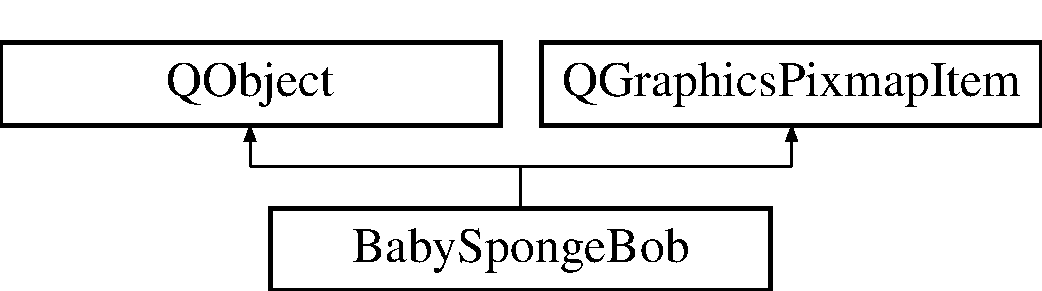
\includegraphics[height=2.000000cm]{classBabySpongeBob}
\end{center}
\end{figure}
\subsection*{Public Slots}
\begin{DoxyCompactItemize}
\item 
void \hyperlink{classBabySpongeBob_a64d2c583237fceaff5e99a23295f4119}{update} ()
\begin{DoxyCompactList}\small\item\em updates c \end{DoxyCompactList}\end{DoxyCompactItemize}
\subsection*{Public Member Functions}
\begin{DoxyCompactItemize}
\item 
\hyperlink{classBabySpongeBob_a1d0fe9d631ee9aee6b838ecf76bc00f2}{Baby\-Sponge\-Bob} (int \hyperlink{classBabySpongeBob_a072dca2ee666af5a39be11e152a04b2c}{healthy\-Items\-Fed}=0, Q\-Object $\ast$parent=nullptr)
\end{DoxyCompactItemize}
\subsection*{Public Attributes}
\begin{DoxyCompactItemize}
\item 
\hypertarget{classBabySpongeBob_acfb8d9ea28550ff76e80bf1adc335ad8}{Q\-Timer $\ast$ {\bfseries timer}}\label{classBabySpongeBob_acfb8d9ea28550ff76e80bf1adc335ad8}

\item 
\hypertarget{classBabySpongeBob_a072dca2ee666af5a39be11e152a04b2c}{int \hyperlink{classBabySpongeBob_a072dca2ee666af5a39be11e152a04b2c}{healthy\-Items\-Fed}}\label{classBabySpongeBob_a072dca2ee666af5a39be11e152a04b2c}

\begin{DoxyCompactList}\small\item\em this variable stores the number of healthy items fed to the baby \end{DoxyCompactList}\end{DoxyCompactItemize}


\subsection{Constructor \& Destructor Documentation}
\hypertarget{classBabySpongeBob_a1d0fe9d631ee9aee6b838ecf76bc00f2}{\index{Baby\-Sponge\-Bob@{Baby\-Sponge\-Bob}!Baby\-Sponge\-Bob@{Baby\-Sponge\-Bob}}
\index{Baby\-Sponge\-Bob@{Baby\-Sponge\-Bob}!BabySpongeBob@{Baby\-Sponge\-Bob}}
\subsubsection[{Baby\-Sponge\-Bob}]{\setlength{\rightskip}{0pt plus 5cm}Baby\-Sponge\-Bob\-::\-Baby\-Sponge\-Bob (
\begin{DoxyParamCaption}
\item[{int}]{healthy\-Items\-Fed = {\ttfamily 0}, }
\item[{Q\-Object $\ast$}]{parent = {\ttfamily nullptr}}
\end{DoxyParamCaption}
)\hspace{0.3cm}{\ttfamily [explicit]}}}\label{classBabySpongeBob_a1d0fe9d631ee9aee6b838ecf76bc00f2}
$<$ setting picture of baby

$<$ starting timer

$<$ setting number of healthy items already fed (in case of pause)

$<$ timer for update 

\subsection{Member Function Documentation}
\hypertarget{classBabySpongeBob_a64d2c583237fceaff5e99a23295f4119}{\index{Baby\-Sponge\-Bob@{Baby\-Sponge\-Bob}!update@{update}}
\index{update@{update}!BabySpongeBob@{Baby\-Sponge\-Bob}}
\subsubsection[{update}]{\setlength{\rightskip}{0pt plus 5cm}void Baby\-Sponge\-Bob\-::update (
\begin{DoxyParamCaption}
{}
\end{DoxyParamCaption}
)\hspace{0.3cm}{\ttfamily [slot]}}}\label{classBabySpongeBob_a64d2c583237fceaff5e99a23295f4119}


updates c 

\hyperlink{classBabySpongeBob_a64d2c583237fceaff5e99a23295f4119}{Baby\-Sponge\-Bob\-::update}, updates the game metrics in case an item reaches the baby. if the item is of type grabbable, the function reached\-Baby is called to update the metrics 

The documentation for this class was generated from the following files\-:\begin{DoxyCompactItemize}
\item 
babyspongebob.\-h\item 
\hyperlink{babyspongebob_8cpp}{babyspongebob.\-cpp}\end{DoxyCompactItemize}

\hypertarget{classbacteria}{\section{bacteria Class Reference}
\label{classbacteria}\index{bacteria@{bacteria}}
}


bacteria class  




{\ttfamily \#include $<$bacteria.\-h$>$}

Inheritance diagram for bacteria\-:\begin{figure}[H]
\begin{center}
\leavevmode
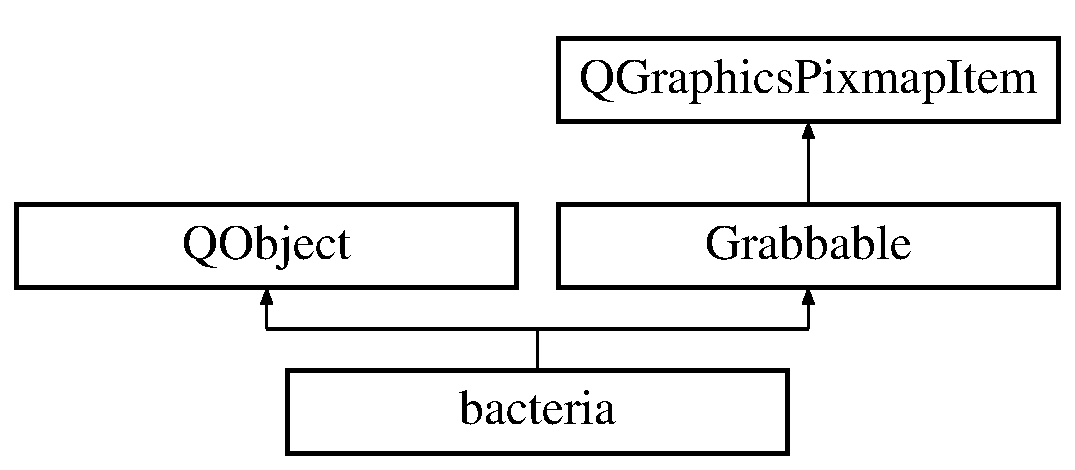
\includegraphics[height=3.000000cm]{classbacteria}
\end{center}
\end{figure}
\subsection*{Public Slots}
\begin{DoxyCompactItemize}
\item 
void \hyperlink{classbacteria_abbc6e655d055d64b1f506248b598f03a}{update} ()
\begin{DoxyCompactList}\small\item\em update the location on the screen and detects collisions \end{DoxyCompactList}\end{DoxyCompactItemize}
\subsection*{Public Member Functions}
\begin{DoxyCompactItemize}
\item 
\hyperlink{classbacteria_a9c1bb600d594429c64446a9dff56f398}{bacteria} (int strength, int \hyperlink{classbacteria_ae0262e42fe93ae2fcd6cb77f53be8d05}{direction}, int \hyperlink{classbacteria_ab4cdc40bc26aa012391f7543f7e0d54b}{direction\-Y}, double \hyperlink{classbacteria_a4b0a914494a4d5c26b12181f7546d3e1}{Xvelocity}, double \hyperlink{classbacteria_ab0faabfc046869969c36b88ecd105702}{Yvelocity}, int \hyperlink{classbacteria_aa97d75555e88a076c05dcc217b107b54}{deviation\-Limit}, int \hyperlink{classbacteria_a512cfc4c7afef0e3bf8f76bd53072de9}{centerline}, \hyperlink{classHeader}{Header} $\ast$\hyperlink{classGrabbable_a97db8193dec83a8086352f80a30b2038}{header}=N\-U\-L\-L, Q\-String game=\char`\"{}\char`\"{}, Q\-Object $\ast$parent=nullptr)
\item 
\hypertarget{classbacteria_afd6e4d4c7575387a8ffdcc7a40287507}{\hyperlink{classbacteria_afd6e4d4c7575387a8ffdcc7a40287507}{$\sim$bacteria} ()}\label{classbacteria_afd6e4d4c7575387a8ffdcc7a40287507}

\begin{DoxyCompactList}\small\item\em destructor \end{DoxyCompactList}\end{DoxyCompactItemize}
\subsection*{Public Attributes}
\begin{DoxyCompactItemize}
\item 
\hypertarget{classbacteria_a217dff93e774f9a55370636c5e0d1bef}{Q\-Timer $\ast$ \hyperlink{classbacteria_a217dff93e774f9a55370636c5e0d1bef}{timer}}\label{classbacteria_a217dff93e774f9a55370636c5e0d1bef}

\begin{DoxyCompactList}\small\item\em timer attribute that specifies the timer \end{DoxyCompactList}\item 
\hypertarget{classbacteria_ae0262e42fe93ae2fcd6cb77f53be8d05}{int \hyperlink{classbacteria_ae0262e42fe93ae2fcd6cb77f53be8d05}{direction}}\label{classbacteria_ae0262e42fe93ae2fcd6cb77f53be8d05}

\begin{DoxyCompactList}\small\item\em direction attribute that specifies the direction of movement of the bacteria \end{DoxyCompactList}\item 
\hypertarget{classbacteria_ab4cdc40bc26aa012391f7543f7e0d54b}{int \hyperlink{classbacteria_ab4cdc40bc26aa012391f7543f7e0d54b}{direction\-Y}}\label{classbacteria_ab4cdc40bc26aa012391f7543f7e0d54b}

\begin{DoxyCompactList}\small\item\em attribute that specifies the Y direction of movement of the virus \end{DoxyCompactList}\item 
\hypertarget{classbacteria_a4b0a914494a4d5c26b12181f7546d3e1}{int \hyperlink{classbacteria_a4b0a914494a4d5c26b12181f7546d3e1}{Xvelocity}}\label{classbacteria_a4b0a914494a4d5c26b12181f7546d3e1}

\begin{DoxyCompactList}\small\item\em attribute that specifies the X velocity of the virus \end{DoxyCompactList}\item 
\hypertarget{classbacteria_ab0faabfc046869969c36b88ecd105702}{int \hyperlink{classbacteria_ab0faabfc046869969c36b88ecd105702}{Yvelocity}}\label{classbacteria_ab0faabfc046869969c36b88ecd105702}

\begin{DoxyCompactList}\small\item\em attribute that specifies the X velocity of the virus \end{DoxyCompactList}\item 
\hypertarget{classbacteria_aa97d75555e88a076c05dcc217b107b54}{int \hyperlink{classbacteria_aa97d75555e88a076c05dcc217b107b54}{deviation\-Limit}}\label{classbacteria_aa97d75555e88a076c05dcc217b107b54}

\begin{DoxyCompactList}\small\item\em specifies maximum deviation from center line \end{DoxyCompactList}\item 
\hypertarget{classbacteria_a512cfc4c7afef0e3bf8f76bd53072de9}{int \hyperlink{classbacteria_a512cfc4c7afef0e3bf8f76bd53072de9}{centerline}}\label{classbacteria_a512cfc4c7afef0e3bf8f76bd53072de9}

\begin{DoxyCompactList}\small\item\em specifies the center of propagation of the virus \end{DoxyCompactList}\item 
\hypertarget{classbacteria_ab7647c95c379933e91925ef1222cf05b}{int {\bfseries upperlimit}}\label{classbacteria_ab7647c95c379933e91925ef1222cf05b}

\item 
\hypertarget{classbacteria_a16f904a662cd13a7dfaf230f8e4a1436}{Q\-String {\bfseries game}}\label{classbacteria_a16f904a662cd13a7dfaf230f8e4a1436}

\end{DoxyCompactItemize}


\subsection{Detailed Description}
bacteria class 

.h A bacteria is an element on screen that moves periodically in a predefined direction. 

\subsection{Constructor \& Destructor Documentation}
\hypertarget{classbacteria_a9c1bb600d594429c64446a9dff56f398}{\index{bacteria@{bacteria}!bacteria@{bacteria}}
\index{bacteria@{bacteria}!bacteria@{bacteria}}
\subsubsection[{bacteria}]{\setlength{\rightskip}{0pt plus 5cm}bacteria\-::bacteria (
\begin{DoxyParamCaption}
\item[{int}]{strength, }
\item[{int}]{direction, }
\item[{int}]{direction\-Y, }
\item[{double}]{Xvelocity, }
\item[{double}]{Yvelocity, }
\item[{int}]{deviation\-Limit, }
\item[{int}]{centerline, }
\item[{{\bf Header} $\ast$}]{header = {\ttfamily NULL}, }
\item[{Q\-String}]{game = {\ttfamily \char`\"{}\char`\"{}}, }
\item[{Q\-Object $\ast$}]{parent = {\ttfamily nullptr}}
\end{DoxyParamCaption}
)\hspace{0.3cm}{\ttfamily [explicit]}}}\label{classbacteria_a9c1bb600d594429c64446a9dff56f398}
setting attributes

starting timer and connecting it 

\subsection{Member Function Documentation}
\hypertarget{classbacteria_abbc6e655d055d64b1f506248b598f03a}{\index{bacteria@{bacteria}!update@{update}}
\index{update@{update}!bacteria@{bacteria}}
\subsubsection[{update}]{\setlength{\rightskip}{0pt plus 5cm}void bacteria\-::update (
\begin{DoxyParamCaption}
{}
\end{DoxyParamCaption}
)\hspace{0.3cm}{\ttfamily [slot]}}}\label{classbacteria_abbc6e655d055d64b1f506248b598f03a}


update the location on the screen and detects collisions 

\hyperlink{classbacteria_abbc6e655d055d64b1f506248b598f03a}{bacteria\-::update} updated the position of the bacteria. It also checks if theres is a collision with any object and checks its type. additionally, it updates the metrics if there is a collision with the player (spongebob) checks if the item is at the boundary of the screen to remove it

checks if there is a collision

checks if the collision is with the player

$<$checking if the player isnt strong enough to kill the bacteria, if true, he should lose a life.

update lives, deletes item,updates cleanliness, and reset stats

$<$ player is strong enough to kill the bacteria

deletes item,updates cleanliness, and updates stats

updating item position if the player has the followme tag toggled on, this means that the bacteria should follow him. an algorithm is used to calculate the speed and direction at which the item should move to follow the palyer.

else, the bacteria moves in a wave motion along a fixed center line form the left to the right or the opposite based on its direction.

algorithm to follow the plater 

The documentation for this class was generated from the following files\-:\begin{DoxyCompactItemize}
\item 
bacteria.\-h\item 
\hyperlink{bacteria_8cpp}{bacteria.\-cpp}\end{DoxyCompactItemize}

\hypertarget{classBomb}{\section{Bomb Class Reference}
\label{classBomb}\index{Bomb@{Bomb}}
}
Inheritance diagram for Bomb\-:\begin{figure}[H]
\begin{center}
\leavevmode
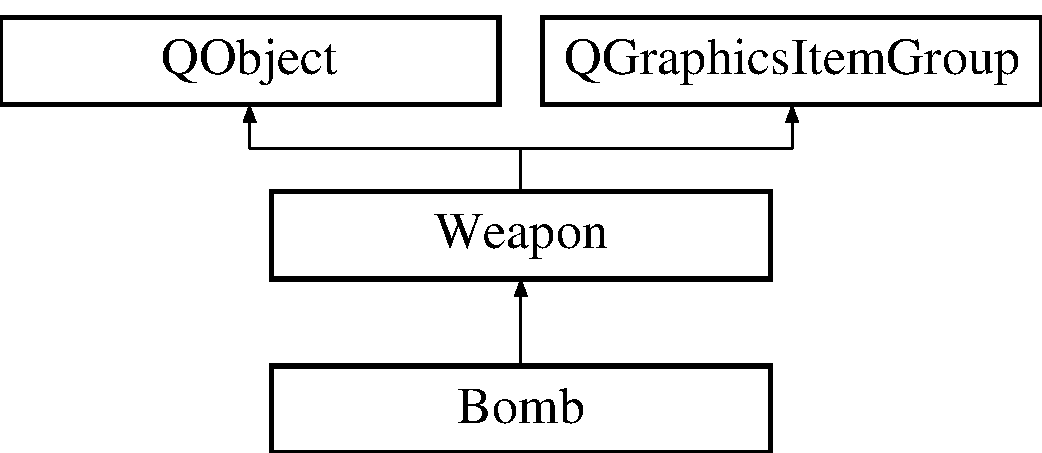
\includegraphics[height=3.000000cm]{classBomb}
\end{center}
\end{figure}
\subsection*{Public Slots}
\begin{DoxyCompactItemize}
\item 
void \hyperlink{classBomb_a6fa3577a6653276f456aff457062fbc1}{update} ()
\begin{DoxyCompactList}\small\item\em \hyperlink{classBomb_a6fa3577a6653276f456aff457062fbc1}{Bomb\-::update} updates the position of the bomb and checks for collision. \end{DoxyCompactList}\end{DoxyCompactItemize}
\subsection*{Public Member Functions}
\begin{DoxyCompactItemize}
\item 
\hyperlink{classBomb_ab2a76ef6357e7840ed410df60cc980e5}{Bomb} (int strength)
\begin{DoxyCompactList}\small\item\em \hyperlink{classBomb_ab2a76ef6357e7840ed410df60cc980e5}{Bomb\-::\-Bomb} constructor. \end{DoxyCompactList}\end{DoxyCompactItemize}
\subsection*{Additional Inherited Members}


\subsection{Constructor \& Destructor Documentation}
\hypertarget{classBomb_ab2a76ef6357e7840ed410df60cc980e5}{\index{Bomb@{Bomb}!Bomb@{Bomb}}
\index{Bomb@{Bomb}!Bomb@{Bomb}}
\subsubsection[{Bomb}]{\setlength{\rightskip}{0pt plus 5cm}Bomb\-::\-Bomb (
\begin{DoxyParamCaption}
\item[{int}]{strength}
\end{DoxyParamCaption}
)}}\label{classBomb_ab2a76ef6357e7840ed410df60cc980e5}


\hyperlink{classBomb_ab2a76ef6357e7840ed410df60cc980e5}{Bomb\-::\-Bomb} constructor. 


\begin{DoxyParams}{Parameters}
{\em strength} & the strength of the bomb ( how fast it goes) \\
\hline
\end{DoxyParams}
setting attributes 

\subsection{Member Function Documentation}
\hypertarget{classBomb_a6fa3577a6653276f456aff457062fbc1}{\index{Bomb@{Bomb}!update@{update}}
\index{update@{update}!Bomb@{Bomb}}
\subsubsection[{update}]{\setlength{\rightskip}{0pt plus 5cm}void Bomb\-::update (
\begin{DoxyParamCaption}
{}
\end{DoxyParamCaption}
)\hspace{0.3cm}{\ttfamily [slot]}}}\label{classBomb_a6fa3577a6653276f456aff457062fbc1}


\hyperlink{classBomb_a6fa3577a6653276f456aff457062fbc1}{Bomb\-::update} updates the position of the bomb and checks for collision. 

if not ready to throw the bomb, setting it.

$<$ adding number of steps passed.

there is a collision with an item that is grabbable,there are items to delete.

number of teps exceeds limit. bomb is deleted 

The documentation for this class was generated from the following files\-:\begin{DoxyCompactItemize}
\item 
bomb.\-h\item 
\hyperlink{bomb_8cpp}{bomb.\-cpp}\end{DoxyCompactItemize}

\hypertarget{classcheat}{\section{cheat Class Reference}
\label{classcheat}\index{cheat@{cheat}}
}
Inheritance diagram for cheat\-:\begin{figure}[H]
\begin{center}
\leavevmode
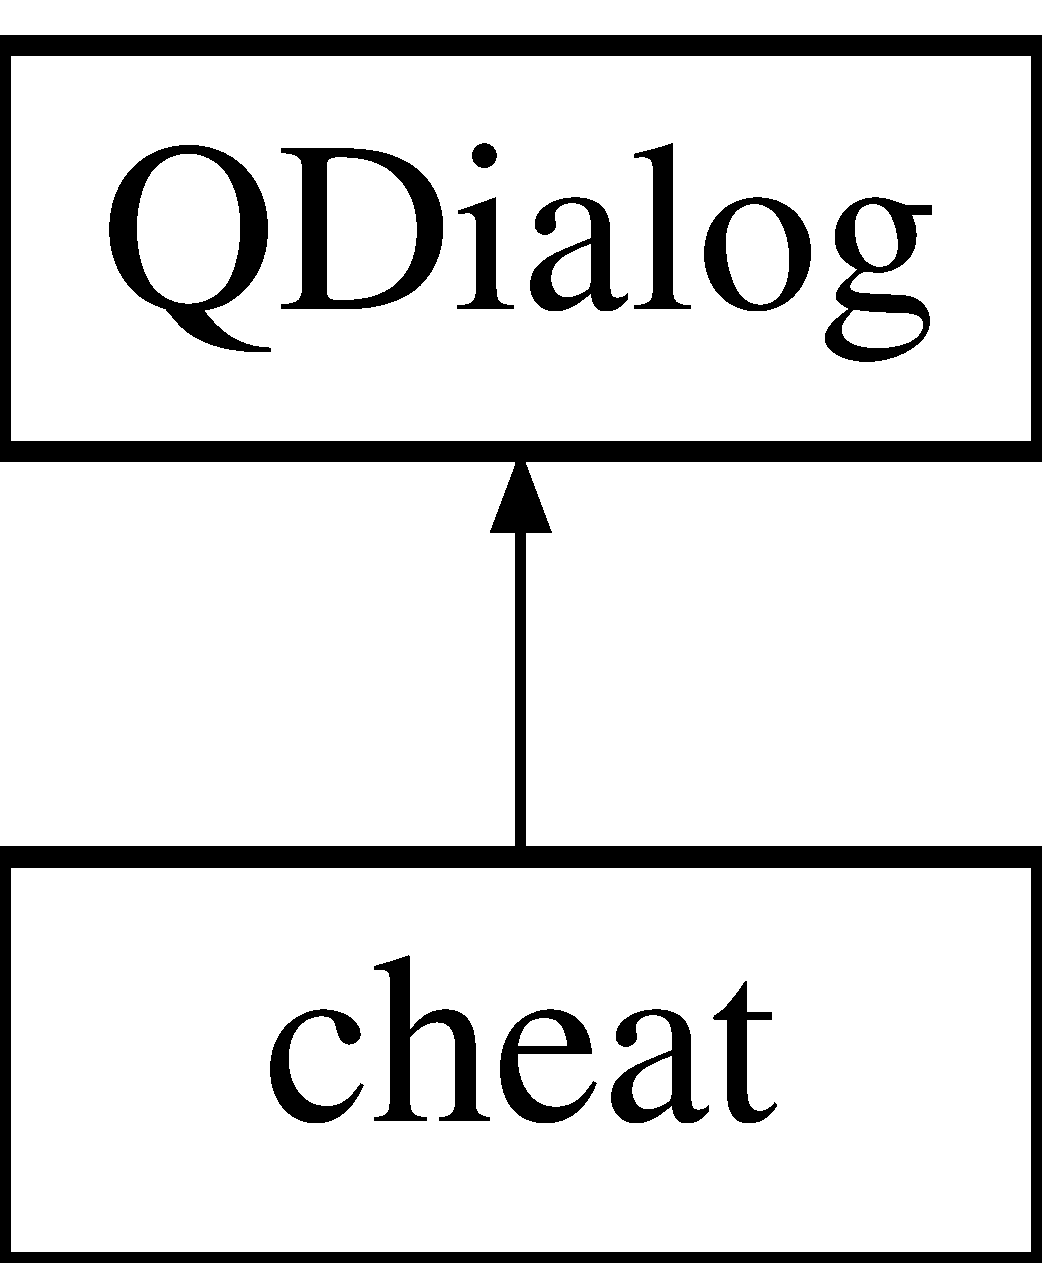
\includegraphics[height=2.000000cm]{classcheat}
\end{center}
\end{figure}
\subsection*{Public Member Functions}
\begin{DoxyCompactItemize}
\item 
\hypertarget{classcheat_af46a9a0276d8ace2bc3f4e835fb153b5}{{\bfseries cheat} (Q\-Widget $\ast$parent=0)}\label{classcheat_af46a9a0276d8ace2bc3f4e835fb153b5}

\end{DoxyCompactItemize}


The documentation for this class was generated from the following files\-:\begin{DoxyCompactItemize}
\item 
cheat.\-h\item 
\hyperlink{cheat_8cpp}{cheat.\-cpp}\end{DoxyCompactItemize}

\hypertarget{classCleanlinessMeter}{\section{Cleanliness\-Meter Class Reference}
\label{classCleanlinessMeter}\index{Cleanliness\-Meter@{Cleanliness\-Meter}}
}
Inheritance diagram for Cleanliness\-Meter\-:\begin{figure}[H]
\begin{center}
\leavevmode
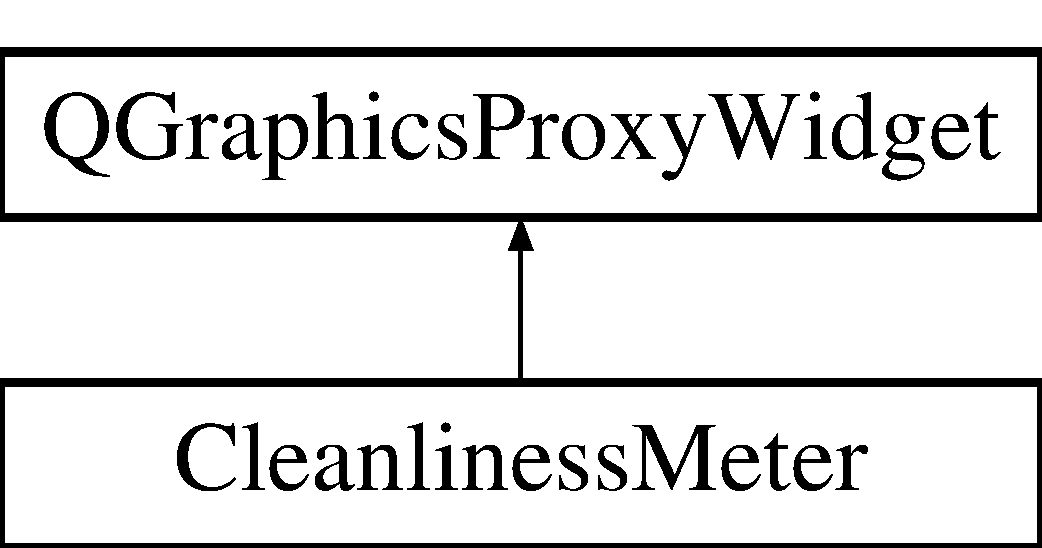
\includegraphics[height=2.000000cm]{classCleanlinessMeter}
\end{center}
\end{figure}
\subsection*{Public Member Functions}
\begin{DoxyCompactItemize}
\item 
\hypertarget{classCleanlinessMeter_aa6c6dbca9a896e45b2b79ce4065f5276}{void {\bfseries Update\-Value} ()}\label{classCleanlinessMeter_aa6c6dbca9a896e45b2b79ce4065f5276}

\end{DoxyCompactItemize}
\subsection*{Public Attributes}
\begin{DoxyCompactItemize}
\item 
\hypertarget{classCleanlinessMeter_a4e0c38787ca511a4041547a32504d93a}{Q\-Progress\-Bar $\ast$ {\bfseries Progress\-Bar}}\label{classCleanlinessMeter_a4e0c38787ca511a4041547a32504d93a}

\end{DoxyCompactItemize}


The documentation for this class was generated from the following files\-:\begin{DoxyCompactItemize}
\item 
cleanlinessmeter.\-h\item 
cleanlinessmeter.\-cpp\end{DoxyCompactItemize}

\hypertarget{classDescription}{\section{Description Class Reference}
\label{classDescription}\index{Description@{Description}}
}
Inheritance diagram for Description\-:\begin{figure}[H]
\begin{center}
\leavevmode
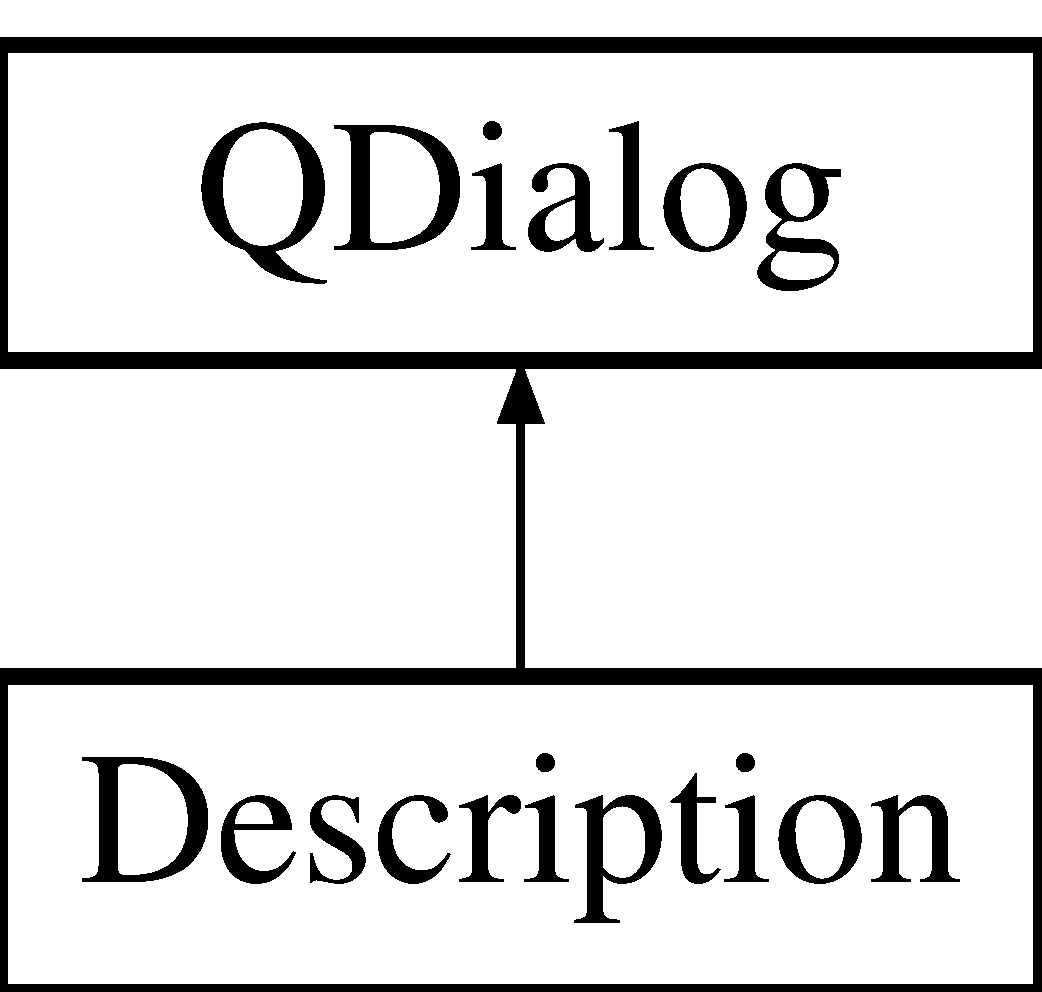
\includegraphics[height=2.000000cm]{classDescription}
\end{center}
\end{figure}
\subsection*{Public Member Functions}
\begin{DoxyCompactItemize}
\item 
\hypertarget{classDescription_aff75945f12c14cffd410cf456ddbfb27}{{\bfseries Description} (Q\-Widget $\ast$parent=0, Q\-String game=\char`\"{}\char`\"{})}\label{classDescription_aff75945f12c14cffd410cf456ddbfb27}

\end{DoxyCompactItemize}
\subsection*{Public Attributes}
\begin{DoxyCompactItemize}
\item 
\hypertarget{classDescription_a540e784e9116b5060c4573d37f4e6157}{Q\-String {\bfseries Game}}\label{classDescription_a540e784e9116b5060c4573d37f4e6157}

\end{DoxyCompactItemize}


The documentation for this class was generated from the following files\-:\begin{DoxyCompactItemize}
\item 
description.\-h\item 
\hyperlink{description_8cpp}{description.\-cpp}\end{DoxyCompactItemize}

\hypertarget{classError}{\section{Error Class Reference}
\label{classError}\index{Error@{Error}}
}
Inheritance diagram for Error\-:\begin{figure}[H]
\begin{center}
\leavevmode
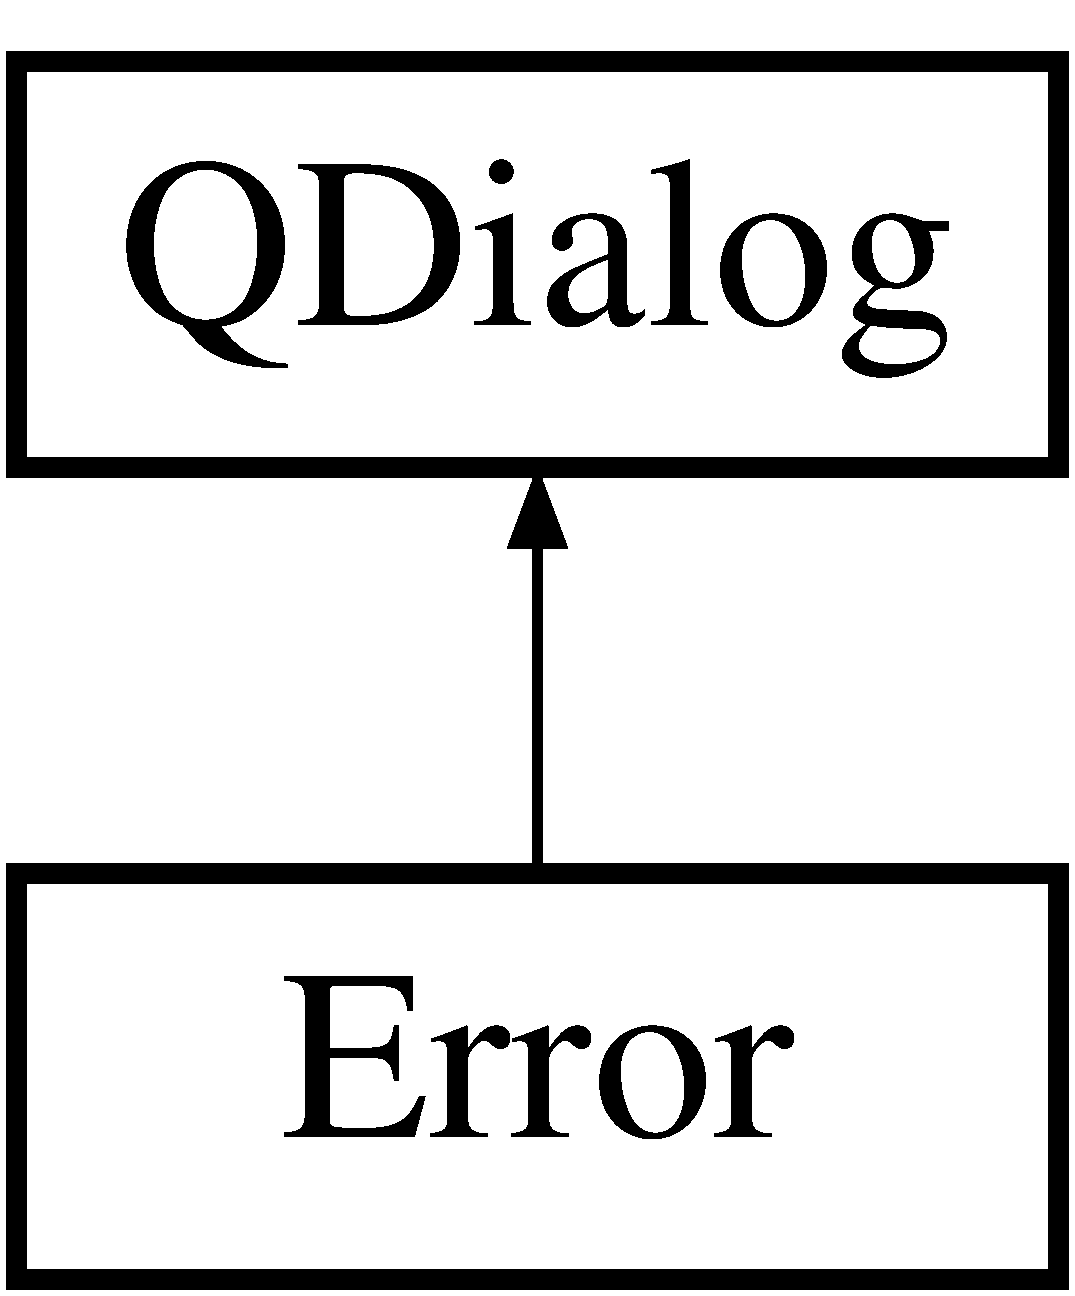
\includegraphics[height=2.000000cm]{classError}
\end{center}
\end{figure}
\subsection*{Public Member Functions}
\begin{DoxyCompactItemize}
\item 
\hypertarget{classError_a024638e93b49ba6024aa01eadb0f9d5b}{{\bfseries Error} (Q\-String msg, Q\-Widget $\ast$parent=0)}\label{classError_a024638e93b49ba6024aa01eadb0f9d5b}

\end{DoxyCompactItemize}


The documentation for this class was generated from the following files\-:\begin{DoxyCompactItemize}
\item 
error.\-h\item 
\hyperlink{error_8cpp}{error.\-cpp}\end{DoxyCompactItemize}

\hypertarget{classfungus}{\section{fungus Class Reference}
\label{classfungus}\index{fungus@{fungus}}
}


fungus class  




{\ttfamily \#include $<$fungus.\-h$>$}

Inheritance diagram for fungus\-:\begin{figure}[H]
\begin{center}
\leavevmode
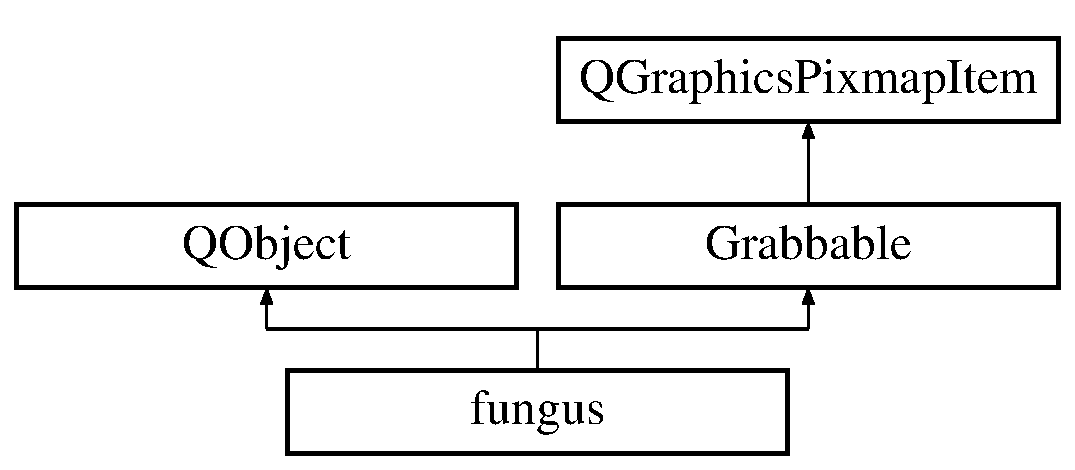
\includegraphics[height=3.000000cm]{classfungus}
\end{center}
\end{figure}
\subsection*{Public Slots}
\begin{DoxyCompactItemize}
\item 
void \hyperlink{classfungus_a2eb2952502ef6a467163a764f0cb773d}{update} ()
\begin{DoxyCompactList}\small\item\em update the location on the screen and detects collisions \end{DoxyCompactList}\end{DoxyCompactItemize}
\subsection*{Public Member Functions}
\begin{DoxyCompactItemize}
\item 
\hyperlink{classfungus_a5387ba07067ee3306649b4aa900b2c5d}{fungus} (\hyperlink{classHeader}{Header} $\ast$\hyperlink{classGrabbable_a97db8193dec83a8086352f80a30b2038}{header}, Q\-String name=\char`\"{}\char`\"{}, Q\-Object $\ast$parent=nullptr)
\begin{DoxyCompactList}\small\item\em \hyperlink{classfungus_a5387ba07067ee3306649b4aa900b2c5d}{fungus\-::fungus} \end{DoxyCompactList}\end{DoxyCompactItemize}
\subsection*{Public Attributes}
\begin{DoxyCompactItemize}
\item 
\hypertarget{classfungus_ab537a12540fff0570026e58b48eec29d}{Q\-Timer $\ast$ \hyperlink{classfungus_ab537a12540fff0570026e58b48eec29d}{timer}}\label{classfungus_ab537a12540fff0570026e58b48eec29d}

\begin{DoxyCompactList}\small\item\em timer attribute that specifies the timer \end{DoxyCompactList}\item 
\hypertarget{classfungus_a41c3791a53d9f8f137c5c519d0cd0742}{int \hyperlink{classfungus_a41c3791a53d9f8f137c5c519d0cd0742}{Xvelocity}}\label{classfungus_a41c3791a53d9f8f137c5c519d0cd0742}

\begin{DoxyCompactList}\small\item\em y velocity of fungus \end{DoxyCompactList}\item 
\hypertarget{classfungus_acf88a26542582ba595fce0d65d2c8f16}{int \hyperlink{classfungus_acf88a26542582ba595fce0d65d2c8f16}{Yvelocity}}\label{classfungus_acf88a26542582ba595fce0d65d2c8f16}

\begin{DoxyCompactList}\small\item\em x velocity of fungus \end{DoxyCompactList}\item 
\hypertarget{classfungus_a3a90ae49c71638d579aadd54c9a8424e}{int \hyperlink{classfungus_a3a90ae49c71638d579aadd54c9a8424e}{timetolive}}\label{classfungus_a3a90ae49c71638d579aadd54c9a8424e}

\begin{DoxyCompactList}\small\item\em specifies time left to die \end{DoxyCompactList}\item 
\hypertarget{classfungus_af5778c05c2d02dad47586b22b35cd4fd}{Q\-String {\bfseries game}}\label{classfungus_af5778c05c2d02dad47586b22b35cd4fd}

\end{DoxyCompactItemize}


\subsection{Detailed Description}
fungus class 

.h A fungus is an element on screen that moves periodically following spongebob. 

\subsection{Constructor \& Destructor Documentation}
\hypertarget{classfungus_a5387ba07067ee3306649b4aa900b2c5d}{\index{fungus@{fungus}!fungus@{fungus}}
\index{fungus@{fungus}!fungus@{fungus}}
\subsubsection[{fungus}]{\setlength{\rightskip}{0pt plus 5cm}fungus\-::fungus (
\begin{DoxyParamCaption}
\item[{{\bf Header} $\ast$}]{header, }
\item[{Q\-String}]{game = {\ttfamily \char`\"{}\char`\"{}}, }
\item[{Q\-Object $\ast$}]{parent = {\ttfamily nullptr}}
\end{DoxyParamCaption}
)\hspace{0.3cm}{\ttfamily [explicit]}}}\label{classfungus_a5387ba07067ee3306649b4aa900b2c5d}


\hyperlink{classfungus_a5387ba07067ee3306649b4aa900b2c5d}{fungus\-::fungus} 


\begin{DoxyParams}{Parameters}
{\em header} & \\
\hline
{\em parent} & constructor of a fungus, creates an instance and provides is with a velocity, time to live, and a pointer to the header \\
\hline
\end{DoxyParams}


\subsection{Member Function Documentation}
\hypertarget{classfungus_a2eb2952502ef6a467163a764f0cb773d}{\index{fungus@{fungus}!update@{update}}
\index{update@{update}!fungus@{fungus}}
\subsubsection[{update}]{\setlength{\rightskip}{0pt plus 5cm}void fungus\-::update (
\begin{DoxyParamCaption}
{}
\end{DoxyParamCaption}
)\hspace{0.3cm}{\ttfamily [slot]}}}\label{classfungus_a2eb2952502ef6a467163a764f0cb773d}


update the location on the screen and detects collisions 

\hyperlink{classfungus_a2eb2952502ef6a467163a764f0cb773d}{fungus\-::update}

updates the position, detects collision, and in case of collision with the player, it penalises him it also deletes the fungus if its time is over collidelist this creates a list of all colliding items. it then dynamically casts each detected item to an instance of spongebob if any item returns true which means that it exists, this means that a collision with spongebob has occured this leads to some procedures

immunity is halved

cleanliness is halved

instructs batceria to follow him

timer for following starts

this is an algorithm to detect the position of spongebob and follow him 

The documentation for this class was generated from the following files\-:\begin{DoxyCompactItemize}
\item 
fungus.\-h\item 
\hyperlink{fungus_8cpp}{fungus.\-cpp}\end{DoxyCompactItemize}

\hypertarget{classGame}{\section{Game Class Reference}
\label{classGame}\index{Game@{Game}}
}
Inheritance diagram for Game\-:\begin{figure}[H]
\begin{center}
\leavevmode
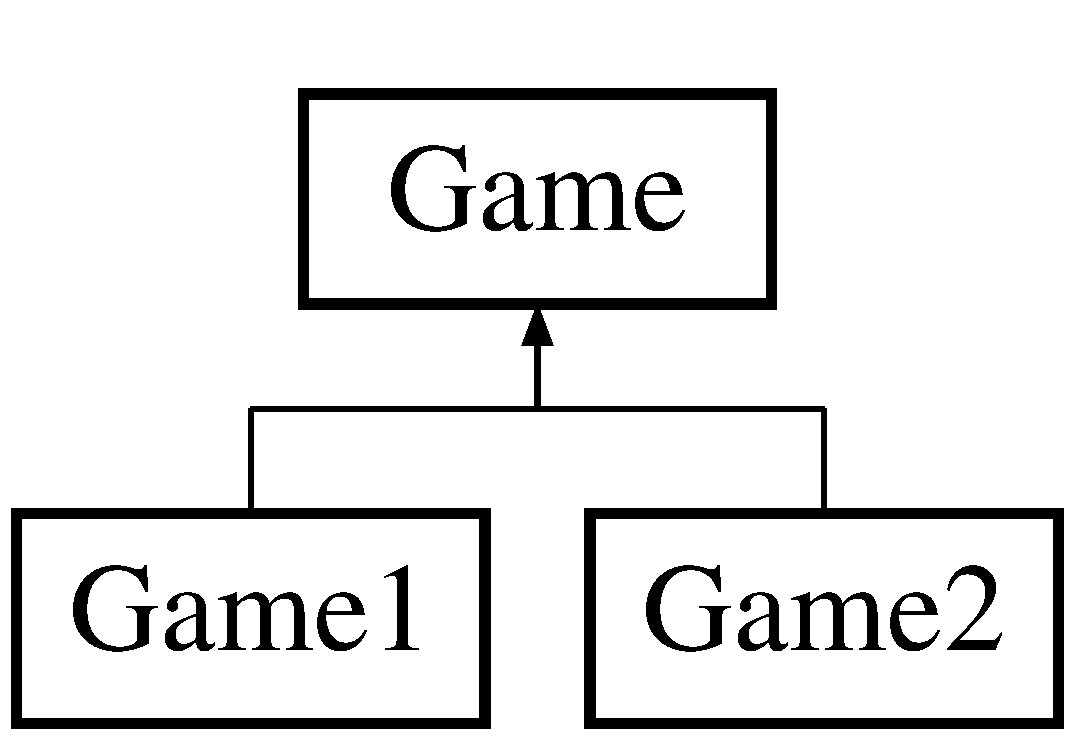
\includegraphics[height=2.000000cm]{classGame}
\end{center}
\end{figure}
\subsection*{Public Types}
\begin{DoxyCompactItemize}
\item 
enum {\bfseries Game\-Difficulty} \{ {\bfseries easy} = 1, 
{\bfseries medium} = 2, 
{\bfseries hard} = 3
 \}
\item 
enum {\bfseries Game\-Mode} \{ \\*
{\bfseries New} = 1, 
{\bfseries Resume} = 2, 
{\bfseries Over} = 3, 
{\bfseries Win} = 4, 
\\*
{\bfseries Pause} = 5
 \}
\end{DoxyCompactItemize}
\subsection*{Public Member Functions}
\begin{DoxyCompactItemize}
\item 
\hypertarget{classGame_a540a40b348041ce60ba1214cb61e5118}{void {\bfseries Set\-Difficulty} (bool easy\-Radio, bool medium\-Radio, bool hard\-Radio)}\label{classGame_a540a40b348041ce60ba1214cb61e5118}

\end{DoxyCompactItemize}
\subsection*{Public Attributes}
\begin{DoxyCompactItemize}
\item 
\hypertarget{classGame_af5aeb877034a1c72a571750907358b41}{\hyperlink{classUser}{User} $\ast$ {\bfseries user}}\label{classGame_af5aeb877034a1c72a571750907358b41}

\item 
\hypertarget{classGame_ad02dbd2a814db8589c53b059d4201fe7}{int {\bfseries Difficulty}}\label{classGame_ad02dbd2a814db8589c53b059d4201fe7}

\item 
\hypertarget{classGame_a06ea7da9354fa9d08731a3db219d2566}{\hyperlink{classGameView}{Game\-View} $\ast$ {\bfseries game\-View}}\label{classGame_a06ea7da9354fa9d08731a3db219d2566}

\end{DoxyCompactItemize}


The documentation for this class was generated from the following files\-:\begin{DoxyCompactItemize}
\item 
game.\-h\item 
game.\-cpp\end{DoxyCompactItemize}

\hypertarget{classGame1}{\section{Game1 Class Reference}
\label{classGame1}\index{Game1@{Game1}}
}
Inheritance diagram for Game1\-:\begin{figure}[H]
\begin{center}
\leavevmode
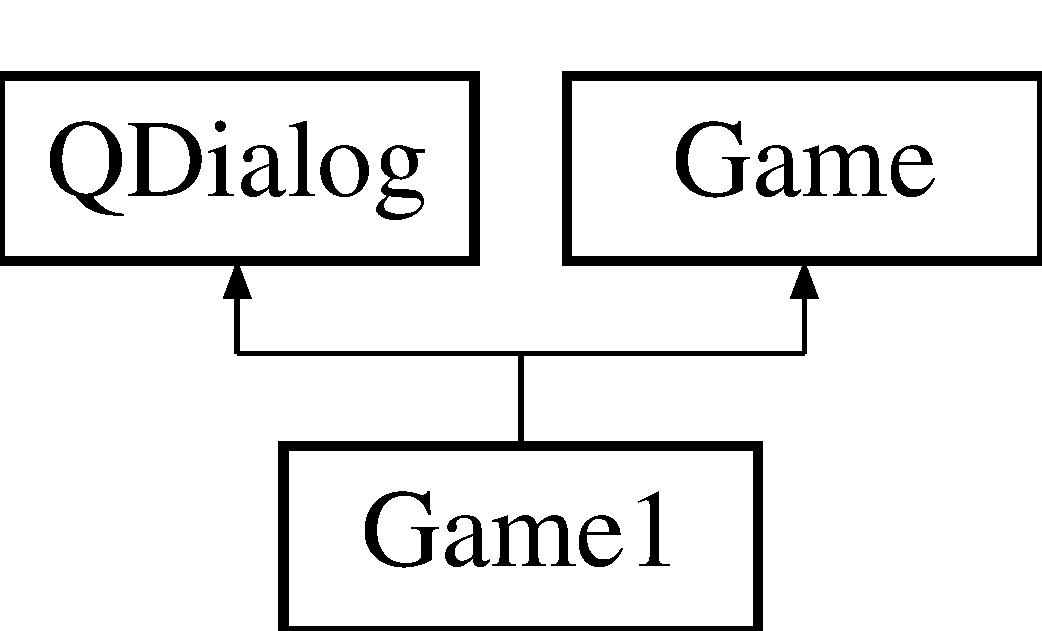
\includegraphics[height=2.000000cm]{classGame1}
\end{center}
\end{figure}
\subsection*{Public Member Functions}
\begin{DoxyCompactItemize}
\item 
\hyperlink{classGame1_a151ee9fa2f4899fa571971b8d1fcd551}{Game1} (Q\-Widget $\ast$parent=0, \hyperlink{classUser}{User} $\ast$user=new \hyperlink{classUser}{User}())
\begin{DoxyCompactList}\small\item\em \hyperlink{classGame1_a151ee9fa2f4899fa571971b8d1fcd551}{Game1\-::\-Game1} constructor for the class. it also sets the radio buttons to enabled or disabled based on the players previous records. \end{DoxyCompactList}\item 
\hypertarget{classGame1_aa498b4499c4032cc7a65cc7755b1d3be}{\hyperlink{classGame1_aa498b4499c4032cc7a65cc7755b1d3be}{$\sim$\-Game1} ()}\label{classGame1_aa498b4499c4032cc7a65cc7755b1d3be}

\begin{DoxyCompactList}\small\item\em distructor \end{DoxyCompactList}\end{DoxyCompactItemize}
\subsection*{Static Public Attributes}
\begin{DoxyCompactItemize}
\item 
\hypertarget{classGame1_ad07b4333580894f280ac4c45e46bb83c}{static Q\-String {\bfseries name} = \char`\"{}Game1\char`\"{}}\label{classGame1_ad07b4333580894f280ac4c45e46bb83c}

\end{DoxyCompactItemize}
\subsection*{Additional Inherited Members}


\subsection{Constructor \& Destructor Documentation}
\hypertarget{classGame1_a151ee9fa2f4899fa571971b8d1fcd551}{\index{Game1@{Game1}!Game1@{Game1}}
\index{Game1@{Game1}!Game1@{Game1}}
\subsubsection[{Game1}]{\setlength{\rightskip}{0pt plus 5cm}Game1\-::\-Game1 (
\begin{DoxyParamCaption}
\item[{Q\-Widget $\ast$}]{parent = {\ttfamily 0}, }
\item[{{\bf User} $\ast$}]{user = {\ttfamily new~{\bf User}()}}
\end{DoxyParamCaption}
)\hspace{0.3cm}{\ttfamily [explicit]}}}\label{classGame1_a151ee9fa2f4899fa571971b8d1fcd551}


\hyperlink{classGame1_a151ee9fa2f4899fa571971b8d1fcd551}{Game1\-::\-Game1} constructor for the class. it also sets the radio buttons to enabled or disabled based on the players previous records. 


\begin{DoxyParams}{Parameters}
{\em parent} & \\
\hline
{\em user} & \\
\hline
\end{DoxyParams}
getting previous records 

The documentation for this class was generated from the following files\-:\begin{DoxyCompactItemize}
\item 
game1.\-h\item 
\hyperlink{game1_8cpp}{game1.\-cpp}\end{DoxyCompactItemize}

\hypertarget{classgame1scene}{\section{game1scene Class Reference}
\label{classgame1scene}\index{game1scene@{game1scene}}
}


\hyperlink{classgame1scene}{game1scene} class  




{\ttfamily \#include $<$game1scene.\-h$>$}

Inheritance diagram for game1scene\-:\begin{figure}[H]
\begin{center}
\leavevmode
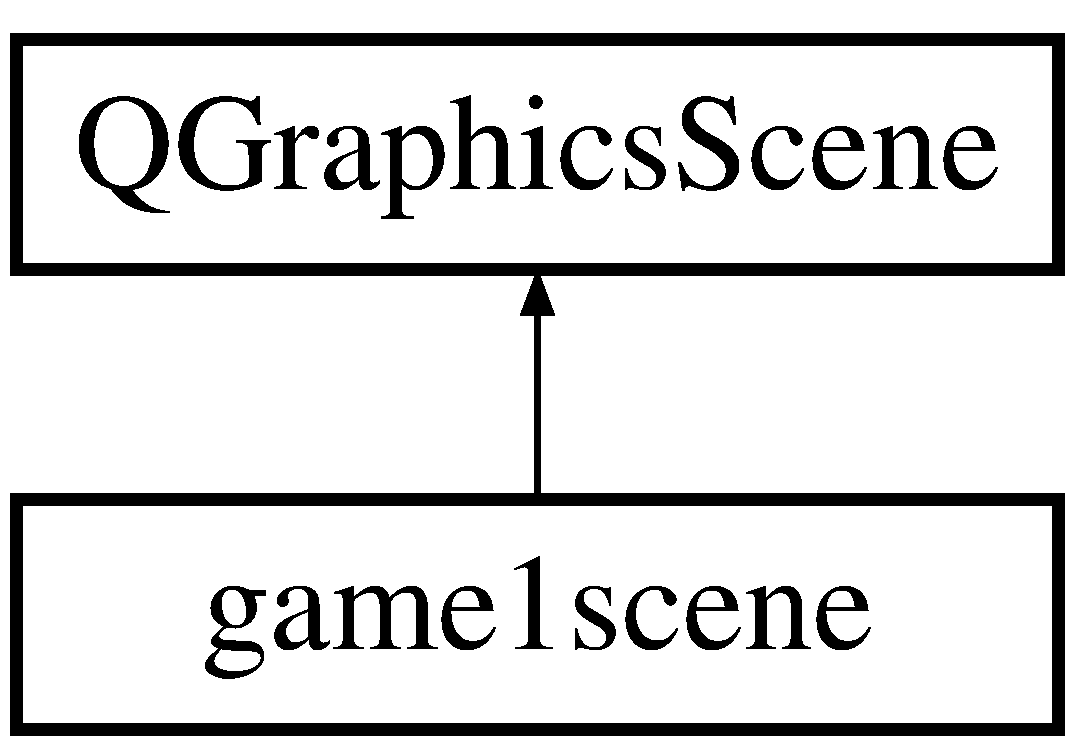
\includegraphics[height=2.000000cm]{classgame1scene}
\end{center}
\end{figure}
\subsection*{Public Slots}
\begin{DoxyCompactItemize}
\item 
void \hyperlink{classgame1scene_a8df6dd08b6c8af1846612a967ad44f4a}{addhu\-Items} ()
\begin{DoxyCompactList}\small\item\em add hu\-Items on the screen \end{DoxyCompactList}\item 
void \hyperlink{classgame1scene_ae3d9c421c6c328769c83933533017f2d}{addbacteria} ()
\begin{DoxyCompactList}\small\item\em add bacteria on the screen \end{DoxyCompactList}\item 
void \hyperlink{classgame1scene_a2488f3cbaa02776cbb0963af8c07b97f}{addvirus} ()
\begin{DoxyCompactList}\small\item\em add viruses on the screen \end{DoxyCompactList}\item 
void \hyperlink{classgame1scene_aa4a059bf4feb9b5858b6f486dbbb1ff7}{addfungus} ()
\begin{DoxyCompactList}\small\item\em add fungii on the screen \end{DoxyCompactList}\item 
void \hyperlink{classgame1scene_add7e3b72a6fe43d4ace0059ef2c29efc}{Close\-View} ()
\begin{DoxyCompactList}\small\item\em \hyperlink{classgame1scene_add7e3b72a6fe43d4ace0059ef2c29efc}{game1scene\-::\-Close\-View} \end{DoxyCompactList}\end{DoxyCompactItemize}
\subsection*{Public Member Functions}
\begin{DoxyCompactItemize}
\item 
\hyperlink{classgame1scene_a6f8ab141252ed97f4ebcf242490a5fb5}{game1scene} (\hyperlink{classGameView}{Game\-View} $\ast$game\-View, int game\-Mode, Q\-String username, int difficulty=1, \hyperlink{classHeader}{Header} $\ast$\hyperlink{classgame1scene_a706c8a5b1b10c15dcbff1f0c57cba83a}{header}=nullptr, bool paused=false)
\begin{DoxyCompactList}\small\item\em constructor \end{DoxyCompactList}\item 
void \hyperlink{classgame1scene_a1751ec31c026f539c88b5c4540d6299c}{Game\-Over} ()
\begin{DoxyCompactList}\small\item\em \hyperlink{classgame1scene_a1751ec31c026f539c88b5c4540d6299c}{game1scene\-::\-Game\-Over} \end{DoxyCompactList}\item 
void \hyperlink{classgame1scene_a222ff5efee99acaca254846cf6faef73}{Won\-Game} ()
\begin{DoxyCompactList}\small\item\em \hyperlink{classgame1scene_a222ff5efee99acaca254846cf6faef73}{game1scene\-::\-Won\-Game} \end{DoxyCompactList}\item 
void \hyperlink{classgame1scene_a45b308a5aafab7382a414365f32b9014}{Pause\-Game} ()
\begin{DoxyCompactList}\small\item\em \hyperlink{classgame1scene_a45b308a5aafab7382a414365f32b9014}{game1scene\-::\-Pause\-Game} \end{DoxyCompactList}\item 
\hypertarget{classgame1scene_a90dccedd11f6f50c346e957a3408c40f}{void {\bfseries key\-Press\-Event} (Q\-Key\-Event $\ast$event)}\label{classgame1scene_a90dccedd11f6f50c346e957a3408c40f}

\item 
void \hyperlink{classgame1scene_a71aae166af3fd9976b870653535a1fd3}{key\-Release\-Event} (Q\-Key\-Event $\ast$event)
\begin{DoxyCompactList}\small\item\em Detects key release events. \end{DoxyCompactList}\item 
\hypertarget{classgame1scene_a8a850d31dab5b9a7bb3249622c89fca9}{void {\bfseries mouse\-Release\-Event} (Q\-Graphics\-Scene\-Mouse\-Event $\ast$event)}\label{classgame1scene_a8a850d31dab5b9a7bb3249622c89fca9}

\end{DoxyCompactItemize}
\subsection*{Public Attributes}
\begin{DoxyCompactItemize}
\item 
\hypertarget{classgame1scene_a706c8a5b1b10c15dcbff1f0c57cba83a}{\hyperlink{classHeader}{Header} $\ast$ \hyperlink{classgame1scene_a706c8a5b1b10c15dcbff1f0c57cba83a}{header}}\label{classgame1scene_a706c8a5b1b10c15dcbff1f0c57cba83a}

\begin{DoxyCompactList}\small\item\em pointer to header \end{DoxyCompactList}\item 
\hypertarget{classgame1scene_ad2c72f6792e05651ba8f8487e3359bc0}{Q\-Timer $\ast$ \hyperlink{classgame1scene_ad2c72f6792e05651ba8f8487e3359bc0}{addhu\-Itemstimer}}\label{classgame1scene_ad2c72f6792e05651ba8f8487e3359bc0}

\begin{DoxyCompactList}\small\item\em Q\-Timer attribute,. \end{DoxyCompactList}\item 
\hypertarget{classgame1scene_a460044c369a5566f32192c221754bcfc}{Q\-Timer $\ast$ \hyperlink{classgame1scene_a460044c369a5566f32192c221754bcfc}{addbacteriatimer}}\label{classgame1scene_a460044c369a5566f32192c221754bcfc}

\begin{DoxyCompactList}\small\item\em Q\-Timer attribute,. \end{DoxyCompactList}\item 
\hypertarget{classgame1scene_a1a8a4c19db60ac2f78db94e9e03b2ffd}{Q\-Timer $\ast$ \hyperlink{classgame1scene_a1a8a4c19db60ac2f78db94e9e03b2ffd}{addvirustimer}}\label{classgame1scene_a1a8a4c19db60ac2f78db94e9e03b2ffd}

\begin{DoxyCompactList}\small\item\em Q\-Timer attribute,. \end{DoxyCompactList}\item 
\hypertarget{classgame1scene_ae07eec25bf46469eb31df56daac91297}{Q\-Timer $\ast$ \hyperlink{classgame1scene_ae07eec25bf46469eb31df56daac91297}{followtimer}}\label{classgame1scene_ae07eec25bf46469eb31df56daac91297}

\begin{DoxyCompactList}\small\item\em Q\-Timer attribute,. \end{DoxyCompactList}\item 
\hypertarget{classgame1scene_a504761d3a54031d904bab7f69368628d}{Q\-Timer $\ast$ \hyperlink{classgame1scene_a504761d3a54031d904bab7f69368628d}{addfungustimer}}\label{classgame1scene_a504761d3a54031d904bab7f69368628d}

\begin{DoxyCompactList}\small\item\em Q\-Timer attribute,. \end{DoxyCompactList}\item 
\hypertarget{classgame1scene_a2dfb81d7f8c1b5193819329ecb0159f0}{\hyperlink{classGameView}{Game\-View} $\ast$ {\bfseries game\-View}}\label{classgame1scene_a2dfb81d7f8c1b5193819329ecb0159f0}

\item 
\hypertarget{classgame1scene_aebfd0c33e619eccc0314ec34c0575bcf}{bool {\bfseries paused}}\label{classgame1scene_aebfd0c33e619eccc0314ec34c0575bcf}

\item 
\hypertarget{classgame1scene_a4b758e3f67f4ba345d772cf8790ba1bf}{bool {\bfseries completed}}\label{classgame1scene_a4b758e3f67f4ba345d772cf8790ba1bf}

\end{DoxyCompactItemize}


\subsection{Detailed Description}
\hyperlink{classgame1scene}{game1scene} class 

.h This creates an instance of \hyperlink{classgame1scene}{game1scene} which includes a spongebob and other items. 

\subsection{Constructor \& Destructor Documentation}
\hypertarget{classgame1scene_a6f8ab141252ed97f4ebcf242490a5fb5}{\index{game1scene@{game1scene}!game1scene@{game1scene}}
\index{game1scene@{game1scene}!game1scene@{game1scene}}
\subsubsection[{game1scene}]{\setlength{\rightskip}{0pt plus 5cm}game1scene\-::game1scene (
\begin{DoxyParamCaption}
\item[{{\bf Game\-View} $\ast$}]{game\-View, }
\item[{int}]{game\-Mode, }
\item[{Q\-String}]{username, }
\item[{int}]{difficulty = {\ttfamily 1}, }
\item[{{\bf Header} $\ast$}]{header = {\ttfamily nullptr}, }
\item[{bool}]{paused = {\ttfamily false}}
\end{DoxyParamCaption}
)\hspace{0.3cm}{\ttfamily [explicit]}}}\label{classgame1scene_a6f8ab141252ed97f4ebcf242490a5fb5}


constructor 

\hyperlink{classgame1scene_a6f8ab141252ed97f4ebcf242490a5fb5}{game1scene\-::game1scene} constructs the \hyperlink{classgame1scene}{game1scene} and all of its attributes, starts the timers, and connects the signal with its slot player has won the game

the game is being paused

this is a new game

this is a game that was paused and is now being resumed

setting all atributes as they were previously 

\subsection{Member Function Documentation}
\hypertarget{classgame1scene_ae3d9c421c6c328769c83933533017f2d}{\index{game1scene@{game1scene}!addbacteria@{addbacteria}}
\index{addbacteria@{addbacteria}!game1scene@{game1scene}}
\subsubsection[{addbacteria}]{\setlength{\rightskip}{0pt plus 5cm}void game1scene\-::addbacteria (
\begin{DoxyParamCaption}
{}
\end{DoxyParamCaption}
)\hspace{0.3cm}{\ttfamily [slot]}}}\label{classgame1scene_ae3d9c421c6c328769c83933533017f2d}


add bacteria on the screen 

\hyperlink{classgame1scene_ae3d9c421c6c328769c83933533017f2d}{game1scene\-::addbacteria}

first we check if the cleanness is less than 100 if true, we continue with the procedure of adding a bacteria to the scene a random number is first choosen between 0 and 3 a bacteria is created if the random number is less than 2, the direction is set from left to right else it is set from right to left

the position is calculated by the following equation \-: 50 + randomnumber $\ast$100 so the results can be\-: 50, 150, 250, 350

the strength of the bacteria is also generated randomly

velocity is generated randomly with an influance of the difficulty of the game the harder the game, the faster the bacteria $<$ this variable is used to store the power of the bacteria that can still be added to the scene.\-d \hypertarget{classgame1scene_aa4a059bf4feb9b5858b6f486dbbb1ff7}{\index{game1scene@{game1scene}!addfungus@{addfungus}}
\index{addfungus@{addfungus}!game1scene@{game1scene}}
\subsubsection[{addfungus}]{\setlength{\rightskip}{0pt plus 5cm}void game1scene\-::addfungus (
\begin{DoxyParamCaption}
{}
\end{DoxyParamCaption}
)\hspace{0.3cm}{\ttfamily [slot]}}}\label{classgame1scene_aa4a059bf4feb9b5858b6f486dbbb1ff7}


add fungii on the screen 

\hyperlink{classgame1scene_aa4a059bf4feb9b5858b6f486dbbb1ff7}{game1scene\-::addfungus}

a random number is first choosen for the x and y positions then the distance to the player is calculated if the distance is less than 250, the position is randomly generated again

when the distance criteria is met, an instance of the fungus is created with the generated coordinates \hypertarget{classgame1scene_a8df6dd08b6c8af1846612a967ad44f4a}{\index{game1scene@{game1scene}!addhu\-Items@{addhu\-Items}}
\index{addhu\-Items@{addhu\-Items}!game1scene@{game1scene}}
\subsubsection[{addhu\-Items}]{\setlength{\rightskip}{0pt plus 5cm}void game1scene\-::addhu\-Items (
\begin{DoxyParamCaption}
{}
\end{DoxyParamCaption}
)\hspace{0.3cm}{\ttfamily [slot]}}}\label{classgame1scene_a8df6dd08b6c8af1846612a967ad44f4a}


add hu\-Items on the screen 

\hyperlink{classgame1scene_a8df6dd08b6c8af1846612a967ad44f4a}{game1scene\-::addhu\-Items}

creates new hu\-Items with a random direction and starting position a random number is first choosen between 0 and 20 a \hyperlink{classhuItem}{hu\-Item} instance is created if the random number is less than 2, the direction is set from left to right else it is set from right to left

the position is calculated by tho following equation \-: 50 + randomnumber $\ast$100 so the results can be\-: 50, 150, 250, 350\hypertarget{classgame1scene_a2488f3cbaa02776cbb0963af8c07b97f}{\index{game1scene@{game1scene}!addvirus@{addvirus}}
\index{addvirus@{addvirus}!game1scene@{game1scene}}
\subsubsection[{addvirus}]{\setlength{\rightskip}{0pt plus 5cm}void game1scene\-::addvirus (
\begin{DoxyParamCaption}
{}
\end{DoxyParamCaption}
)\hspace{0.3cm}{\ttfamily [slot]}}}\label{classgame1scene_a2488f3cbaa02776cbb0963af8c07b97f}


add viruses on the screen 

\hyperlink{classgame1scene_a2488f3cbaa02776cbb0963af8c07b97f}{game1scene\-::addvirus}

this is a function to add a virus to the screen a random number is first choosen between 0 and 1 to set direction the starting y posiion is then chosen randomly a virus is created \hypertarget{classgame1scene_add7e3b72a6fe43d4ace0059ef2c29efc}{\index{game1scene@{game1scene}!Close\-View@{Close\-View}}
\index{Close\-View@{Close\-View}!game1scene@{game1scene}}
\subsubsection[{Close\-View}]{\setlength{\rightskip}{0pt plus 5cm}void game1scene\-::\-Close\-View (
\begin{DoxyParamCaption}
{}
\end{DoxyParamCaption}
)\hspace{0.3cm}{\ttfamily [slot]}}}\label{classgame1scene_add7e3b72a6fe43d4ace0059ef2c29efc}


\hyperlink{classgame1scene_add7e3b72a6fe43d4ace0059ef2c29efc}{game1scene\-::\-Close\-View} 

this function is exited closing the window. \hypertarget{classgame1scene_a1751ec31c026f539c88b5c4540d6299c}{\index{game1scene@{game1scene}!Game\-Over@{Game\-Over}}
\index{Game\-Over@{Game\-Over}!game1scene@{game1scene}}
\subsubsection[{Game\-Over}]{\setlength{\rightskip}{0pt plus 5cm}void game1scene\-::\-Game\-Over (
\begin{DoxyParamCaption}
{}
\end{DoxyParamCaption}
)}}\label{classgame1scene_a1751ec31c026f539c88b5c4540d6299c}


\hyperlink{classgame1scene_a1751ec31c026f539c88b5c4540d6299c}{game1scene\-::\-Game\-Over} 

if user loses, the game is over. \hypertarget{classgame1scene_a71aae166af3fd9976b870653535a1fd3}{\index{game1scene@{game1scene}!key\-Release\-Event@{key\-Release\-Event}}
\index{key\-Release\-Event@{key\-Release\-Event}!game1scene@{game1scene}}
\subsubsection[{key\-Release\-Event}]{\setlength{\rightskip}{0pt plus 5cm}void game1scene\-::key\-Release\-Event (
\begin{DoxyParamCaption}
\item[{Q\-Key\-Event $\ast$}]{event}
\end{DoxyParamCaption}
)}}\label{classgame1scene_a71aae166af3fd9976b870653535a1fd3}


Detects key release events. 

\hyperlink{classgame1scene_a71aae166af3fd9976b870653535a1fd3}{game1scene\-::key\-Release\-Event}


\begin{DoxyParams}{Parameters}
{\em $\ast$event} & first argument, key release event\\
\hline
{\em event} & this collects key release events and removes them from the set of pressed keys \\
\hline
\end{DoxyParams}
\hypertarget{classgame1scene_a45b308a5aafab7382a414365f32b9014}{\index{game1scene@{game1scene}!Pause\-Game@{Pause\-Game}}
\index{Pause\-Game@{Pause\-Game}!game1scene@{game1scene}}
\subsubsection[{Pause\-Game}]{\setlength{\rightskip}{0pt plus 5cm}void game1scene\-::\-Pause\-Game (
\begin{DoxyParamCaption}
{}
\end{DoxyParamCaption}
)}}\label{classgame1scene_a45b308a5aafab7382a414365f32b9014}


\hyperlink{classgame1scene_a45b308a5aafab7382a414365f32b9014}{game1scene\-::\-Pause\-Game} 

this function is called when pausing the game is needed. the header and player stats are saved in the files. \hypertarget{classgame1scene_a222ff5efee99acaca254846cf6faef73}{\index{game1scene@{game1scene}!Won\-Game@{Won\-Game}}
\index{Won\-Game@{Won\-Game}!game1scene@{game1scene}}
\subsubsection[{Won\-Game}]{\setlength{\rightskip}{0pt plus 5cm}void game1scene\-::\-Won\-Game (
\begin{DoxyParamCaption}
{}
\end{DoxyParamCaption}
)}}\label{classgame1scene_a222ff5efee99acaca254846cf6faef73}


\hyperlink{classgame1scene_a222ff5efee99acaca254846cf6faef73}{game1scene\-::\-Won\-Game} 

this function is exited when a player wins the game. their score is saved, and the scene is closed. 

The documentation for this class was generated from the following files\-:\begin{DoxyCompactItemize}
\item 
game1scene.\-h\item 
\hyperlink{game1scene_8cpp}{game1scene.\-cpp}\end{DoxyCompactItemize}

\hypertarget{classGame2}{\section{Game2 Class Reference}
\label{classGame2}\index{Game2@{Game2}}
}
Inheritance diagram for Game2\-:\begin{figure}[H]
\begin{center}
\leavevmode
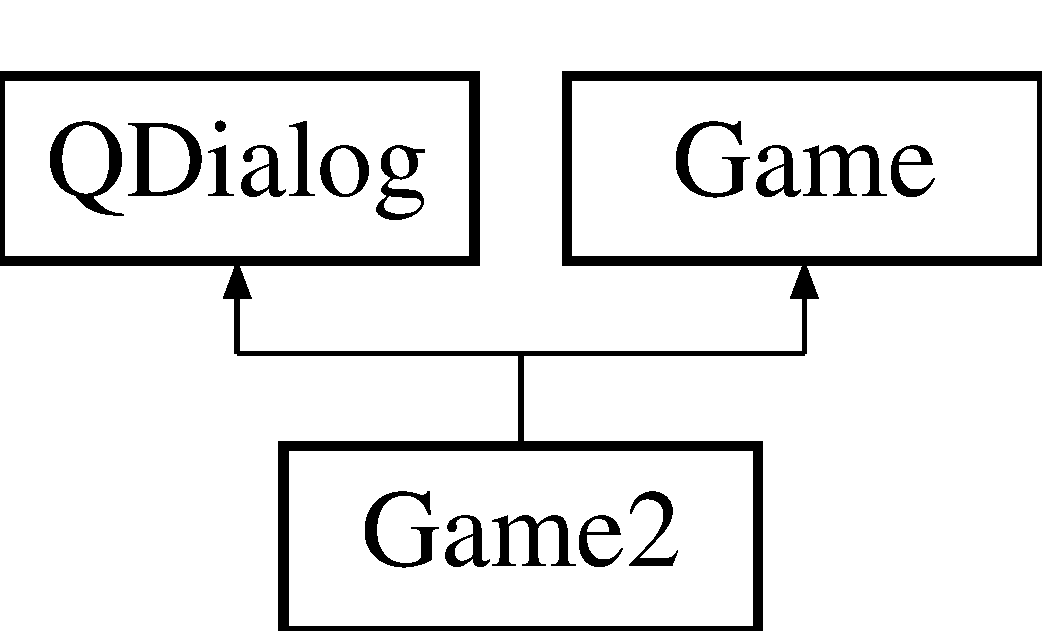
\includegraphics[height=2.000000cm]{classGame2}
\end{center}
\end{figure}
\subsection*{Public Member Functions}
\begin{DoxyCompactItemize}
\item 
\hypertarget{classGame2_acf087c1caa149631a1a20be7d90c8577}{{\bfseries Game2} (Q\-Widget $\ast$parent=0, \hyperlink{classUser}{User} $\ast$user=new \hyperlink{classUser}{User}())}\label{classGame2_acf087c1caa149631a1a20be7d90c8577}

\item 
\hypertarget{classGame2_a7c8c6d11b9f40a3cf3cc5b87f9a85807}{\hyperlink{classGame2_a7c8c6d11b9f40a3cf3cc5b87f9a85807}{$\sim$\-Game2} ()}\label{classGame2_a7c8c6d11b9f40a3cf3cc5b87f9a85807}

\begin{DoxyCompactList}\small\item\em destructor \end{DoxyCompactList}\end{DoxyCompactItemize}
\subsection*{Static Public Attributes}
\begin{DoxyCompactItemize}
\item 
\hypertarget{classGame2_a86faa987733f5a4b264d3f964261ffe9}{static Q\-String {\bfseries name} = \char`\"{}Game2\char`\"{}}\label{classGame2_a86faa987733f5a4b264d3f964261ffe9}

\end{DoxyCompactItemize}
\subsection*{Additional Inherited Members}


The documentation for this class was generated from the following files\-:\begin{DoxyCompactItemize}
\item 
game2.\-h\item 
\hyperlink{game2_8cpp}{game2.\-cpp}\end{DoxyCompactItemize}

\hypertarget{classGame2Scene}{\section{Game2\-Scene Class Reference}
\label{classGame2Scene}\index{Game2\-Scene@{Game2\-Scene}}
}


\hyperlink{classGame2Scene}{Game2\-Scene} class.  




{\ttfamily \#include $<$game2scene.\-h$>$}

Inheritance diagram for Game2\-Scene\-:\begin{figure}[H]
\begin{center}
\leavevmode
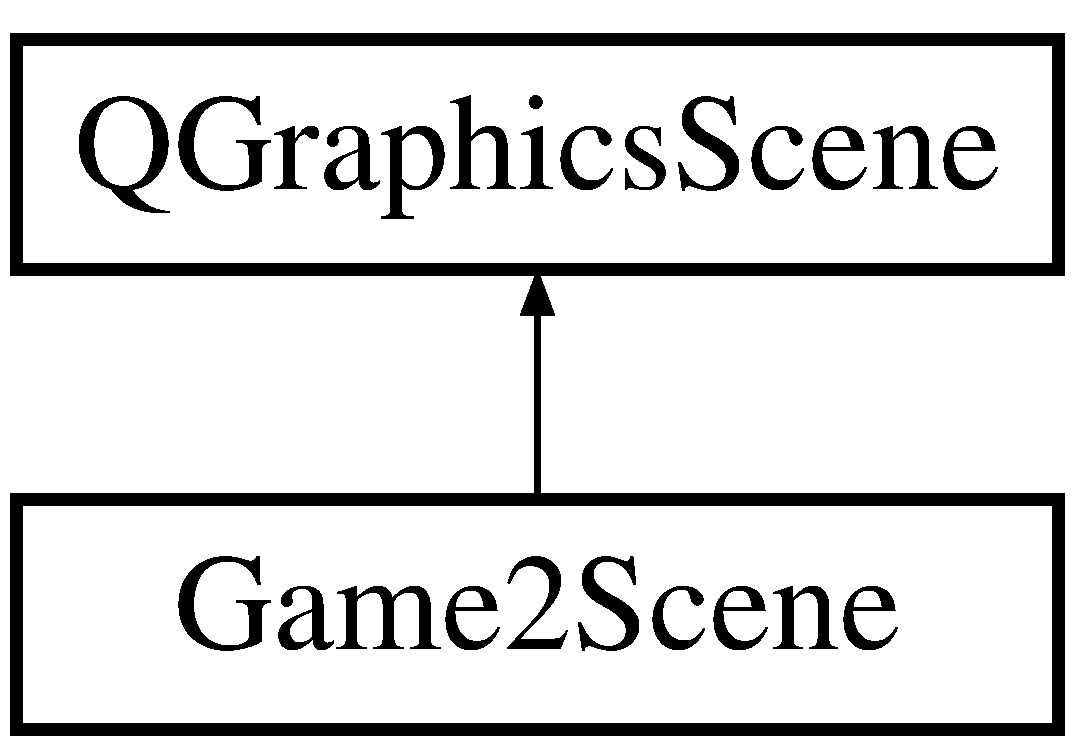
\includegraphics[height=2.000000cm]{classGame2Scene}
\end{center}
\end{figure}
\subsection*{Public Slots}
\begin{DoxyCompactItemize}
\item 
void \hyperlink{classGame2Scene_a7d832a1e88a9f6205dc58c806f118ecd}{addhu\-Items} ()
\begin{DoxyCompactList}\small\item\em add hu\-Items on the screen \end{DoxyCompactList}\item 
\hypertarget{classGame2Scene_a7a0475c2a2578482c27d04bc90499c6e}{void {\bfseries Close\-View} ()}\label{classGame2Scene_a7a0475c2a2578482c27d04bc90499c6e}

\end{DoxyCompactItemize}
\subsection*{Public Member Functions}
\begin{DoxyCompactItemize}
\item 
\hyperlink{classGame2Scene_a3e7775376b16bb0e7870b4a4ebe50b06}{Game2\-Scene} (\hyperlink{classGameView}{Game\-View} $\ast$game\-View, int game\-Mode, Q\-String username, int difficulty=1, \hyperlink{classHeader}{Header} $\ast$\hyperlink{classGame2Scene_ab20468619c00df91ed73eb1cce3ce5cf}{header}=nullptr, bool paused=false)
\begin{DoxyCompactList}\small\item\em constructor \end{DoxyCompactList}\item 
\hypertarget{classGame2Scene_a244be25736db0fe9b4525c627e2a5927}{void \hyperlink{classGame2Scene_a244be25736db0fe9b4525c627e2a5927}{Game\-Over} ()}\label{classGame2Scene_a244be25736db0fe9b4525c627e2a5927}

\begin{DoxyCompactList}\small\item\em \hyperlink{classGame2Scene_a244be25736db0fe9b4525c627e2a5927}{Game2\-Scene\-::\-Game\-Over} this is excited when a player looses the game. \end{DoxyCompactList}\item 
void \hyperlink{classGame2Scene_a74ad2a4ef08b8bfed2b2634c6da803c8}{Won\-Game} ()
\begin{DoxyCompactList}\small\item\em \hyperlink{classGame2Scene_a74ad2a4ef08b8bfed2b2634c6da803c8}{Game2\-Scene\-::\-Won\-Game} this is excited when a player wins the game. \end{DoxyCompactList}\item 
void \hyperlink{classGame2Scene_a5016fa1e0f3dae92ef399f35aae368f3}{Pause\-Game} ()
\begin{DoxyCompactList}\small\item\em \hyperlink{classGame2Scene_a5016fa1e0f3dae92ef399f35aae368f3}{Game2\-Scene\-::\-Pause\-Game} this is excited when a player pauses the game. \end{DoxyCompactList}\item 
\hypertarget{classGame2Scene_ac9de3cff4a4c70508704cfc331b95b73}{void {\bfseries key\-Press\-Event} (Q\-Key\-Event $\ast$event)}\label{classGame2Scene_ac9de3cff4a4c70508704cfc331b95b73}

\item 
void \hyperlink{classGame2Scene_ae876b70229a171d135daef2dcc6cd7ac}{key\-Release\-Event} (Q\-Key\-Event $\ast$event)
\begin{DoxyCompactList}\small\item\em Detects key release events. \end{DoxyCompactList}\item 
void \hyperlink{classGame2Scene_a0150f2992b0229a27d6d9852f4e5e7d3}{mouse\-Release\-Event} (Q\-Graphics\-Scene\-Mouse\-Event $\ast$event)
\begin{DoxyCompactList}\small\item\em \hyperlink{classGame2Scene_a0150f2992b0229a27d6d9852f4e5e7d3}{Game2\-Scene\-::mouse\-Release\-Event}. \end{DoxyCompactList}\item 
\hypertarget{classGame2Scene_afb89d017cdab6ebf2c7224803fb88d2b}{\hyperlink{classGame2Scene_afb89d017cdab6ebf2c7224803fb88d2b}{$\sim$\-Game2\-Scene} ()}\label{classGame2Scene_afb89d017cdab6ebf2c7224803fb88d2b}

\begin{DoxyCompactList}\small\item\em destructor \end{DoxyCompactList}\end{DoxyCompactItemize}
\subsection*{Public Attributes}
\begin{DoxyCompactItemize}
\item 
\hypertarget{classGame2Scene_ab20468619c00df91ed73eb1cce3ce5cf}{\hyperlink{classHeader}{Header} $\ast$ \hyperlink{classGame2Scene_ab20468619c00df91ed73eb1cce3ce5cf}{header}}\label{classGame2Scene_ab20468619c00df91ed73eb1cce3ce5cf}

\begin{DoxyCompactList}\small\item\em pointer to header \end{DoxyCompactList}\item 
\hypertarget{classGame2Scene_aae652a43bd3057bdeaec0a058aa47549}{Q\-Timer $\ast$ \hyperlink{classGame2Scene_aae652a43bd3057bdeaec0a058aa47549}{add\-Item\-To\-Queue\-Timer}}\label{classGame2Scene_aae652a43bd3057bdeaec0a058aa47549}

\begin{DoxyCompactList}\small\item\em Q\-Timer attribute,. \end{DoxyCompactList}\item 
\hypertarget{classGame2Scene_afded2510186d15031dc9099375d26769}{\hyperlink{classGameView}{Game\-View} $\ast$ {\bfseries game\-View}}\label{classGame2Scene_afded2510186d15031dc9099375d26769}

\item 
\hypertarget{classGame2Scene_a124c98a6c77d9fc892dda3b87bf9476f}{bool {\bfseries paused}}\label{classGame2Scene_a124c98a6c77d9fc892dda3b87bf9476f}

\item 
\hypertarget{classGame2Scene_a4ec4e660c6fe95e0fd328cf5648fd5ec}{bool {\bfseries completed}}\label{classGame2Scene_a4ec4e660c6fe95e0fd328cf5648fd5ec}

\end{DoxyCompactItemize}


\subsection{Detailed Description}
\hyperlink{classGame2Scene}{Game2\-Scene} class. 

.h This creates an instance of \hyperlink{classGame2Scene}{Game2\-Scene} which includes a spongebob and other items. 

\subsection{Constructor \& Destructor Documentation}
\hypertarget{classGame2Scene_a3e7775376b16bb0e7870b4a4ebe50b06}{\index{Game2\-Scene@{Game2\-Scene}!Game2\-Scene@{Game2\-Scene}}
\index{Game2\-Scene@{Game2\-Scene}!Game2Scene@{Game2\-Scene}}
\subsubsection[{Game2\-Scene}]{\setlength{\rightskip}{0pt plus 5cm}Game2\-Scene\-::\-Game2\-Scene (
\begin{DoxyParamCaption}
\item[{{\bf Game\-View} $\ast$}]{game\-View, }
\item[{int}]{game\-Mode, }
\item[{Q\-String}]{username, }
\item[{int}]{difficulty = {\ttfamily 1}, }
\item[{{\bf Header} $\ast$}]{header = {\ttfamily nullptr}, }
\item[{bool}]{paused = {\ttfamily false}}
\end{DoxyParamCaption}
)\hspace{0.3cm}{\ttfamily [explicit]}}}\label{classGame2Scene_a3e7775376b16bb0e7870b4a4ebe50b06}


constructor 

\hyperlink{classGame2Scene_a3e7775376b16bb0e7870b4a4ebe50b06}{Game2\-Scene\-::\-Game2\-Scene} constructs the \hyperlink{classGame2Scene}{Game2\-Scene} and all of its attributes, starts the timers, and connects the signal with its slot. player lost the game

player won the game

the game is being paused

starting a new game

resuming from a paused game 

\subsection{Member Function Documentation}
\hypertarget{classGame2Scene_a7d832a1e88a9f6205dc58c806f118ecd}{\index{Game2\-Scene@{Game2\-Scene}!addhu\-Items@{addhu\-Items}}
\index{addhu\-Items@{addhu\-Items}!Game2Scene@{Game2\-Scene}}
\subsubsection[{addhu\-Items}]{\setlength{\rightskip}{0pt plus 5cm}void Game2\-Scene\-::addhu\-Items (
\begin{DoxyParamCaption}
{}
\end{DoxyParamCaption}
)\hspace{0.3cm}{\ttfamily [slot]}}}\label{classGame2Scene_a7d832a1e88a9f6205dc58c806f118ecd}


add hu\-Items on the screen 

\hyperlink{classGame2Scene_a7d832a1e88a9f6205dc58c806f118ecd}{Game2\-Scene\-::addhu\-Items} this function is responsible for adding healthy/unhealthy items to the screen.

healty/unhealthy ratio is determined by the gmae difficulty where a ratio of 3\-:1 is used for the easy level, and a 1\-:3 is used for the hard one the image of the healthy or unhealthy item is also spceified randomly from 4 pictures for each type. first number (0 or1) is for type of item (1 is healthy and 0 is unhealthy) the second is for the picture to display \hypertarget{classGame2Scene_ae876b70229a171d135daef2dcc6cd7ac}{\index{Game2\-Scene@{Game2\-Scene}!key\-Release\-Event@{key\-Release\-Event}}
\index{key\-Release\-Event@{key\-Release\-Event}!Game2Scene@{Game2\-Scene}}
\subsubsection[{key\-Release\-Event}]{\setlength{\rightskip}{0pt plus 5cm}void Game2\-Scene\-::key\-Release\-Event (
\begin{DoxyParamCaption}
\item[{Q\-Key\-Event $\ast$}]{event}
\end{DoxyParamCaption}
)}}\label{classGame2Scene_ae876b70229a171d135daef2dcc6cd7ac}


Detects key release events. 

\hyperlink{classGame2Scene_ae876b70229a171d135daef2dcc6cd7ac}{Game2\-Scene\-::key\-Release\-Event}.


\begin{DoxyParams}{Parameters}
{\em $\ast$event} & first argument, key release event\\
\hline
{\em event} & this collects key release events and removes them from the set of pressed keys \\
\hline
\end{DoxyParams}
\hypertarget{classGame2Scene_a0150f2992b0229a27d6d9852f4e5e7d3}{\index{Game2\-Scene@{Game2\-Scene}!mouse\-Release\-Event@{mouse\-Release\-Event}}
\index{mouse\-Release\-Event@{mouse\-Release\-Event}!Game2Scene@{Game2\-Scene}}
\subsubsection[{mouse\-Release\-Event}]{\setlength{\rightskip}{0pt plus 5cm}void Game2\-Scene\-::mouse\-Release\-Event (
\begin{DoxyParamCaption}
\item[{Q\-Graphics\-Scene\-Mouse\-Event $\ast$}]{event}
\end{DoxyParamCaption}
)}}\label{classGame2Scene_a0150f2992b0229a27d6d9852f4e5e7d3}


\hyperlink{classGame2Scene_a0150f2992b0229a27d6d9852f4e5e7d3}{Game2\-Scene\-::mouse\-Release\-Event}. 


\begin{DoxyParams}{Parameters}
{\em event} & this detects the mouse release event in order to pause the game \\
\hline
\end{DoxyParams}
\hypertarget{classGame2Scene_a5016fa1e0f3dae92ef399f35aae368f3}{\index{Game2\-Scene@{Game2\-Scene}!Pause\-Game@{Pause\-Game}}
\index{Pause\-Game@{Pause\-Game}!Game2Scene@{Game2\-Scene}}
\subsubsection[{Pause\-Game}]{\setlength{\rightskip}{0pt plus 5cm}void Game2\-Scene\-::\-Pause\-Game (
\begin{DoxyParamCaption}
{}
\end{DoxyParamCaption}
)}}\label{classGame2Scene_a5016fa1e0f3dae92ef399f35aae368f3}


\hyperlink{classGame2Scene_a5016fa1e0f3dae92ef399f35aae368f3}{Game2\-Scene\-::\-Pause\-Game} this is excited when a player pauses the game. 

the player metrics (score, timer, number of lives...) are saved to be retreived on the resume. if the player is a registered one, his metrics are also stored in the game database for later retreval. else wise, his metrics are saved as long as the game window is not closed. \hypertarget{classGame2Scene_a74ad2a4ef08b8bfed2b2634c6da803c8}{\index{Game2\-Scene@{Game2\-Scene}!Won\-Game@{Won\-Game}}
\index{Won\-Game@{Won\-Game}!Game2Scene@{Game2\-Scene}}
\subsubsection[{Won\-Game}]{\setlength{\rightskip}{0pt plus 5cm}void Game2\-Scene\-::\-Won\-Game (
\begin{DoxyParamCaption}
{}
\end{DoxyParamCaption}
)}}\label{classGame2Scene_a74ad2a4ef08b8bfed2b2634c6da803c8}


\hyperlink{classGame2Scene_a74ad2a4ef08b8bfed2b2634c6da803c8}{Game2\-Scene\-::\-Won\-Game} this is excited when a player wins the game. 

if the player is a registered one ( not a guest), his score is added to his history of scores. additionally, winning a game would allow the user to play a higher level. 

The documentation for this class was generated from the following files\-:\begin{DoxyCompactItemize}
\item 
game2scene.\-h\item 
game2scene.\-cpp\end{DoxyCompactItemize}

\hypertarget{classGamemenu}{\section{Gamemenu Class Reference}
\label{classGamemenu}\index{Gamemenu@{Gamemenu}}
}
Inheritance diagram for Gamemenu\-:\begin{figure}[H]
\begin{center}
\leavevmode
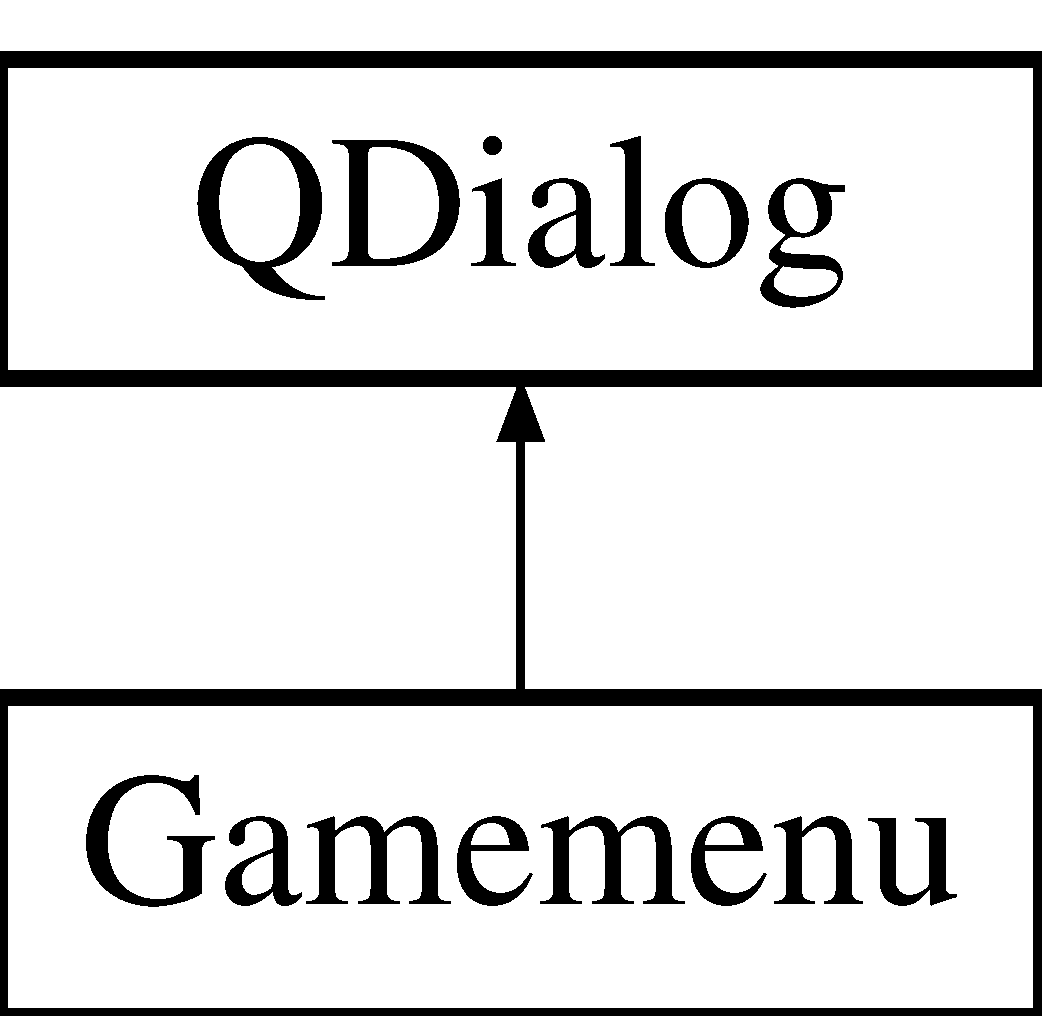
\includegraphics[height=2.000000cm]{classGamemenu}
\end{center}
\end{figure}
\subsection*{Public Member Functions}
\begin{DoxyCompactItemize}
\item 
\hypertarget{classGamemenu_a93a8b2e28dae56b3bededa8aa0727fa5}{{\bfseries Gamemenu} (Q\-Widget $\ast$parent=0, Q\-String game=\char`\"{}\char`\"{}, \hyperlink{classUser}{User} $\ast$user=new \hyperlink{classUser}{User}())}\label{classGamemenu_a93a8b2e28dae56b3bededa8aa0727fa5}

\item 
\hypertarget{classGamemenu_a3ed45d70a8f2fb73ca5900252a350ff1}{\hyperlink{classGamemenu_a3ed45d70a8f2fb73ca5900252a350ff1}{$\sim$\-Gamemenu} ()}\label{classGamemenu_a3ed45d70a8f2fb73ca5900252a350ff1}

\begin{DoxyCompactList}\small\item\em destructor \end{DoxyCompactList}\end{DoxyCompactItemize}
\subsection*{Public Attributes}
\begin{DoxyCompactItemize}
\item 
\hypertarget{classGamemenu_ae931024c5e37bbbb5776a81461597939}{Q\-String {\bfseries Game}}\label{classGamemenu_ae931024c5e37bbbb5776a81461597939}

\item 
\hypertarget{classGamemenu_a44560505e0acfb662c0438e58b15bf94}{\hyperlink{classUser}{User} $\ast$ {\bfseries user}}\label{classGamemenu_a44560505e0acfb662c0438e58b15bf94}

\end{DoxyCompactItemize}


The documentation for this class was generated from the following files\-:\begin{DoxyCompactItemize}
\item 
gamemenu.\-h\item 
\hyperlink{gamemenu_8cpp}{gamemenu.\-cpp}\end{DoxyCompactItemize}

\hypertarget{classGameView}{\section{Game\-View Class Reference}
\label{classGameView}\index{Game\-View@{Game\-View}}
}
Inheritance diagram for Game\-View\-:\begin{figure}[H]
\begin{center}
\leavevmode
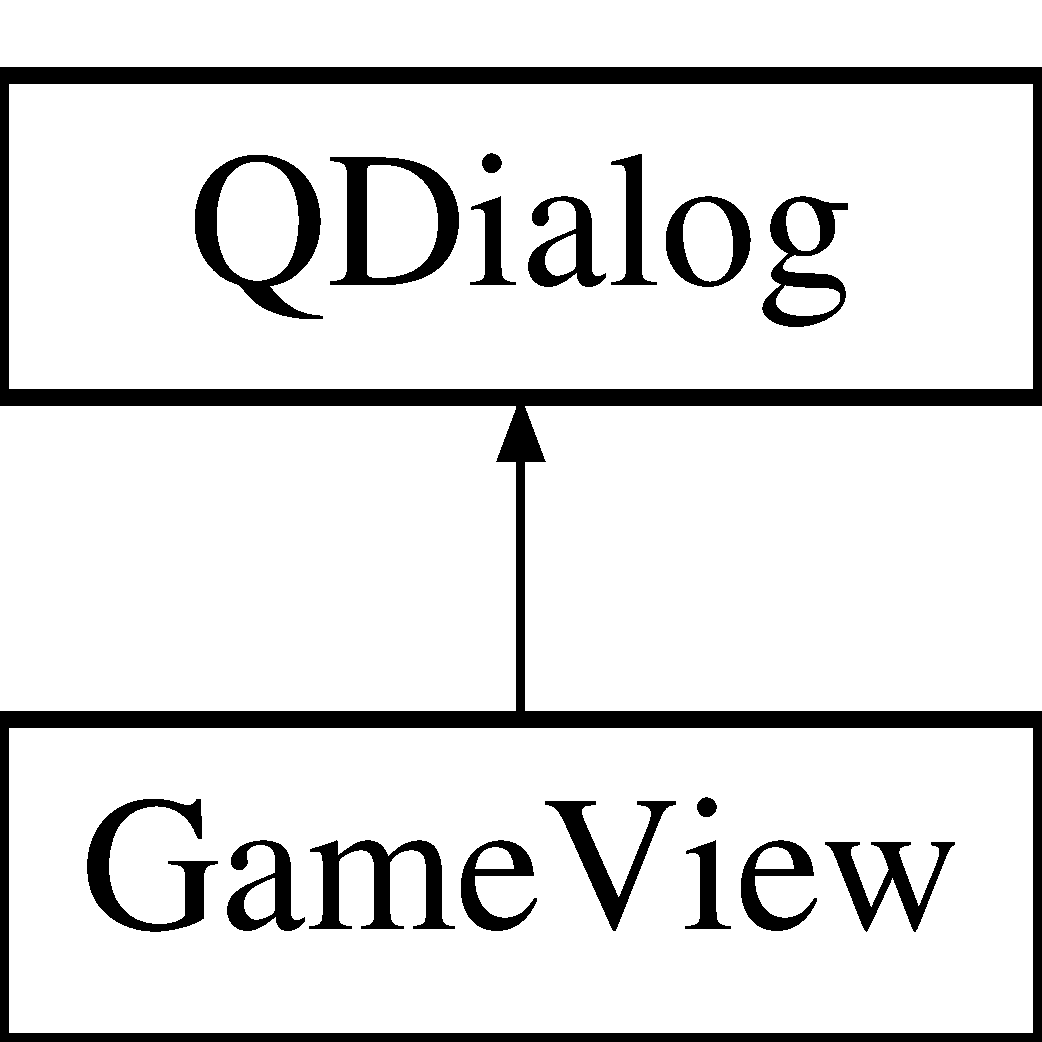
\includegraphics[height=2.000000cm]{classGameView}
\end{center}
\end{figure}
\subsection*{Public Member Functions}
\begin{DoxyCompactItemize}
\item 
\hypertarget{classGameView_a6f41d09f51d2abd6abb3b99e5da8ef6f}{{\bfseries Game\-View} (Q\-Widget $\ast$parent=0)}\label{classGameView_a6f41d09f51d2abd6abb3b99e5da8ef6f}

\item 
\hypertarget{classGameView_a99555fe40cf367386272760cfd5ffd82}{void \hyperlink{classGameView_a99555fe40cf367386272760cfd5ffd82}{set\-Scene} (Q\-Graphics\-Scene $\ast$game\-Scene)}\label{classGameView_a99555fe40cf367386272760cfd5ffd82}

\begin{DoxyCompactList}\small\item\em creating the scene ( game 1 or 2), and centering the game in the middle of the screen. \end{DoxyCompactList}\end{DoxyCompactItemize}
\subsection*{Public Attributes}
\begin{DoxyCompactItemize}
\item 
\hypertarget{classGameView_a268225b0de88730c884f0deffc85059a}{Q\-Graphics\-Scene $\ast$ {\bfseries game\-Scene}}\label{classGameView_a268225b0de88730c884f0deffc85059a}

\end{DoxyCompactItemize}


The documentation for this class was generated from the following files\-:\begin{DoxyCompactItemize}
\item 
gameview.\-h\item 
\hyperlink{gameview_8cpp}{gameview.\-cpp}\end{DoxyCompactItemize}

\hypertarget{classGrabbable}{\section{Grabbable Class Reference}
\label{classGrabbable}\index{Grabbable@{Grabbable}}
}
Inheritance diagram for Grabbable\-:\begin{figure}[H]
\begin{center}
\leavevmode
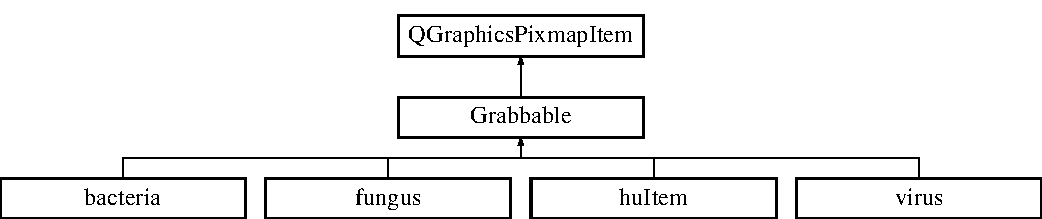
\includegraphics[height=2.937063cm]{classGrabbable}
\end{center}
\end{figure}
\subsection*{Public Member Functions}
\begin{DoxyCompactItemize}
\item 
void \hyperlink{classGrabbable_a54abafe482bfeff9bc4950eb1af86729}{was\-Grabbed} ()
\begin{DoxyCompactList}\small\item\em \hyperlink{classGrabbable_a54abafe482bfeff9bc4950eb1af86729}{Grabbable\-::was\-Grabbed} this function is excited when an item is hooked. \end{DoxyCompactList}\item 
void \hyperlink{classGrabbable_a1dbbee1086ee34f1c32493a7c80e0f04}{was\-Shot} (\hyperlink{classWeapon}{Weapon} $\ast$by)
\begin{DoxyCompactList}\small\item\em excited when an item is shot ( laser or bomb) \end{DoxyCompactList}\item 
void \hyperlink{classGrabbable_ab6352505d07da9d327be2f74faaae141}{reached\-Baby} ()
\begin{DoxyCompactList}\small\item\em \hyperlink{classGrabbable_ab6352505d07da9d327be2f74faaae141}{Grabbable\-::reached\-Baby} this is a function that is excited when the baby collides with an item. \end{DoxyCompactList}\end{DoxyCompactItemize}
\subsection*{Public Attributes}
\begin{DoxyCompactItemize}
\item 
\hypertarget{classGrabbable_a97db8193dec83a8086352f80a30b2038}{\hyperlink{classHeader}{Header} $\ast$ \hyperlink{classGrabbable_a97db8193dec83a8086352f80a30b2038}{header}}\label{classGrabbable_a97db8193dec83a8086352f80a30b2038}

\begin{DoxyCompactList}\small\item\em pointer to the header \end{DoxyCompactList}\item 
\hypertarget{classGrabbable_a161e54edc1ba06f3f9d3724c52ffa479}{int {\bfseries strength}}\label{classGrabbable_a161e54edc1ba06f3f9d3724c52ffa479}

\item 
\hypertarget{classGrabbable_ad6afb7dae68be483e218d380b763e03e}{int {\bfseries interval}}\label{classGrabbable_ad6afb7dae68be483e218d380b763e03e}

\item 
\hypertarget{classGrabbable_a055aa96768fbbcf9ef6e5154594f0e39}{bool {\bfseries grabbed}}\label{classGrabbable_a055aa96768fbbcf9ef6e5154594f0e39}

\end{DoxyCompactItemize}


\subsection{Member Function Documentation}
\hypertarget{classGrabbable_ab6352505d07da9d327be2f74faaae141}{\index{Grabbable@{Grabbable}!reached\-Baby@{reached\-Baby}}
\index{reached\-Baby@{reached\-Baby}!Grabbable@{Grabbable}}
\subsubsection[{reached\-Baby}]{\setlength{\rightskip}{0pt plus 5cm}void Grabbable\-::reached\-Baby (
\begin{DoxyParamCaption}
{}
\end{DoxyParamCaption}
)}}\label{classGrabbable_ab6352505d07da9d327be2f74faaae141}


\hyperlink{classGrabbable_ab6352505d07da9d327be2f74faaae141}{Grabbable\-::reached\-Baby} this is a function that is excited when the baby collides with an item. 

checking if the item collided with is an huitem.

if the huitem is an unhealthy item, the player loses a life.

if the huitem is a healthy item, the cleanliness increases.

removing the item that collided with the baby. \hypertarget{classGrabbable_a54abafe482bfeff9bc4950eb1af86729}{\index{Grabbable@{Grabbable}!was\-Grabbed@{was\-Grabbed}}
\index{was\-Grabbed@{was\-Grabbed}!Grabbable@{Grabbable}}
\subsubsection[{was\-Grabbed}]{\setlength{\rightskip}{0pt plus 5cm}void Grabbable\-::was\-Grabbed (
\begin{DoxyParamCaption}
{}
\end{DoxyParamCaption}
)}}\label{classGrabbable_a54abafe482bfeff9bc4950eb1af86729}


\hyperlink{classGrabbable_a54abafe482bfeff9bc4950eb1af86729}{Grabbable\-::was\-Grabbed} this function is excited when an item is hooked. 

adding or subtracting time and immunity based on the type of the grabbed item \hypertarget{classGrabbable_a1dbbee1086ee34f1c32493a7c80e0f04}{\index{Grabbable@{Grabbable}!was\-Shot@{was\-Shot}}
\index{was\-Shot@{was\-Shot}!Grabbable@{Grabbable}}
\subsubsection[{was\-Shot}]{\setlength{\rightskip}{0pt plus 5cm}void Grabbable\-::was\-Shot (
\begin{DoxyParamCaption}
\item[{{\bf Weapon} $\ast$}]{by}
\end{DoxyParamCaption}
)}}\label{classGrabbable_a1dbbee1086ee34f1c32493a7c80e0f04}


excited when an item is shot ( laser or bomb) 

if the item collides with a bomb, it loses all of its strength

if the item was shot with a laser, its strength decreases by the strength of the laser

if this is a healthy item, increase score.

if this is an unhealthy item, decrease score. 

The documentation for this class was generated from the following files\-:\begin{DoxyCompactItemize}
\item 
grabbable.\-h\item 
\hyperlink{grabbable_8cpp}{grabbable.\-cpp}\end{DoxyCompactItemize}

\hypertarget{classHeader}{\section{Header Class Reference}
\label{classHeader}\index{Header@{Header}}
}
Inheritance diagram for Header\-:\begin{figure}[H]
\begin{center}
\leavevmode
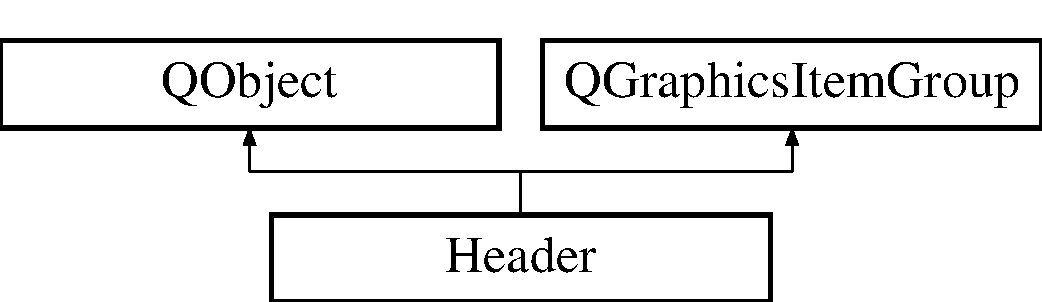
\includegraphics[height=2.000000cm]{classHeader}
\end{center}
\end{figure}
\subsection*{Public Slots}
\begin{DoxyCompactItemize}
\item 
\hypertarget{classHeader_a427b5d03b37b2f1bca1c5905447f42df}{void {\bfseries Count\-Down} ()}\label{classHeader_a427b5d03b37b2f1bca1c5905447f42df}

\end{DoxyCompactItemize}
\subsection*{Public Member Functions}
\begin{DoxyCompactItemize}
\item 
\hyperlink{classHeader_aa3cc08748158b541569bdd03649e62ff}{Header} (\hyperlink{classSpongeBob}{Sponge\-Bob} $\ast$player, int difficulty, Q\-String username, Q\-String game, bool paused, int time, int healthy\-Items\-Fed=0)
\item 
void \hyperlink{classHeader_a0a9d3d93d2a79b79ef29edfa1d5bdac2}{Set\-Cleanliness} (int val)
\begin{DoxyCompactList}\small\item\em \hyperlink{classHeader_a0a9d3d93d2a79b79ef29edfa1d5bdac2}{Header\-::\-Set\-Cleanliness}. \end{DoxyCompactList}\item 
void \hyperlink{classHeader_aa99fe86fab6bfe26278e186ba8426d2b}{Set\-Immunity} (int val)
\begin{DoxyCompactList}\small\item\em \hyperlink{classHeader_aa99fe86fab6bfe26278e186ba8426d2b}{Header\-::\-Set\-Immunity}. \end{DoxyCompactList}\item 
void \hyperlink{classHeader_aca556237518231a45ec6f7333d1f1631}{Set\-Score} (int val)
\item 
\hypertarget{classHeader_a8a2130ccbe80b5c1c6b980d63b3ad5fd}{void {\bfseries Set\-Time} (int val)}\label{classHeader_a8a2130ccbe80b5c1c6b980d63b3ad5fd}

\item 
\hypertarget{classHeader_acbb8865a147989d7da5cc2d57b5f5d03}{void {\bfseries Remove\-Life} ()}\label{classHeader_acbb8865a147989d7da5cc2d57b5f5d03}

\item 
\hypertarget{classHeader_ad5f7808b4a879f8a0b9fe1f6b07c59f9}{void {\bfseries Remove\-Bomb} ()}\label{classHeader_ad5f7808b4a879f8a0b9fe1f6b07c59f9}

\item 
void \hyperlink{classHeader_a715193e0d8b55c16fe7c205cd347ac5a}{Add\-Cleanl\-Meter} (int x, int y)
\begin{DoxyCompactList}\small\item\em \hyperlink{classHeader_a715193e0d8b55c16fe7c205cd347ac5a}{Header\-::\-Add\-Cleanl\-Meter}. \end{DoxyCompactList}\item 
\hypertarget{classHeader_a541c329b4ba77a9ab3004c23b43d1d76}{void {\bfseries Add\-Chart} (int x, int y, int width, int height, int start\-Angle, int span\-Angle, Q\-Color color)}\label{classHeader_a541c329b4ba77a9ab3004c23b43d1d76}

\item 
\hypertarget{classHeader_a0fac13736d7e8e507c329610843cb69c}{void {\bfseries Add\-Hearts} (int x, int y)}\label{classHeader_a0fac13736d7e8e507c329610843cb69c}

\item 
\hypertarget{classHeader_ae1f122fb7729e9930ab8476f5515a553}{void {\bfseries Add\-Time} (int x, int y)}\label{classHeader_ae1f122fb7729e9930ab8476f5515a553}

\item 
\hypertarget{classHeader_af8bb49d54827ccc10848225f1fbf4f4b}{void {\bfseries Add\-Pause} (int x, int y)}\label{classHeader_af8bb49d54827ccc10848225f1fbf4f4b}

\item 
\hypertarget{classHeader_a689b3d9320ab2541a21c402a5faf98d1}{void {\bfseries Add\-Level} (int x, int y)}\label{classHeader_a689b3d9320ab2541a21c402a5faf98d1}

\item 
\hypertarget{classHeader_ad70bb097047f2e6929f0b877e3c8313d}{void {\bfseries Add\-Score} (int x, int y)}\label{classHeader_ad70bb097047f2e6929f0b877e3c8313d}

\item 
void \hyperlink{classHeader_aa035a6e33a0a098e31f30847af6cfab5}{Add\-Needle} (int x, int y)
\begin{DoxyCompactList}\small\item\em \hyperlink{classHeader_aa035a6e33a0a098e31f30847af6cfab5}{Header\-::\-Add\-Needle}. \end{DoxyCompactList}\item 
\hypertarget{classHeader_a23c18703ab45ddb0433f04a4a458e70c}{void {\bfseries Add\-Baby} (int x, int y, int healthy\-Items\-Fed)}\label{classHeader_a23c18703ab45ddb0433f04a4a458e70c}

\item 
void \hyperlink{classHeader_a21be452fa582357209fba40253628e67}{Add\-Bombs} (int x, int y)
\begin{DoxyCompactList}\small\item\em \hyperlink{classHeader_a21be452fa582357209fba40253628e67}{Header\-::\-Add\-Bombs}. \end{DoxyCompactList}\item 
\hypertarget{classHeader_a2f60a58e7438f57e33780e1047e4b9ba}{void {\bfseries Add\-Score\-Calculation} (int x, int y)}\label{classHeader_a2f60a58e7438f57e33780e1047e4b9ba}

\item 
void \hyperlink{classHeader_ae84e230bd170c5019cf75a6aae297401}{Render} ()
\begin{DoxyCompactList}\small\item\em \hyperlink{classHeader_ae84e230bd170c5019cf75a6aae297401}{Header\-::\-Render} this is the main function for the visual representation of the updates of the metrics. \end{DoxyCompactList}\end{DoxyCompactItemize}
\subsection*{Public Attributes}
\begin{DoxyCompactItemize}
\item 
\hypertarget{classHeader_a54be6087baca716a9292e5167fe202a6}{\hyperlink{classCleanlinessMeter}{Cleanliness\-Meter} $\ast$ {\bfseries cleanliness\-Meter}}\label{classHeader_a54be6087baca716a9292e5167fe202a6}

\item 
\hypertarget{classHeader_a553e85cea35e1741289a29d4be789030}{\hyperlink{classPause}{Pause} $\ast$ {\bfseries pause}}\label{classHeader_a553e85cea35e1741289a29d4be789030}

\item 
\hypertarget{classHeader_a4ee68fceb0cc90edfdbc60d22337cc1d}{Q\-Graphics\-Pixmap\-Item $\ast$ {\bfseries hearts} \mbox{[}3\mbox{]}}\label{classHeader_a4ee68fceb0cc90edfdbc60d22337cc1d}

\item 
\hypertarget{classHeader_a7464258724785cc5a337c1dfffc31c77}{Q\-Graphics\-Pixmap\-Item $\ast$ {\bfseries bombs} \mbox{[}3\mbox{]}}\label{classHeader_a7464258724785cc5a337c1dfffc31c77}

\item 
\hypertarget{classHeader_a934ddf4ece375a0e6f6c36ca6dd83976}{Q\-Graphics\-Text\-Item $\ast$ {\bfseries time\-Label}}\label{classHeader_a934ddf4ece375a0e6f6c36ca6dd83976}

\item 
\hypertarget{classHeader_aca0e61105e8794506e30b8ff6ac12e04}{Q\-Graphics\-Text\-Item $\ast$ {\bfseries level\-Label}}\label{classHeader_aca0e61105e8794506e30b8ff6ac12e04}

\item 
\hypertarget{classHeader_a5f9ab3bc1db27b933956d26b6209e031}{Q\-Graphics\-Text\-Item $\ast$ {\bfseries score\-Label}}\label{classHeader_a5f9ab3bc1db27b933956d26b6209e031}

\item 
\hypertarget{classHeader_ade38e66c5f7ce36035160c231f39e322}{Q\-Graphics\-Text\-Item $\ast$ {\bfseries score\-Calculation\-Label}}\label{classHeader_ade38e66c5f7ce36035160c231f39e322}

\item 
\hypertarget{classHeader_ab974256995a71056eb97c8018246d8e2}{Q\-Graphics\-Line\-Item $\ast$ {\bfseries needle}}\label{classHeader_ab974256995a71056eb97c8018246d8e2}

\item 
\hypertarget{classHeader_a85ac821bfce84ceb3978d65f53e2b558}{\hyperlink{classSpongeBob}{Sponge\-Bob} $\ast$ {\bfseries player}}\label{classHeader_a85ac821bfce84ceb3978d65f53e2b558}

\item 
\hypertarget{classHeader_aedf088252280ab5eb09c73e5fd3517ad}{\hyperlink{classBabySpongeBob}{Baby\-Sponge\-Bob} $\ast$ {\bfseries baby}}\label{classHeader_aedf088252280ab5eb09c73e5fd3517ad}

\item 
\hypertarget{classHeader_ace92a7d778ae16edec96ff5c25fcf901}{Q\-String {\bfseries username}}\label{classHeader_ace92a7d778ae16edec96ff5c25fcf901}

\item 
\hypertarget{classHeader_a7f997858c1f7a9f88e50fcbf464a5d38}{Q\-String {\bfseries game}}\label{classHeader_a7f997858c1f7a9f88e50fcbf464a5d38}

\item 
\hypertarget{classHeader_a3322a706106c6a42600ae2acbd6fe155}{Q\-Timer $\ast$ {\bfseries timer}}\label{classHeader_a3322a706106c6a42600ae2acbd6fe155}

\item 
\hypertarget{classHeader_a44ca0ffcdf952bb61362f5a365f3a573}{int {\bfseries time}}\label{classHeader_a44ca0ffcdf952bb61362f5a365f3a573}

\item 
\hypertarget{classHeader_ac7d3698ffe7993f0153783a8dcd9bf2f}{int {\bfseries difficulty}}\label{classHeader_ac7d3698ffe7993f0153783a8dcd9bf2f}

\item 
\hypertarget{classHeader_a5b09994627054550891bce868d51cefb}{int {\bfseries current\-Bacteria\-Count\-In\-Scene}}\label{classHeader_a5b09994627054550891bce868d51cefb}

\item 
\hypertarget{classHeader_a9b351d1a7df2d6c40e96afe9a3d1d0d8}{int {\bfseries counter}}\label{classHeader_a9b351d1a7df2d6c40e96afe9a3d1d0d8}

\item 
\hypertarget{classHeader_a6523f2b63659afa3205a48e9805aed3b}{bool {\bfseries paused}}\label{classHeader_a6523f2b63659afa3205a48e9805aed3b}

\end{DoxyCompactItemize}


\subsection{Constructor \& Destructor Documentation}
\hypertarget{classHeader_aa3cc08748158b541569bdd03649e62ff}{\index{Header@{Header}!Header@{Header}}
\index{Header@{Header}!Header@{Header}}
\subsubsection[{Header}]{\setlength{\rightskip}{0pt plus 5cm}Header\-::\-Header (
\begin{DoxyParamCaption}
\item[{{\bf Sponge\-Bob} $\ast$}]{player, }
\item[{int}]{difficulty, }
\item[{Q\-String}]{username, }
\item[{Q\-String}]{game, }
\item[{bool}]{paused, }
\item[{int}]{time, }
\item[{int}]{healthy\-Items\-Fed = {\ttfamily 0}}
\end{DoxyParamCaption}
)}}\label{classHeader_aa3cc08748158b541569bdd03649e62ff}
setting metrics

setting graphics 

\subsection{Member Function Documentation}
\hypertarget{classHeader_a21be452fa582357209fba40253628e67}{\index{Header@{Header}!Add\-Bombs@{Add\-Bombs}}
\index{Add\-Bombs@{Add\-Bombs}!Header@{Header}}
\subsubsection[{Add\-Bombs}]{\setlength{\rightskip}{0pt plus 5cm}void Header\-::\-Add\-Bombs (
\begin{DoxyParamCaption}
\item[{int}]{x, }
\item[{int}]{y}
\end{DoxyParamCaption}
)}}\label{classHeader_a21be452fa582357209fba40253628e67}


\hyperlink{classHeader_a21be452fa582357209fba40253628e67}{Header\-::\-Add\-Bombs}. 


\begin{DoxyParams}{Parameters}
{\em x} & \\
\hline
{\em y} & this function adds bombs to the header of the game scene \\
\hline
\end{DoxyParams}
\hypertarget{classHeader_a715193e0d8b55c16fe7c205cd347ac5a}{\index{Header@{Header}!Add\-Cleanl\-Meter@{Add\-Cleanl\-Meter}}
\index{Add\-Cleanl\-Meter@{Add\-Cleanl\-Meter}!Header@{Header}}
\subsubsection[{Add\-Cleanl\-Meter}]{\setlength{\rightskip}{0pt plus 5cm}void Header\-::\-Add\-Cleanl\-Meter (
\begin{DoxyParamCaption}
\item[{int}]{x, }
\item[{int}]{y}
\end{DoxyParamCaption}
)}}\label{classHeader_a715193e0d8b55c16fe7c205cd347ac5a}


\hyperlink{classHeader_a715193e0d8b55c16fe7c205cd347ac5a}{Header\-::\-Add\-Cleanl\-Meter}. 


\begin{DoxyParams}{Parameters}
{\em x} & \\
\hline
{\em y} & adds the cleanliness meter to the scene, the position of the meter is set by the x and y coordinates \\
\hline
\end{DoxyParams}
\hypertarget{classHeader_aa035a6e33a0a098e31f30847af6cfab5}{\index{Header@{Header}!Add\-Needle@{Add\-Needle}}
\index{Add\-Needle@{Add\-Needle}!Header@{Header}}
\subsubsection[{Add\-Needle}]{\setlength{\rightskip}{0pt plus 5cm}void Header\-::\-Add\-Needle (
\begin{DoxyParamCaption}
\item[{int}]{x, }
\item[{int}]{y}
\end{DoxyParamCaption}
)}}\label{classHeader_aa035a6e33a0a098e31f30847af6cfab5}


\hyperlink{classHeader_aa035a6e33a0a098e31f30847af6cfab5}{Header\-::\-Add\-Needle}. 


\begin{DoxyParams}{Parameters}
{\em x} & \\
\hline
{\em y} & this function adds the needle to the chart in the header of the game. the needle acts as an indicator to the strength of the player \\
\hline
\end{DoxyParams}
\hypertarget{classHeader_ae84e230bd170c5019cf75a6aae297401}{\index{Header@{Header}!Render@{Render}}
\index{Render@{Render}!Header@{Header}}
\subsubsection[{Render}]{\setlength{\rightskip}{0pt plus 5cm}void Header\-::\-Render (
\begin{DoxyParamCaption}
{}
\end{DoxyParamCaption}
)}}\label{classHeader_ae84e230bd170c5019cf75a6aae297401}


\hyperlink{classHeader_ae84e230bd170c5019cf75a6aae297401}{Header\-::\-Render} this is the main function for the visual representation of the updates of the metrics. 

it is called when an update to a metric occures, and it updates accordingly the visual representation of the metrics in the header \hypertarget{classHeader_a0a9d3d93d2a79b79ef29edfa1d5bdac2}{\index{Header@{Header}!Set\-Cleanliness@{Set\-Cleanliness}}
\index{Set\-Cleanliness@{Set\-Cleanliness}!Header@{Header}}
\subsubsection[{Set\-Cleanliness}]{\setlength{\rightskip}{0pt plus 5cm}void Header\-::\-Set\-Cleanliness (
\begin{DoxyParamCaption}
\item[{int}]{val}
\end{DoxyParamCaption}
)}}\label{classHeader_a0a9d3d93d2a79b79ef29edfa1d5bdac2}


\hyperlink{classHeader_a0a9d3d93d2a79b79ef29edfa1d5bdac2}{Header\-::\-Set\-Cleanliness}. 


\begin{DoxyParams}{Parameters}
{\em val} & the val is added(or subtracted if negative) from the total cleanliness level if the level is less than 0 or greater than 100, the value is reseted to zero or 100 \\
\hline
\end{DoxyParams}
\hypertarget{classHeader_aa99fe86fab6bfe26278e186ba8426d2b}{\index{Header@{Header}!Set\-Immunity@{Set\-Immunity}}
\index{Set\-Immunity@{Set\-Immunity}!Header@{Header}}
\subsubsection[{Set\-Immunity}]{\setlength{\rightskip}{0pt plus 5cm}void Header\-::\-Set\-Immunity (
\begin{DoxyParamCaption}
\item[{int}]{val}
\end{DoxyParamCaption}
)}}\label{classHeader_aa99fe86fab6bfe26278e186ba8426d2b}


\hyperlink{classHeader_aa99fe86fab6bfe26278e186ba8426d2b}{Header\-::\-Set\-Immunity}. 


\begin{DoxyParams}{Parameters}
{\em val} & this sets the immunity by adding(or subtracting) the value of val from the current immmunity level \\
\hline
\end{DoxyParams}
\hypertarget{classHeader_aca556237518231a45ec6f7333d1f1631}{\index{Header@{Header}!Set\-Score@{Set\-Score}}
\index{Set\-Score@{Set\-Score}!Header@{Header}}
\subsubsection[{Set\-Score}]{\setlength{\rightskip}{0pt plus 5cm}void Header\-::\-Set\-Score (
\begin{DoxyParamCaption}
\item[{int}]{val}
\end{DoxyParamCaption}
)}}\label{classHeader_aca556237518231a45ec6f7333d1f1631}
$<$ this visually illustrates adding the score. 

The documentation for this class was generated from the following files\-:\begin{DoxyCompactItemize}
\item 
header.\-h\item 
\hyperlink{header_8cpp}{header.\-cpp}\end{DoxyCompactItemize}

\hypertarget{classHistory}{\section{History Class Reference}
\label{classHistory}\index{History@{History}}
}
Inheritance diagram for History\-:\begin{figure}[H]
\begin{center}
\leavevmode
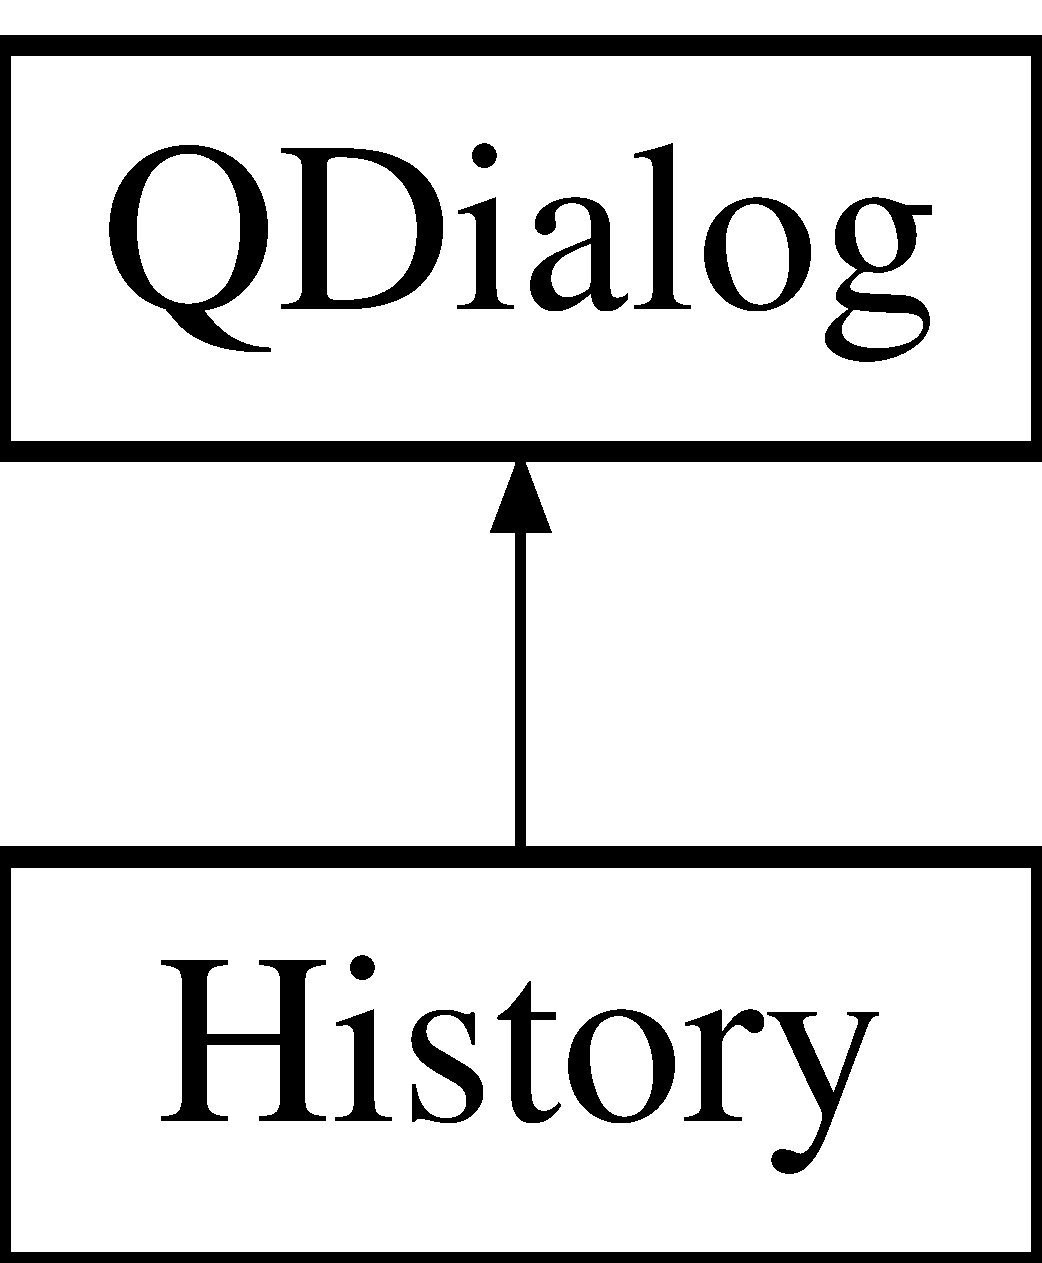
\includegraphics[height=2.000000cm]{classHistory}
\end{center}
\end{figure}
\subsection*{Public Member Functions}
\begin{DoxyCompactItemize}
\item 
\hyperlink{classHistory_af76054894d51c52a7e83fc33b5b879d3}{History} (Q\-Widget $\ast$parent=0, \hyperlink{classUser}{User} $\ast$user=new \hyperlink{classUser}{User}())
\item 
\hypertarget{classHistory_a5b00b64a1ddee04e60d5a3b517fd6d4c}{\hyperlink{classHistory_a5b00b64a1ddee04e60d5a3b517fd6d4c}{$\sim$\-History} ()}\label{classHistory_a5b00b64a1ddee04e60d5a3b517fd6d4c}

\begin{DoxyCompactList}\small\item\em destructor \end{DoxyCompactList}\end{DoxyCompactItemize}
\subsection*{Public Attributes}
\begin{DoxyCompactItemize}
\item 
\hypertarget{classHistory_afbec85a76b71689e5af9422b7be7e613}{\hyperlink{classUser}{User} $\ast$ {\bfseries user}}\label{classHistory_afbec85a76b71689e5af9422b7be7e613}

\end{DoxyCompactItemize}


\subsection{Constructor \& Destructor Documentation}
\hypertarget{classHistory_af76054894d51c52a7e83fc33b5b879d3}{\index{History@{History}!History@{History}}
\index{History@{History}!History@{History}}
\subsubsection[{History}]{\setlength{\rightskip}{0pt plus 5cm}History\-::\-History (
\begin{DoxyParamCaption}
\item[{Q\-Widget $\ast$}]{parent = {\ttfamily 0}, }
\item[{{\bf User} $\ast$}]{user = {\ttfamily new~{\bf User}()}}
\end{DoxyParamCaption}
)\hspace{0.3cm}{\ttfamily [explicit]}}}\label{classHistory_af76054894d51c52a7e83fc33b5b879d3}
$<$ displays highest score for the user for game1

$<$ displays highest score for the user for game2 

The documentation for this class was generated from the following files\-:\begin{DoxyCompactItemize}
\item 
history.\-h\item 
\hyperlink{history_8cpp}{history.\-cpp}\end{DoxyCompactItemize}

\hypertarget{classHome}{\section{Home Class Reference}
\label{classHome}\index{Home@{Home}}
}
Inheritance diagram for Home\-:\begin{figure}[H]
\begin{center}
\leavevmode
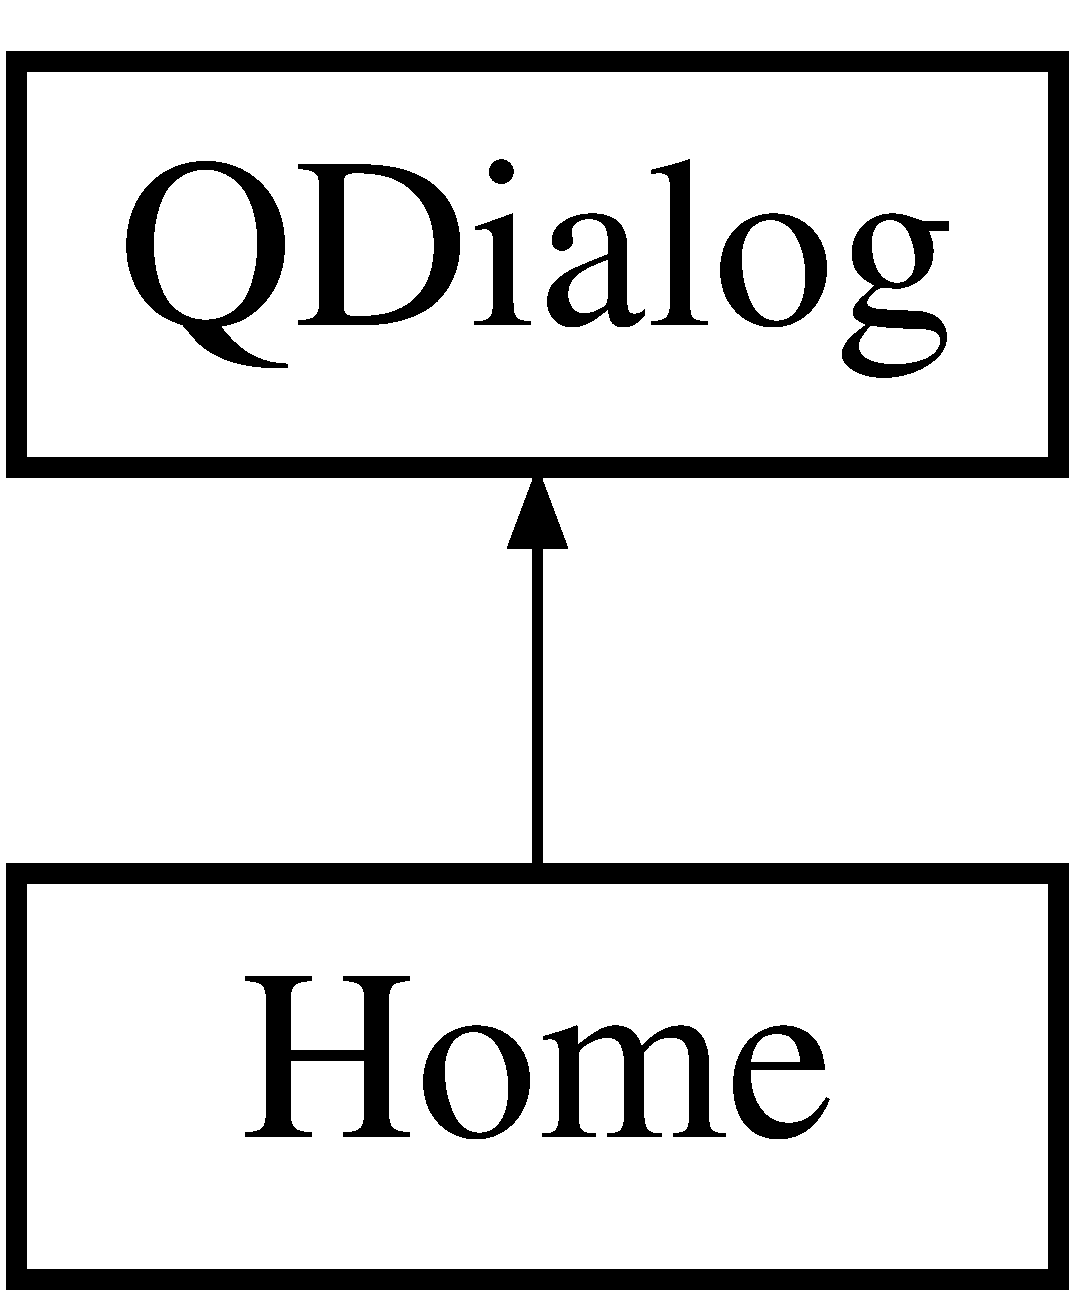
\includegraphics[height=2.000000cm]{classHome}
\end{center}
\end{figure}
\subsection*{Public Member Functions}
\begin{DoxyCompactItemize}
\item 
\hyperlink{classHome_a34931a02ab3581133828074a914c0e2f}{Home} (Q\-Widget $\ast$parent=0, \hyperlink{classUser}{User} $\ast$user=new \hyperlink{classUser}{User}())
\item 
\hypertarget{classHome_a7b27d4931b4b445d279202a098a0e8fd}{\hyperlink{classHome_a7b27d4931b4b445d279202a098a0e8fd}{$\sim$\-Home} ()}\label{classHome_a7b27d4931b4b445d279202a098a0e8fd}

\begin{DoxyCompactList}\small\item\em destructor \end{DoxyCompactList}\end{DoxyCompactItemize}
\subsection*{Public Attributes}
\begin{DoxyCompactItemize}
\item 
\hypertarget{classHome_a9fd10dbce3326f2b33321eb0bccb2e2e}{\hyperlink{classUser}{User} $\ast$ {\bfseries user}}\label{classHome_a9fd10dbce3326f2b33321eb0bccb2e2e}

\end{DoxyCompactItemize}


\subsection{Constructor \& Destructor Documentation}
\hypertarget{classHome_a34931a02ab3581133828074a914c0e2f}{\index{Home@{Home}!Home@{Home}}
\index{Home@{Home}!Home@{Home}}
\subsubsection[{Home}]{\setlength{\rightskip}{0pt plus 5cm}Home\-::\-Home (
\begin{DoxyParamCaption}
\item[{Q\-Widget $\ast$}]{parent = {\ttfamily 0}, }
\item[{{\bf User} $\ast$}]{user = {\ttfamily new~{\bf User}()}}
\end{DoxyParamCaption}
)\hspace{0.3cm}{\ttfamily [explicit]}}}\label{classHome_a34931a02ab3581133828074a914c0e2f}
$<$ happy birthday if his birthday is today 

The documentation for this class was generated from the following files\-:\begin{DoxyCompactItemize}
\item 
home.\-h\item 
\hyperlink{home_8cpp}{home.\-cpp}\end{DoxyCompactItemize}

\hypertarget{classHook}{\section{Hook Class Reference}
\label{classHook}\index{Hook@{Hook}}
}
Inheritance diagram for Hook\-:\begin{figure}[H]
\begin{center}
\leavevmode
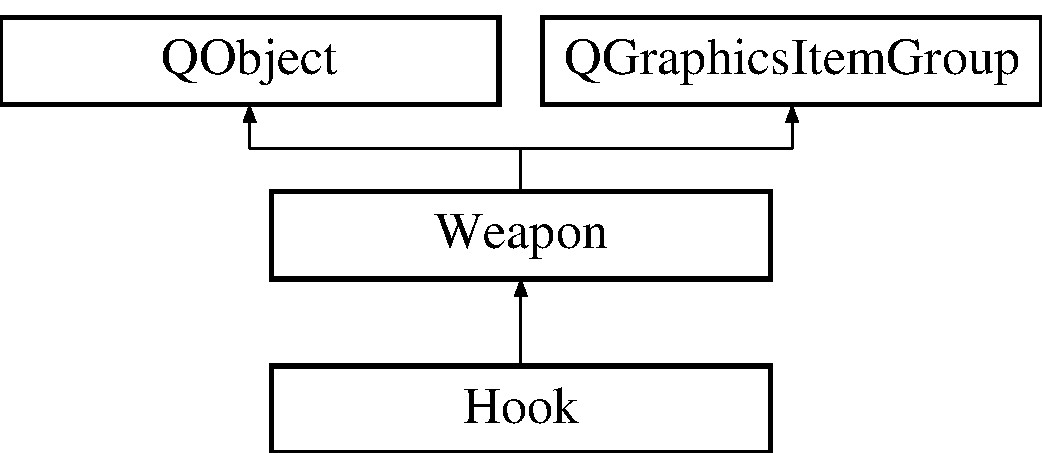
\includegraphics[height=3.000000cm]{classHook}
\end{center}
\end{figure}
\subsection*{Public Slots}
\begin{DoxyCompactItemize}
\item 
void \hyperlink{classHook_ac212ce64debced1f26243167bfcb750f}{update} ()
\begin{DoxyCompactList}\small\item\em \hyperlink{classHook_ac212ce64debced1f26243167bfcb750f}{Hook\-::update} the update function updates the length of the rope of the hook for a better graphical experience. \end{DoxyCompactList}\end{DoxyCompactItemize}
\subsection*{Public Member Functions}
\begin{DoxyCompactItemize}
\item 
\hyperlink{classHook_a144070c7b7fe467a7116de2734743257}{Hook} (int strength)
\begin{DoxyCompactList}\small\item\em \hyperlink{classHook_a144070c7b7fe467a7116de2734743257}{Hook\-::\-Hook}. \end{DoxyCompactList}\end{DoxyCompactItemize}
\subsection*{Additional Inherited Members}


\subsection{Constructor \& Destructor Documentation}
\hypertarget{classHook_a144070c7b7fe467a7116de2734743257}{\index{Hook@{Hook}!Hook@{Hook}}
\index{Hook@{Hook}!Hook@{Hook}}
\subsubsection[{Hook}]{\setlength{\rightskip}{0pt plus 5cm}Hook\-::\-Hook (
\begin{DoxyParamCaption}
\item[{int}]{strength}
\end{DoxyParamCaption}
)}}\label{classHook_a144070c7b7fe467a7116de2734743257}


\hyperlink{classHook_a144070c7b7fe467a7116de2734743257}{Hook\-::\-Hook}. 

constructor 
\begin{DoxyParams}{Parameters}
{\em strength} & used to specify the speed of movement of the hook. as the player gets stronger, the hook is faster \\
\hline
\end{DoxyParams}
initializing

drawing the rope

drawing the head of the hook

$<$ connecting the timer to an update function that updates the length of the hook 

\subsection{Member Function Documentation}
\hypertarget{classHook_ac212ce64debced1f26243167bfcb750f}{\index{Hook@{Hook}!update@{update}}
\index{update@{update}!Hook@{Hook}}
\subsubsection[{update}]{\setlength{\rightskip}{0pt plus 5cm}void Hook\-::update (
\begin{DoxyParamCaption}
{}
\end{DoxyParamCaption}
)\hspace{0.3cm}{\ttfamily [slot]}}}\label{classHook_ac212ce64debced1f26243167bfcb750f}


\hyperlink{classHook_ac212ce64debced1f26243167bfcb750f}{Hook\-::update} the update function updates the length of the rope of the hook for a better graphical experience. 

$<$ adding length to the rope

$<$ updating the position of the head

if the rope has reached its minimum length

if the rope has reached its maximum length

if it hasnt caught any item yet

checking for collisions

checking if the collision is with a grabbable item

updating attributes

in case it caught an item

$<$ positioning the item on the head of the hook 

The documentation for this class was generated from the following files\-:\begin{DoxyCompactItemize}
\item 
hook.\-h\item 
\hyperlink{hook_8cpp}{hook.\-cpp}\end{DoxyCompactItemize}

\hypertarget{classhuItem}{\section{hu\-Item Class Reference}
\label{classhuItem}\index{hu\-Item@{hu\-Item}}
}


\hyperlink{classhuItem}{hu\-Item} class  




{\ttfamily \#include $<$hu\-Item.\-h$>$}

Inheritance diagram for hu\-Item\-:\begin{figure}[H]
\begin{center}
\leavevmode
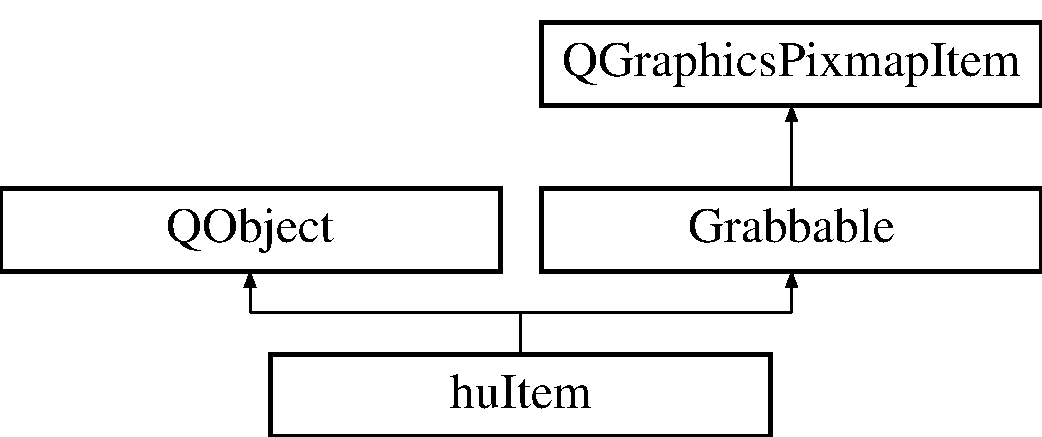
\includegraphics[height=3.000000cm]{classhuItem}
\end{center}
\end{figure}
\subsection*{Public Slots}
\begin{DoxyCompactItemize}
\item 
void \hyperlink{classhuItem_a3737ba343f040fed15febc7ef3e5ad52}{update} ()
\begin{DoxyCompactList}\small\item\em update the hu\-Itemss location on the screen \end{DoxyCompactList}\end{DoxyCompactItemize}
\subsection*{Public Member Functions}
\begin{DoxyCompactItemize}
\item 
\hypertarget{classhuItem_ab48bd1dc8b738ff323a8d72d4cbb4824}{{\bfseries hu\-Item} (bool type, \hyperlink{classHeader}{Header} $\ast$\hyperlink{classGrabbable_a97db8193dec83a8086352f80a30b2038}{header}, Q\-String game=\char`\"{}\char`\"{}, Q\-Object $\ast$parent=nullptr, int strength=0, int interval=100)}\label{classhuItem_ab48bd1dc8b738ff323a8d72d4cbb4824}

\item 
\hypertarget{classhuItem_a983ca578205dec2de2da458a9b055e5a}{\hyperlink{classhuItem_a983ca578205dec2de2da458a9b055e5a}{$\sim$hu\-Item} ()}\label{classhuItem_a983ca578205dec2de2da458a9b055e5a}

\begin{DoxyCompactList}\small\item\em destructor \end{DoxyCompactList}\end{DoxyCompactItemize}
\subsection*{Public Attributes}
\begin{DoxyCompactItemize}
\item 
\hypertarget{classhuItem_a69682e5b04939e293bd092613a6587dd}{Q\-Timer $\ast$ \hyperlink{classhuItem_a69682e5b04939e293bd092613a6587dd}{timer}}\label{classhuItem_a69682e5b04939e293bd092613a6587dd}

\begin{DoxyCompactList}\small\item\em timer attribute that specifies the timer \end{DoxyCompactList}\item 
\hypertarget{classhuItem_ae7fa9bc23a29a5efe04a6611ef787f65}{bool {\bfseries type}}\label{classhuItem_ae7fa9bc23a29a5efe04a6611ef787f65}

\item 
\hypertarget{classhuItem_a77a600419ccf8e6810b24ee4690e5331}{Q\-String {\bfseries game}}\label{classhuItem_a77a600419ccf8e6810b24ee4690e5331}

\end{DoxyCompactItemize}


\subsection{Detailed Description}
\hyperlink{classhuItem}{hu\-Item} class 

.h A hu\-Items is an element on screen that moves periodically in a predefined direction. 

\subsection{Member Function Documentation}
\hypertarget{classhuItem_a3737ba343f040fed15febc7ef3e5ad52}{\index{hu\-Item@{hu\-Item}!update@{update}}
\index{update@{update}!huItem@{hu\-Item}}
\subsubsection[{update}]{\setlength{\rightskip}{0pt plus 5cm}void hu\-Item\-::update (
\begin{DoxyParamCaption}
{}
\end{DoxyParamCaption}
)\hspace{0.3cm}{\ttfamily [slot]}}}\label{classhuItem_a3737ba343f040fed15febc7ef3e5ad52}


update the hu\-Itemss location on the screen 

\hyperlink{classhuItem_a3737ba343f040fed15febc7ef3e5ad52}{hu\-Item\-::update}

constantly updates the movement of the item in a downwards motion for game 1, and in an ellipse motion for game 2. for game 1\-: If the item collides with spongebob, his health is updated and the item is removed from the scene. If it collides with other items, it is not affected. additionally, when the item reaches the boundary of the scene, it is deleted.

for game 2\-: the item can be hooked or fired. if the item reaches the baby, based on its type, it might affect the babies health positivly or negatively. game 1

game 2

item is not grabbed yet

moves along a straigth downwards path first

then through an ellipse

then through a straight upwards path

removed from the scene if it has exceeded the defined path 

The documentation for this class was generated from the following files\-:\begin{DoxyCompactItemize}
\item 
hu\-Item.\-h\item 
\hyperlink{huItem_8cpp}{hu\-Item.\-cpp}\end{DoxyCompactItemize}

\hypertarget{classLaser}{\section{Laser Class Reference}
\label{classLaser}\index{Laser@{Laser}}
}
Inheritance diagram for Laser\-:\begin{figure}[H]
\begin{center}
\leavevmode
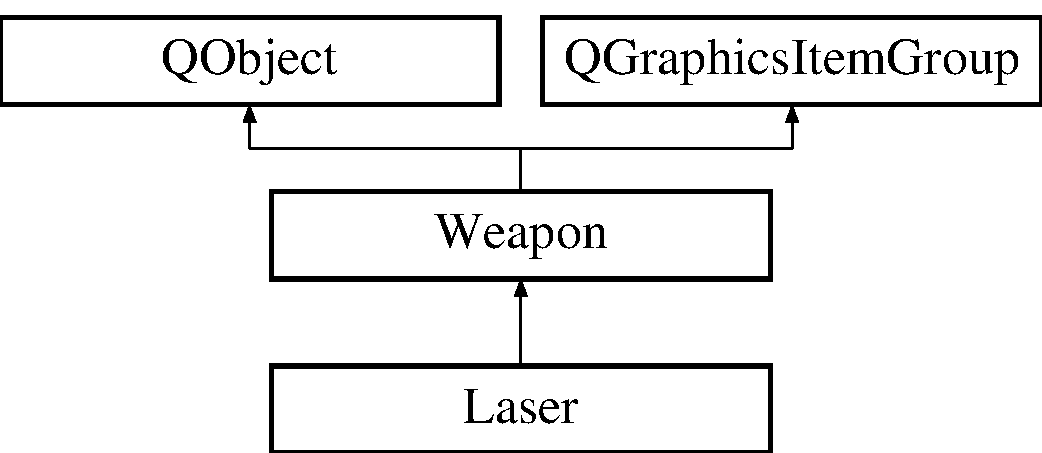
\includegraphics[height=3.000000cm]{classLaser}
\end{center}
\end{figure}
\subsection*{Public Slots}
\begin{DoxyCompactItemize}
\item 
void \hyperlink{classLaser_ae7317375cf2b7a5bff4281c359797255}{update} ()
\begin{DoxyCompactList}\small\item\em \hyperlink{classLaser_ae7317375cf2b7a5bff4281c359797255}{Laser\-::update} this function updates the length of the laser while shooting for a better user experience. It also checks for collisions and acts accordingly by calling other functions. \end{DoxyCompactList}\end{DoxyCompactItemize}
\subsection*{Public Member Functions}
\begin{DoxyCompactItemize}
\item 
\hypertarget{classLaser_a790db50423fe7ab34496b734210465c9}{\hyperlink{classLaser_a790db50423fe7ab34496b734210465c9}{Laser} (int strength)}\label{classLaser_a790db50423fe7ab34496b734210465c9}

\begin{DoxyCompactList}\small\item\em constructor \end{DoxyCompactList}\end{DoxyCompactItemize}
\subsection*{Additional Inherited Members}


\subsection{Member Function Documentation}
\hypertarget{classLaser_ae7317375cf2b7a5bff4281c359797255}{\index{Laser@{Laser}!update@{update}}
\index{update@{update}!Laser@{Laser}}
\subsubsection[{update}]{\setlength{\rightskip}{0pt plus 5cm}void Laser\-::update (
\begin{DoxyParamCaption}
{}
\end{DoxyParamCaption}
)\hspace{0.3cm}{\ttfamily [slot]}}}\label{classLaser_ae7317375cf2b7a5bff4281c359797255}


\hyperlink{classLaser_ae7317375cf2b7a5bff4281c359797255}{Laser\-::update} this function updates the length of the laser while shooting for a better user experience. It also checks for collisions and acts accordingly by calling other functions. 

check if there is a collison with a grabbable item (huitem)

$<$ stop elongating the laser

$<$ calling the wasshot function for updating metrics and removing the item from the scene 

The documentation for this class was generated from the following files\-:\begin{DoxyCompactItemize}
\item 
laser.\-h\item 
laser.\-cpp\end{DoxyCompactItemize}

\hypertarget{classPause}{\section{Pause Class Reference}
\label{classPause}\index{Pause@{Pause}}
}
Inheritance diagram for Pause\-:\begin{figure}[H]
\begin{center}
\leavevmode
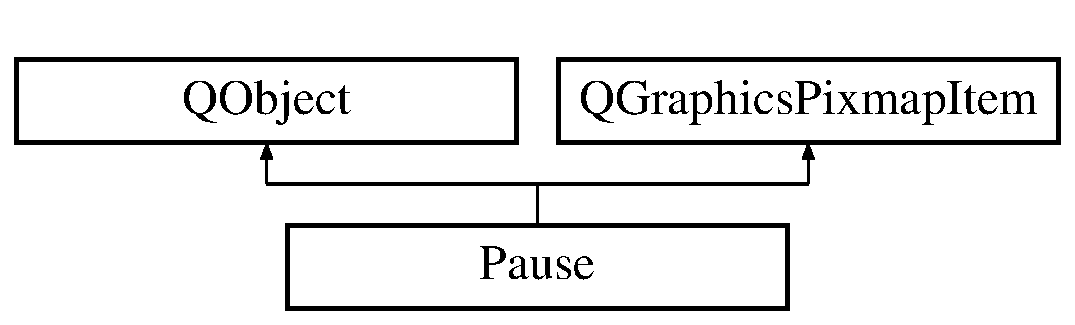
\includegraphics[height=2.000000cm]{classPause}
\end{center}
\end{figure}
\subsection*{Public Member Functions}
\begin{DoxyCompactItemize}
\item 
\hypertarget{classPause_a619b49e5a34f350da73a02605d982535}{{\bfseries Pause} (Q\-Object $\ast$parent=nullptr)}\label{classPause_a619b49e5a34f350da73a02605d982535}

\item 
\hypertarget{classPause_a1fe1549d3bc13a0868c1cf7458657760}{void {\bfseries mouse\-Release\-Event} (Q\-Graphics\-Scene\-Mouse\-Event $\ast$event)}\label{classPause_a1fe1549d3bc13a0868c1cf7458657760}

\end{DoxyCompactItemize}


The documentation for this class was generated from the following files\-:\begin{DoxyCompactItemize}
\item 
pause.\-h\item 
pause.\-cpp\end{DoxyCompactItemize}

\hypertarget{classScores}{\section{Scores Class Reference}
\label{classScores}\index{Scores@{Scores}}
}


The \hyperlink{classScores}{Scores} class.  




{\ttfamily \#include $<$scores.\-h$>$}

\subsection*{Static Public Member Functions}
\begin{DoxyCompactItemize}
\item 
static Q\-String \hyperlink{classScores_aa958c1c60267d4f682eb9e2580f94427}{Get\-Highest\-Score} (Q\-String game)
\begin{DoxyCompactList}\small\item\em \hyperlink{classScores_aa958c1c60267d4f682eb9e2580f94427}{Scores\-::\-Get\-Highest\-Score}. \end{DoxyCompactList}\item 
static Q\-String\-List \hyperlink{classScores_a73494bf10c0c62fada10f000086151f2}{Get\-User\-Scores} (Q\-String username, Q\-String game)
\begin{DoxyCompactList}\small\item\em \hyperlink{classScores_a73494bf10c0c62fada10f000086151f2}{Scores\-::\-Get\-User\-Scores}. \end{DoxyCompactList}\item 
static bool \hyperlink{classScores_a9b43bd9811f2582dbadb6021eaf6b193}{Add\-Score} (Q\-String username, Q\-String score, Q\-String game)
\begin{DoxyCompactList}\small\item\em \hyperlink{classScores_a9b43bd9811f2582dbadb6021eaf6b193}{Scores\-::\-Add\-Score}. \end{DoxyCompactList}\end{DoxyCompactItemize}


\subsection{Detailed Description}
The \hyperlink{classScores}{Scores} class. 

this class containes everything related to scores and manipulating them 

\subsection{Member Function Documentation}
\hypertarget{classScores_a9b43bd9811f2582dbadb6021eaf6b193}{\index{Scores@{Scores}!Add\-Score@{Add\-Score}}
\index{Add\-Score@{Add\-Score}!Scores@{Scores}}
\subsubsection[{Add\-Score}]{\setlength{\rightskip}{0pt plus 5cm}bool Scores\-::\-Add\-Score (
\begin{DoxyParamCaption}
\item[{Q\-String}]{username, }
\item[{Q\-String}]{score, }
\item[{Q\-String}]{game}
\end{DoxyParamCaption}
)\hspace{0.3cm}{\ttfamily [static]}}}\label{classScores_a9b43bd9811f2582dbadb6021eaf6b193}


\hyperlink{classScores_a9b43bd9811f2582dbadb6021eaf6b193}{Scores\-::\-Add\-Score}. 


\begin{DoxyParams}{Parameters}
{\em username} & \\
\hline
{\em score} & \\
\hline
{\em game} & \\
\hline
\end{DoxyParams}
\begin{DoxyReturn}{Returns}

\end{DoxyReturn}
this function adds a score to the list of scores for a selected user in a selected game \hypertarget{classScores_aa958c1c60267d4f682eb9e2580f94427}{\index{Scores@{Scores}!Get\-Highest\-Score@{Get\-Highest\-Score}}
\index{Get\-Highest\-Score@{Get\-Highest\-Score}!Scores@{Scores}}
\subsubsection[{Get\-Highest\-Score}]{\setlength{\rightskip}{0pt plus 5cm}Q\-String Scores\-::\-Get\-Highest\-Score (
\begin{DoxyParamCaption}
\item[{Q\-String}]{game}
\end{DoxyParamCaption}
)\hspace{0.3cm}{\ttfamily [static]}}}\label{classScores_aa958c1c60267d4f682eb9e2580f94427}


\hyperlink{classScores_aa958c1c60267d4f682eb9e2580f94427}{Scores\-::\-Get\-Highest\-Score}. 


\begin{DoxyParams}{Parameters}
{\em game} & \\
\hline
\end{DoxyParams}
\begin{DoxyReturn}{Returns}

\end{DoxyReturn}
this function gets the highest score in a given game from a Json Document \hypertarget{classScores_a73494bf10c0c62fada10f000086151f2}{\index{Scores@{Scores}!Get\-User\-Scores@{Get\-User\-Scores}}
\index{Get\-User\-Scores@{Get\-User\-Scores}!Scores@{Scores}}
\subsubsection[{Get\-User\-Scores}]{\setlength{\rightskip}{0pt plus 5cm}Q\-String\-List Scores\-::\-Get\-User\-Scores (
\begin{DoxyParamCaption}
\item[{Q\-String}]{username, }
\item[{Q\-String}]{game}
\end{DoxyParamCaption}
)\hspace{0.3cm}{\ttfamily [static]}}}\label{classScores_a73494bf10c0c62fada10f000086151f2}


\hyperlink{classScores_a73494bf10c0c62fada10f000086151f2}{Scores\-::\-Get\-User\-Scores}. 


\begin{DoxyParams}{Parameters}
{\em username} & \\
\hline
{\em game} & \\
\hline
\end{DoxyParams}
\begin{DoxyReturn}{Returns}

\end{DoxyReturn}
this function gets the scores of the user from a Json document 

The documentation for this class was generated from the following files\-:\begin{DoxyCompactItemize}
\item 
scores.\-h\item 
\hyperlink{scores_8cpp}{scores.\-cpp}\end{DoxyCompactItemize}

\hypertarget{classSignIn}{\section{Sign\-In Class Reference}
\label{classSignIn}\index{Sign\-In@{Sign\-In}}
}
Inheritance diagram for Sign\-In\-:\begin{figure}[H]
\begin{center}
\leavevmode
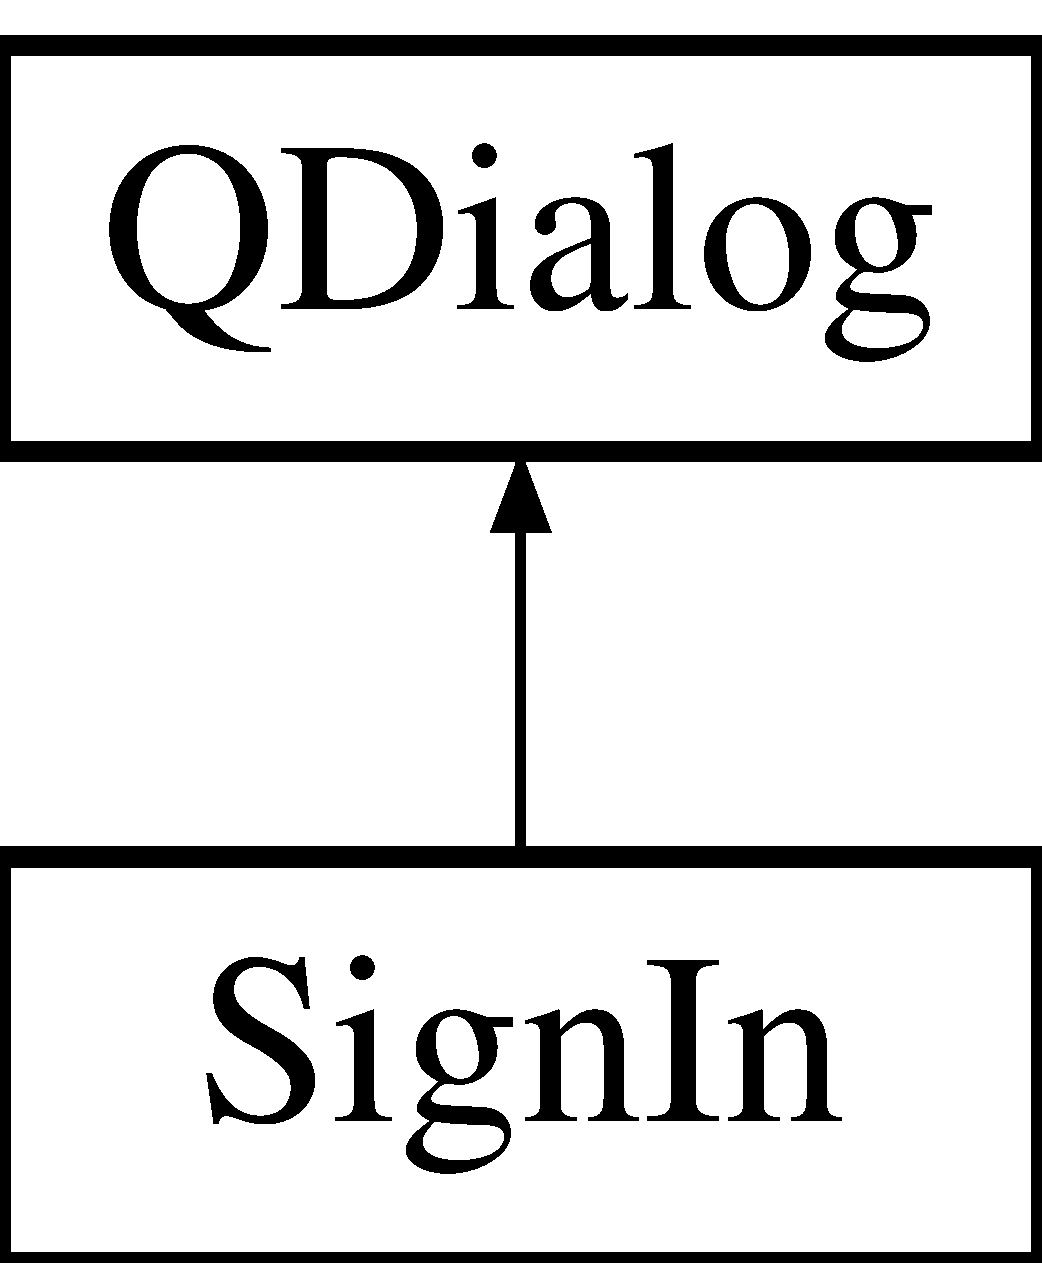
\includegraphics[height=2.000000cm]{classSignIn}
\end{center}
\end{figure}
\subsection*{Public Member Functions}
\begin{DoxyCompactItemize}
\item 
\hyperlink{classSignIn_a04e5dafeffb5598121044815b0059adc}{Sign\-In} (Q\-Widget $\ast$parent=0)
\begin{DoxyCompactList}\small\item\em \hyperlink{classSignIn_a04e5dafeffb5598121044815b0059adc}{Sign\-In\-::\-Sign\-In}. \end{DoxyCompactList}\item 
\hypertarget{classSignIn_a2595ba92e58b5f19935fcf4e00aa1432}{\hyperlink{classSignIn_a2595ba92e58b5f19935fcf4e00aa1432}{$\sim$\-Sign\-In} ()}\label{classSignIn_a2595ba92e58b5f19935fcf4e00aa1432}

\begin{DoxyCompactList}\small\item\em desctructor \end{DoxyCompactList}\end{DoxyCompactItemize}


\subsection{Constructor \& Destructor Documentation}
\hypertarget{classSignIn_a04e5dafeffb5598121044815b0059adc}{\index{Sign\-In@{Sign\-In}!Sign\-In@{Sign\-In}}
\index{Sign\-In@{Sign\-In}!SignIn@{Sign\-In}}
\subsubsection[{Sign\-In}]{\setlength{\rightskip}{0pt plus 5cm}Sign\-In\-::\-Sign\-In (
\begin{DoxyParamCaption}
\item[{Q\-Widget $\ast$}]{parent = {\ttfamily 0}}
\end{DoxyParamCaption}
)\hspace{0.3cm}{\ttfamily [explicit]}}}\label{classSignIn_a04e5dafeffb5598121044815b0059adc}


\hyperlink{classSignIn_a04e5dafeffb5598121044815b0059adc}{Sign\-In\-::\-Sign\-In}. 


\begin{DoxyParams}{Parameters}
{\em parent} & constructor \\
\hline
\end{DoxyParams}


The documentation for this class was generated from the following files\-:\begin{DoxyCompactItemize}
\item 
signin.\-h\item 
\hyperlink{signin_8cpp}{signin.\-cpp}\end{DoxyCompactItemize}

\hypertarget{classSignUp}{\section{Sign\-Up Class Reference}
\label{classSignUp}\index{Sign\-Up@{Sign\-Up}}
}
Inheritance diagram for Sign\-Up\-:\begin{figure}[H]
\begin{center}
\leavevmode
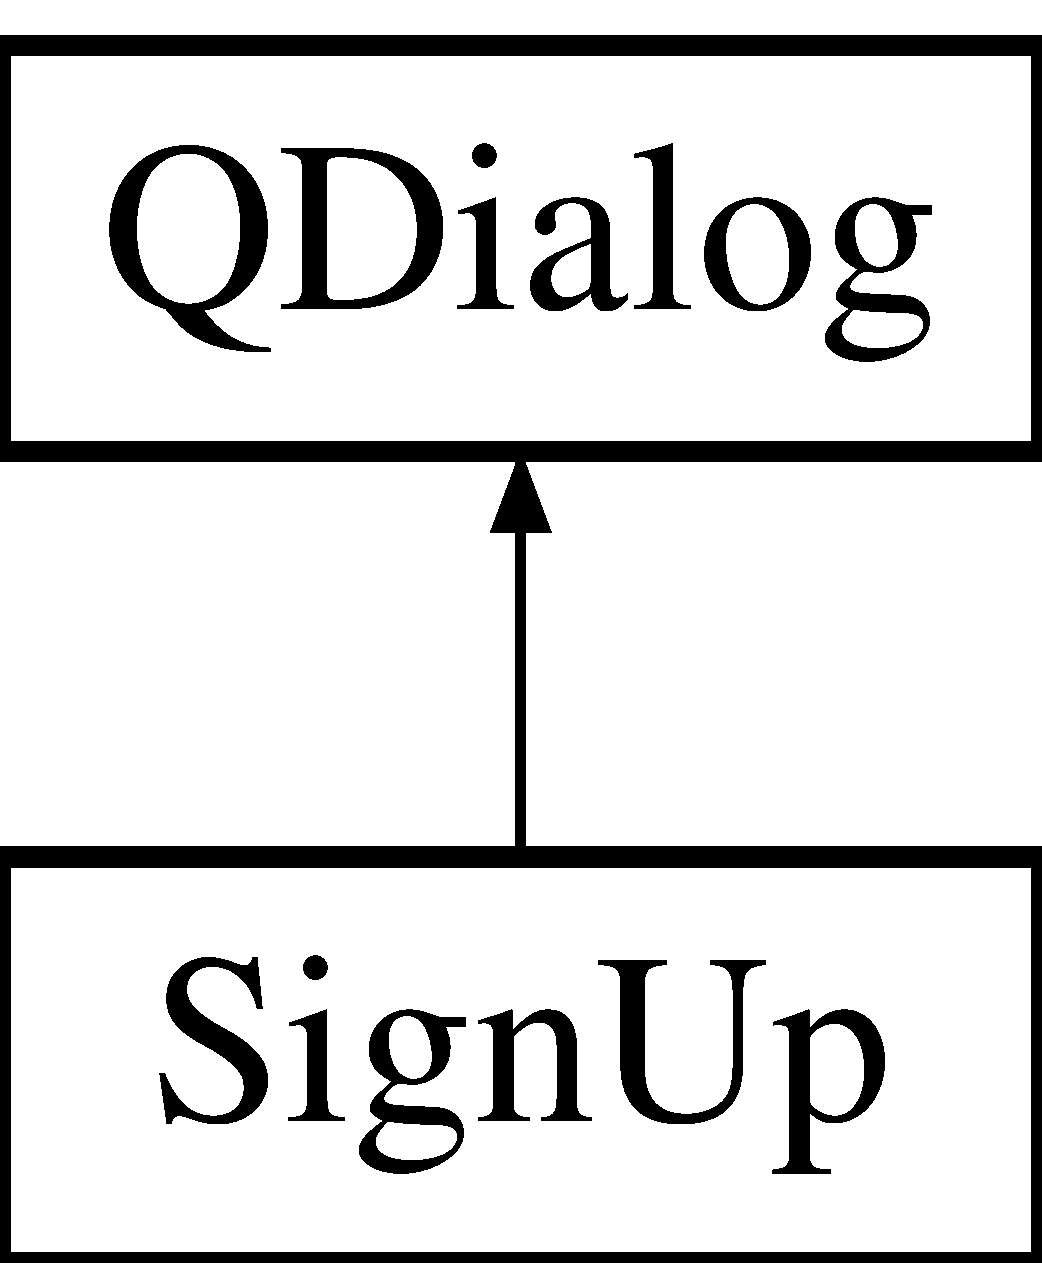
\includegraphics[height=2.000000cm]{classSignUp}
\end{center}
\end{figure}
\subsection*{Public Member Functions}
\begin{DoxyCompactItemize}
\item 
\hyperlink{classSignUp_a24c4f766e40f748e74f3c2d215c0c23c}{Sign\-Up} (Q\-Widget $\ast$parent=0)
\begin{DoxyCompactList}\small\item\em \hyperlink{classSignUp_a24c4f766e40f748e74f3c2d215c0c23c}{Sign\-Up\-::\-Sign\-Up}. \end{DoxyCompactList}\item 
\hypertarget{classSignUp_a361ad19f46cd8a70d0f661a841e3a63e}{\hyperlink{classSignUp_a361ad19f46cd8a70d0f661a841e3a63e}{$\sim$\-Sign\-Up} ()}\label{classSignUp_a361ad19f46cd8a70d0f661a841e3a63e}

\begin{DoxyCompactList}\small\item\em destructor \end{DoxyCompactList}\end{DoxyCompactItemize}
\subsection*{Public Attributes}
\begin{DoxyCompactItemize}
\item 
\hypertarget{classSignUp_a5f945a3243129bde03244b9861b1314c}{Q\-String {\bfseries profile\-Picture\-Edit}}\label{classSignUp_a5f945a3243129bde03244b9861b1314c}

\end{DoxyCompactItemize}


\subsection{Constructor \& Destructor Documentation}
\hypertarget{classSignUp_a24c4f766e40f748e74f3c2d215c0c23c}{\index{Sign\-Up@{Sign\-Up}!Sign\-Up@{Sign\-Up}}
\index{Sign\-Up@{Sign\-Up}!SignUp@{Sign\-Up}}
\subsubsection[{Sign\-Up}]{\setlength{\rightskip}{0pt plus 5cm}Sign\-Up\-::\-Sign\-Up (
\begin{DoxyParamCaption}
\item[{Q\-Widget $\ast$}]{parent = {\ttfamily 0}}
\end{DoxyParamCaption}
)\hspace{0.3cm}{\ttfamily [explicit]}}}\label{classSignUp_a24c4f766e40f748e74f3c2d215c0c23c}


\hyperlink{classSignUp_a24c4f766e40f748e74f3c2d215c0c23c}{Sign\-Up\-::\-Sign\-Up}. 


\begin{DoxyParams}{Parameters}
{\em parent} & constructor for the signup class. it hides the validation error messages \\
\hline
\end{DoxyParams}


The documentation for this class was generated from the following files\-:\begin{DoxyCompactItemize}
\item 
signup.\-h\item 
\hyperlink{signup_8cpp}{signup.\-cpp}\end{DoxyCompactItemize}

\hypertarget{classSpongeBob}{\section{Sponge\-Bob Class Reference}
\label{classSpongeBob}\index{Sponge\-Bob@{Sponge\-Bob}}
}


sponge\-Bob class  




{\ttfamily \#include $<$sponge\-Bob.\-h$>$}

Inheritance diagram for Sponge\-Bob\-:\begin{figure}[H]
\begin{center}
\leavevmode
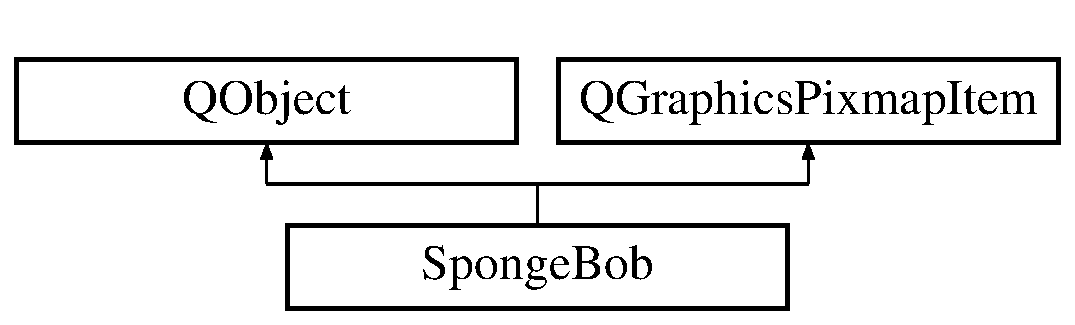
\includegraphics[height=2.000000cm]{classSpongeBob}
\end{center}
\end{figure}
\subsection*{Public Slots}
\begin{DoxyCompactItemize}
\item 
void \hyperlink{classSpongeBob_aabcc0812bd3801612c5328004748cc12}{toggle\-Follow} ()
\begin{DoxyCompactList}\small\item\em change from follow me to dont follow me \end{DoxyCompactList}\end{DoxyCompactItemize}
\subsection*{Public Member Functions}
\begin{DoxyCompactItemize}
\item 
\hyperlink{classSpongeBob_acd6c5412c662a93f4f91d8888cfef804}{Sponge\-Bob} (int \hyperlink{classSpongeBob_a09c3ee16b44a4a89a014f6055868a9e5}{cleanliness}, int \hyperlink{classSpongeBob_a72a16aa8925690a274e869c0eb0a9fd5}{immunity}, int \hyperlink{classSpongeBob_a801b813e51511cb779f077e6b510eb56}{lives}, int \hyperlink{classSpongeBob_a24b14e1237cb158488cb1bcf84b42d13}{score}, Q\-Point pos, Q\-String \hyperlink{classSpongeBob_a271879173f8458be51a074e89e694403}{game}, Q\-Object $\ast$parent=nullptr, int bombs=0, int required\-Bomb\-Score=0, int translation=0, Q\-String \hyperlink{classSpongeBob_a264d204946dc5aea60f5f2126fc546d3}{weapon}=\char`\"{}\char`\"{}, int weapon\-Strength=0)
\begin{DoxyCompactList}\small\item\em constructor \end{DoxyCompactList}\item 
void \hyperlink{classSpongeBob_a489d205da14cfc2760cba9624eb03772}{key\-Press\-Event} (Q\-Key\-Event $\ast$event)
\begin{DoxyCompactList}\small\item\em Detects key strokes pressed. \end{DoxyCompactList}\item 
void \hyperlink{classSpongeBob_a8e01b8481b4b5af4072ab6973cbf761f}{key\-Release\-Event} (Q\-Key\-Event $\ast$event)
\begin{DoxyCompactList}\small\item\em Detects key release events. \end{DoxyCompactList}\end{DoxyCompactItemize}
\subsection*{Public Attributes}
\begin{DoxyCompactItemize}
\item 
\hypertarget{classSpongeBob_a124a05c347340041b19c187b0e11d28e}{bool \hyperlink{classSpongeBob_a124a05c347340041b19c187b0e11d28e}{followme}}\label{classSpongeBob_a124a05c347340041b19c187b0e11d28e}

\begin{DoxyCompactList}\small\item\em followme attribute that specifies if the bacteria should follow spongebob or not \end{DoxyCompactList}\item 
\hypertarget{classSpongeBob_aaa7f8e848ec158ce5d03e3a782026d6d}{Q\-Timer $\ast$ \hyperlink{classSpongeBob_aaa7f8e848ec158ce5d03e3a782026d6d}{follow\-Timer}}\label{classSpongeBob_aaa7f8e848ec158ce5d03e3a782026d6d}

\begin{DoxyCompactList}\small\item\em timer attribute that specifies the timer \end{DoxyCompactList}\item 
\hypertarget{classSpongeBob_a09c3ee16b44a4a89a014f6055868a9e5}{int \hyperlink{classSpongeBob_a09c3ee16b44a4a89a014f6055868a9e5}{cleanliness}}\label{classSpongeBob_a09c3ee16b44a4a89a014f6055868a9e5}

\begin{DoxyCompactList}\small\item\em cleanliness of the tank \end{DoxyCompactList}\item 
\hypertarget{classSpongeBob_a72a16aa8925690a274e869c0eb0a9fd5}{int \hyperlink{classSpongeBob_a72a16aa8925690a274e869c0eb0a9fd5}{immunity}}\label{classSpongeBob_a72a16aa8925690a274e869c0eb0a9fd5}

\begin{DoxyCompactList}\small\item\em immunity level of spongebob \end{DoxyCompactList}\item 
\hypertarget{classSpongeBob_a801b813e51511cb779f077e6b510eb56}{int \hyperlink{classSpongeBob_a801b813e51511cb779f077e6b510eb56}{lives}}\label{classSpongeBob_a801b813e51511cb779f077e6b510eb56}

\begin{DoxyCompactList}\small\item\em number of lives \end{DoxyCompactList}\item 
\hypertarget{classSpongeBob_a24b14e1237cb158488cb1bcf84b42d13}{int \hyperlink{classSpongeBob_a24b14e1237cb158488cb1bcf84b42d13}{score}}\label{classSpongeBob_a24b14e1237cb158488cb1bcf84b42d13}

\begin{DoxyCompactList}\small\item\em total score \end{DoxyCompactList}\item 
\hypertarget{classSpongeBob_aaa6688a6fcf12b0eae3fd3a7f1e137bc}{Q\-Point \hyperlink{classSpongeBob_aaa6688a6fcf12b0eae3fd3a7f1e137bc}{current\-Pos}}\label{classSpongeBob_aaa6688a6fcf12b0eae3fd3a7f1e137bc}

\begin{DoxyCompactList}\small\item\em current position \end{DoxyCompactList}\item 
\hypertarget{classSpongeBob_a264d204946dc5aea60f5f2126fc546d3}{\hyperlink{classWeapon}{Weapon} $\ast$ \hyperlink{classSpongeBob_a264d204946dc5aea60f5f2126fc546d3}{weapon}}\label{classSpongeBob_a264d204946dc5aea60f5f2126fc546d3}

\begin{DoxyCompactList}\small\item\em pointer to the weapon used \end{DoxyCompactList}\item 
\hypertarget{classSpongeBob_a271879173f8458be51a074e89e694403}{Q\-String \hyperlink{classSpongeBob_a271879173f8458be51a074e89e694403}{game}}\label{classSpongeBob_a271879173f8458be51a074e89e694403}

\begin{DoxyCompactList}\small\item\em specify the game to which the instance belongs ( game1 or game2) \end{DoxyCompactList}\item 
\hypertarget{classSpongeBob_a771d252ba5afccc3c428a39e200453fe}{int {\bfseries translation}}\label{classSpongeBob_a771d252ba5afccc3c428a39e200453fe}

\item 
\hypertarget{classSpongeBob_ad9376b9f927ada8f5e9c9871bd86c7ff}{int {\bfseries bombs}}\label{classSpongeBob_ad9376b9f927ada8f5e9c9871bd86c7ff}

\item 
\hypertarget{classSpongeBob_a7dc982197904d3a4f04f8e5d88da80ef}{int {\bfseries required\-Bomb\-Score}}\label{classSpongeBob_a7dc982197904d3a4f04f8e5d88da80ef}

\end{DoxyCompactItemize}


\subsection{Detailed Description}
sponge\-Bob class 

.h This creates an instance of the spongebob. 

\subsection{Constructor \& Destructor Documentation}
\hypertarget{classSpongeBob_acd6c5412c662a93f4f91d8888cfef804}{\index{Sponge\-Bob@{Sponge\-Bob}!Sponge\-Bob@{Sponge\-Bob}}
\index{Sponge\-Bob@{Sponge\-Bob}!SpongeBob@{Sponge\-Bob}}
\subsubsection[{Sponge\-Bob}]{\setlength{\rightskip}{0pt plus 5cm}Sponge\-Bob\-::\-Sponge\-Bob (
\begin{DoxyParamCaption}
\item[{int}]{cleanliness, }
\item[{int}]{immunity, }
\item[{int}]{lives, }
\item[{int}]{score, }
\item[{Q\-Point}]{pos, }
\item[{Q\-String}]{game, }
\item[{Q\-Object $\ast$}]{parent = {\ttfamily nullptr}, }
\item[{int}]{bombs = {\ttfamily 0}, }
\item[{int}]{required\-Bomb\-Score = {\ttfamily 0}, }
\item[{int}]{translation = {\ttfamily 0}, }
\item[{Q\-String}]{weapon = {\ttfamily \char`\"{}\char`\"{}}, }
\item[{int}]{weapon\-Strength = {\ttfamily 0}}
\end{DoxyParamCaption}
)\hspace{0.3cm}{\ttfamily [explicit]}}}\label{classSpongeBob_acd6c5412c662a93f4f91d8888cfef804}


constructor 

setting up attributes of spongebob 

\subsection{Member Function Documentation}
\hypertarget{classSpongeBob_a489d205da14cfc2760cba9624eb03772}{\index{Sponge\-Bob@{Sponge\-Bob}!key\-Press\-Event@{key\-Press\-Event}}
\index{key\-Press\-Event@{key\-Press\-Event}!SpongeBob@{Sponge\-Bob}}
\subsubsection[{key\-Press\-Event}]{\setlength{\rightskip}{0pt plus 5cm}void Sponge\-Bob\-::key\-Press\-Event (
\begin{DoxyParamCaption}
\item[{Q\-Key\-Event $\ast$}]{event}
\end{DoxyParamCaption}
)}}\label{classSpongeBob_a489d205da14cfc2760cba9624eb03772}


Detects key strokes pressed. 

sponge\-Bob\-::key\-Press\-Event


\begin{DoxyParams}{Parameters}
{\em $\ast$event} & first argument, keystroke event\\
\hline
{\em event} & the keypress event detects all key strokes on the keyboard. we are only interested in the up,down,left, and right strokes when one of those keys is pressed, spongebob moves accoringly when possible. it also moves diagonally if multiple of these keys are pressed at the same time. Sponge bob moves diagonally faster than horizontally and vertically if the location of spongebob is on the edges of the screen, the position isnt updated if this will result in leaving the screen \\
\hline
\end{DoxyParams}
game 1 movement

the x key fires the weapon

the z key changes the weapon

if the player has the required score and has bombs \hypertarget{classSpongeBob_a8e01b8481b4b5af4072ab6973cbf761f}{\index{Sponge\-Bob@{Sponge\-Bob}!key\-Release\-Event@{key\-Release\-Event}}
\index{key\-Release\-Event@{key\-Release\-Event}!SpongeBob@{Sponge\-Bob}}
\subsubsection[{key\-Release\-Event}]{\setlength{\rightskip}{0pt plus 5cm}void Sponge\-Bob\-::key\-Release\-Event (
\begin{DoxyParamCaption}
\item[{Q\-Key\-Event $\ast$}]{event}
\end{DoxyParamCaption}
)}}\label{classSpongeBob_a8e01b8481b4b5af4072ab6973cbf761f}


Detects key release events. 

sponge\-Bob\-::key\-Release\-Event


\begin{DoxyParams}{Parameters}
{\em $\ast$event} & first argument, key release event\\
\hline
{\em event} & this collects key release events and removes them from the set of pressed keys \\
\hline
\end{DoxyParams}
\hypertarget{classSpongeBob_aabcc0812bd3801612c5328004748cc12}{\index{Sponge\-Bob@{Sponge\-Bob}!toggle\-Follow@{toggle\-Follow}}
\index{toggle\-Follow@{toggle\-Follow}!SpongeBob@{Sponge\-Bob}}
\subsubsection[{toggle\-Follow}]{\setlength{\rightskip}{0pt plus 5cm}void Sponge\-Bob\-::toggle\-Follow (
\begin{DoxyParamCaption}
{}
\end{DoxyParamCaption}
)\hspace{0.3cm}{\ttfamily [slot]}}}\label{classSpongeBob_aabcc0812bd3801612c5328004748cc12}


change from follow me to dont follow me 

sponge\-Bob\-::toggle\-Follow toggles the follow me to false when the timer ends 

The documentation for this class was generated from the following files\-:\begin{DoxyCompactItemize}
\item 
sponge\-Bob.\-h\item 
\hyperlink{spongeBob_8cpp}{sponge\-Bob.\-cpp}\end{DoxyCompactItemize}

\hypertarget{classUser}{\section{User Class Reference}
\label{classUser}\index{User@{User}}
}
\subsection*{Public Member Functions}
\begin{DoxyCompactItemize}
\item 
\hyperlink{classUser_a49af102252f983aa3d85bd59193c9bf1}{User} (Q\-String username, Q\-String password, Q\-String first\-Name, Q\-String last\-Name, Q\-String date\-Of\-Birth, Q\-String gender, Q\-Image profile\-Picture)
\end{DoxyCompactItemize}
\subsection*{Static Public Member Functions}
\begin{DoxyCompactItemize}
\item 
static bool \hyperlink{classUser_aa80c06d9b3076301a3b36831ad8324dc}{Add\-User} (\hyperlink{classUser}{User} user)
\begin{DoxyCompactList}\small\item\em \hyperlink{classUser_aa80c06d9b3076301a3b36831ad8324dc}{User\-::\-Add\-User}. \end{DoxyCompactList}\item 
static \hyperlink{classUser}{User} $\ast$ \hyperlink{classUser_a79a561251d56226e81062affe8312a09}{Get\-User} (Q\-String username, Q\-String password)
\begin{DoxyCompactList}\small\item\em \hyperlink{classUser_a79a561251d56226e81062affe8312a09}{User\-::\-Get\-User}. \end{DoxyCompactList}\item 
static Q\-Json\-Object \hyperlink{classUser_aa4ecad468e06bde01b44b4b2fd1186a6}{User\-To\-Json} (\hyperlink{classUser}{User} user)
\begin{DoxyCompactList}\small\item\em \hyperlink{classUser_aa4ecad468e06bde01b44b4b2fd1186a6}{User\-::\-User\-To\-Json}. \end{DoxyCompactList}\item 
static \hyperlink{classUser}{User} $\ast$ \hyperlink{classUser_a672d3246cd8890263bc359af137e0f41}{Json\-To\-User} (Q\-Json\-Object object, Q\-String username)
\begin{DoxyCompactList}\small\item\em \hyperlink{classUser_a672d3246cd8890263bc359af137e0f41}{User\-::\-Json\-To\-User}. \end{DoxyCompactList}\item 
static void \hyperlink{classUser_af72d21ca380b5ec3697978a1cbd8bec1}{Pause\-Game\-For\-User} (\hyperlink{classHeader}{Header} $\ast$header, bool completed)
\item 
static \hyperlink{classHeader}{Header} $\ast$ \hyperlink{classUser_afc56ee5edbdbdb8c95d6d869e95c23f5}{Resume\-Game\-For\-User} (Q\-String game, Q\-String username)
\item 
\hypertarget{classUser_a2166948eb636ad50a7e613e422e08ad8}{static int \hyperlink{classUser_a2166948eb636ad50a7e613e422e08ad8}{Get\-User\-Level} (Q\-String game, Q\-String username)}\label{classUser_a2166948eb636ad50a7e613e422e08ad8}

\begin{DoxyCompactList}\small\item\em this function is used to get the current level of the user in a specific game \end{DoxyCompactList}\item 
static void \hyperlink{classUser_a90499a55331bf2e55ff274e0ffa143fe}{Upgrade\-User\-To\-Level} (Q\-String game, Q\-String username, int level)
\begin{DoxyCompactList}\small\item\em \hyperlink{classUser_a90499a55331bf2e55ff274e0ffa143fe}{User\-::\-Upgrade\-User\-To\-Level}. \end{DoxyCompactList}\end{DoxyCompactItemize}
\subsection*{Public Attributes}
\begin{DoxyCompactItemize}
\item 
\hypertarget{classUser_a926d834a6d4c7c46e1dc1783bb7a1447}{Q\-String {\bfseries Username}}\label{classUser_a926d834a6d4c7c46e1dc1783bb7a1447}

\item 
\hypertarget{classUser_a25dc93a925a47f6bd3231002618d057d}{Q\-String {\bfseries Password}}\label{classUser_a25dc93a925a47f6bd3231002618d057d}

\item 
\hypertarget{classUser_a1af9ae238c93f4f0cde6c5fde7d2976f}{Q\-String {\bfseries First\-Name}}\label{classUser_a1af9ae238c93f4f0cde6c5fde7d2976f}

\item 
\hypertarget{classUser_ad57254a70a3ec42742ffc323bcce27d6}{Q\-String {\bfseries Last\-Name}}\label{classUser_ad57254a70a3ec42742ffc323bcce27d6}

\item 
\hypertarget{classUser_a9cb4f9257b748f960a8c6a6b3426ff97}{Q\-String {\bfseries Date\-Of\-Birth}}\label{classUser_a9cb4f9257b748f960a8c6a6b3426ff97}

\item 
\hypertarget{classUser_ad946499bcf2074d130071b8f18b528de}{Q\-String {\bfseries Gender}}\label{classUser_ad946499bcf2074d130071b8f18b528de}

\item 
\hypertarget{classUser_a65e02853585b9fb2819fe11f67aefa1e}{Q\-Image {\bfseries Profile\-Picture}}\label{classUser_a65e02853585b9fb2819fe11f67aefa1e}

\end{DoxyCompactItemize}


\subsection{Constructor \& Destructor Documentation}
\hypertarget{classUser_a49af102252f983aa3d85bd59193c9bf1}{\index{User@{User}!User@{User}}
\index{User@{User}!User@{User}}
\subsubsection[{User}]{\setlength{\rightskip}{0pt plus 5cm}User\-::\-User (
\begin{DoxyParamCaption}
\item[{Q\-String}]{username, }
\item[{Q\-String}]{password, }
\item[{Q\-String}]{first\-Name, }
\item[{Q\-String}]{last\-Name, }
\item[{Q\-String}]{date\-Of\-Birth, }
\item[{Q\-String}]{gender, }
\item[{Q\-Image}]{profile\-Picture}
\end{DoxyParamCaption}
)\hspace{0.3cm}{\ttfamily [explicit]}}}\label{classUser_a49af102252f983aa3d85bd59193c9bf1}
setting attributes 

\subsection{Member Function Documentation}
\hypertarget{classUser_aa80c06d9b3076301a3b36831ad8324dc}{\index{User@{User}!Add\-User@{Add\-User}}
\index{Add\-User@{Add\-User}!User@{User}}
\subsubsection[{Add\-User}]{\setlength{\rightskip}{0pt plus 5cm}bool User\-::\-Add\-User (
\begin{DoxyParamCaption}
\item[{{\bf User}}]{user}
\end{DoxyParamCaption}
)\hspace{0.3cm}{\ttfamily [static]}}}\label{classUser_aa80c06d9b3076301a3b36831ad8324dc}


\hyperlink{classUser_aa80c06d9b3076301a3b36831ad8324dc}{User\-::\-Add\-User}. 


\begin{DoxyParams}{Parameters}
{\em user} & \\
\hline
\end{DoxyParams}
\begin{DoxyReturn}{Returns}

\end{DoxyReturn}
this function adds a new user and saves the records to the json file \hypertarget{classUser_a79a561251d56226e81062affe8312a09}{\index{User@{User}!Get\-User@{Get\-User}}
\index{Get\-User@{Get\-User}!User@{User}}
\subsubsection[{Get\-User}]{\setlength{\rightskip}{0pt plus 5cm}{\bf User} $\ast$ User\-::\-Get\-User (
\begin{DoxyParamCaption}
\item[{Q\-String}]{username, }
\item[{Q\-String}]{password}
\end{DoxyParamCaption}
)\hspace{0.3cm}{\ttfamily [static]}}}\label{classUser_a79a561251d56226e81062affe8312a09}


\hyperlink{classUser_a79a561251d56226e81062affe8312a09}{User\-::\-Get\-User}. 


\begin{DoxyParams}{Parameters}
{\em username} & \\
\hline
{\em password} & \\
\hline
\end{DoxyParams}
\begin{DoxyReturn}{Returns}

\end{DoxyReturn}
this function searches for a user based on a username and a password \hypertarget{classUser_a672d3246cd8890263bc359af137e0f41}{\index{User@{User}!Json\-To\-User@{Json\-To\-User}}
\index{Json\-To\-User@{Json\-To\-User}!User@{User}}
\subsubsection[{Json\-To\-User}]{\setlength{\rightskip}{0pt plus 5cm}{\bf User} $\ast$ User\-::\-Json\-To\-User (
\begin{DoxyParamCaption}
\item[{Q\-Json\-Object}]{object, }
\item[{Q\-String}]{username}
\end{DoxyParamCaption}
)\hspace{0.3cm}{\ttfamily [static]}}}\label{classUser_a672d3246cd8890263bc359af137e0f41}


\hyperlink{classUser_a672d3246cd8890263bc359af137e0f41}{User\-::\-Json\-To\-User}. 


\begin{DoxyParams}{Parameters}
{\em object} & \\
\hline
{\em username} & \\
\hline
\end{DoxyParams}
\begin{DoxyReturn}{Returns}

\end{DoxyReturn}
this function takes a json object and parses it to an user object \hypertarget{classUser_af72d21ca380b5ec3697978a1cbd8bec1}{\index{User@{User}!Pause\-Game\-For\-User@{Pause\-Game\-For\-User}}
\index{Pause\-Game\-For\-User@{Pause\-Game\-For\-User}!User@{User}}
\subsubsection[{Pause\-Game\-For\-User}]{\setlength{\rightskip}{0pt plus 5cm}void User\-::\-Pause\-Game\-For\-User (
\begin{DoxyParamCaption}
\item[{{\bf Header} $\ast$}]{header, }
\item[{bool}]{completed}
\end{DoxyParamCaption}
)\hspace{0.3cm}{\ttfamily [static]}}}\label{classUser_af72d21ca380b5ec3697978a1cbd8bec1}
this function is used to pause the game for later access. it saves the data in a json document. the values of attributes in the header are saved. \hypertarget{classUser_afc56ee5edbdbdb8c95d6d869e95c23f5}{\index{User@{User}!Resume\-Game\-For\-User@{Resume\-Game\-For\-User}}
\index{Resume\-Game\-For\-User@{Resume\-Game\-For\-User}!User@{User}}
\subsubsection[{Resume\-Game\-For\-User}]{\setlength{\rightskip}{0pt plus 5cm}{\bf Header} $\ast$ User\-::\-Resume\-Game\-For\-User (
\begin{DoxyParamCaption}
\item[{Q\-String}]{game, }
\item[{Q\-String}]{username}
\end{DoxyParamCaption}
)\hspace{0.3cm}{\ttfamily [static]}}}\label{classUser_afc56ee5edbdbdb8c95d6d869e95c23f5}
this function is given a game and a username, and is used to check if there are available paused games for the user. if there is a paused game, an instance of header and spongebob are created and filled with the previously saved state. initializing according to previous metrics

initializing according to previous metrics

initializing according to previous metrics

initializing according to previous metrics \hypertarget{classUser_a90499a55331bf2e55ff274e0ffa143fe}{\index{User@{User}!Upgrade\-User\-To\-Level@{Upgrade\-User\-To\-Level}}
\index{Upgrade\-User\-To\-Level@{Upgrade\-User\-To\-Level}!User@{User}}
\subsubsection[{Upgrade\-User\-To\-Level}]{\setlength{\rightskip}{0pt plus 5cm}void User\-::\-Upgrade\-User\-To\-Level (
\begin{DoxyParamCaption}
\item[{Q\-String}]{game, }
\item[{Q\-String}]{username, }
\item[{int}]{level}
\end{DoxyParamCaption}
)\hspace{0.3cm}{\ttfamily [static]}}}\label{classUser_a90499a55331bf2e55ff274e0ffa143fe}


\hyperlink{classUser_a90499a55331bf2e55ff274e0ffa143fe}{User\-::\-Upgrade\-User\-To\-Level}. 


\begin{DoxyParams}{Parameters}
{\em game} & \\
\hline
{\em username} & \\
\hline
{\em level} & this function is called whith a game, a username, and a level. it gets the json object of the user using its username, and then assigns him a higher level on the given game. this allows the user to play the game on a higher level. \\
\hline
\end{DoxyParams}
\hypertarget{classUser_aa4ecad468e06bde01b44b4b2fd1186a6}{\index{User@{User}!User\-To\-Json@{User\-To\-Json}}
\index{User\-To\-Json@{User\-To\-Json}!User@{User}}
\subsubsection[{User\-To\-Json}]{\setlength{\rightskip}{0pt plus 5cm}Q\-Json\-Object User\-::\-User\-To\-Json (
\begin{DoxyParamCaption}
\item[{{\bf User}}]{user}
\end{DoxyParamCaption}
)\hspace{0.3cm}{\ttfamily [static]}}}\label{classUser_aa4ecad468e06bde01b44b4b2fd1186a6}


\hyperlink{classUser_aa4ecad468e06bde01b44b4b2fd1186a6}{User\-::\-User\-To\-Json}. 


\begin{DoxyParams}{Parameters}
{\em user} & \\
\hline
\end{DoxyParams}
\begin{DoxyReturn}{Returns}

\end{DoxyReturn}
this function takes an instance of a user and converts its attributes to a json object 

The documentation for this class was generated from the following files\-:\begin{DoxyCompactItemize}
\item 
user.\-h\item 
user.\-cpp\end{DoxyCompactItemize}

\hypertarget{classvirus}{\section{virus Class Reference}
\label{classvirus}\index{virus@{virus}}
}


virus class  




{\ttfamily \#include $<$virus.\-h$>$}

Inheritance diagram for virus\-:\begin{figure}[H]
\begin{center}
\leavevmode
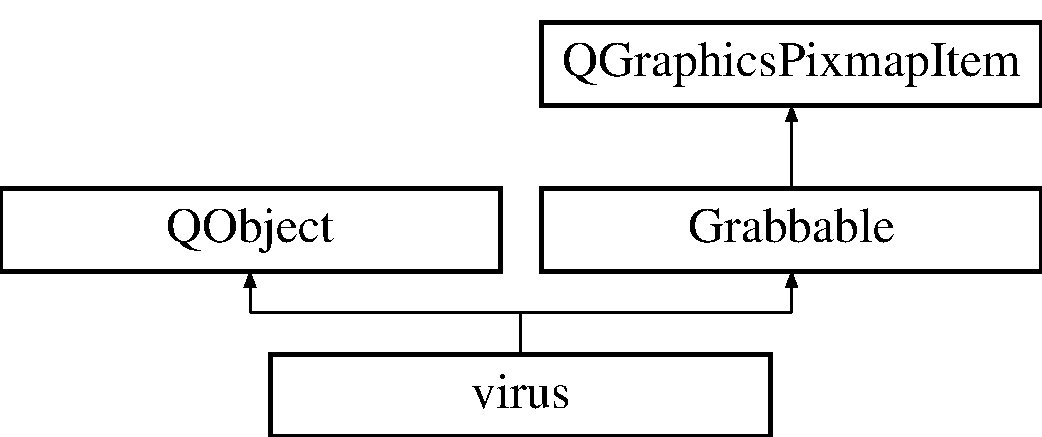
\includegraphics[height=3.000000cm]{classvirus}
\end{center}
\end{figure}
\subsection*{Public Slots}
\begin{DoxyCompactItemize}
\item 
void \hyperlink{classvirus_a8b036fc788433ad3a705e9de6de41ee2}{update} ()
\begin{DoxyCompactList}\small\item\em update the location on the screen and detects collision \end{DoxyCompactList}\end{DoxyCompactItemize}
\subsection*{Public Member Functions}
\begin{DoxyCompactItemize}
\item 
\hyperlink{classvirus_a6b57c52b134bccc26837cbf344d7adf3}{virus} (int \hyperlink{classvirus_aa11b0a8ce6eb48a0342632c3a6117a4f}{direction}, int \hyperlink{classvirus_a8500ee5b376d25ad355e6d44cf1a7c33}{direction\-Y}, int \hyperlink{classvirus_a819b31358027382d81b7490ca08e4858}{Xvelocity}, int \hyperlink{classvirus_ada2944c1d4e132d5400966a50069877d}{Yvelocity}, int \hyperlink{classvirus_a06e077e131c4aff9fa3bd319ec16729e}{deviation\-Limit}, int \hyperlink{classvirus_a57754b0eecd000e4ba555a6953489455}{centerline}, \hyperlink{classHeader}{Header} $\ast$\hyperlink{classGrabbable_a97db8193dec83a8086352f80a30b2038}{header}, Q\-String game=\char`\"{}\char`\"{}, Q\-Object $\ast$parent=nullptr)
\begin{DoxyCompactList}\small\item\em \hyperlink{classvirus_a6b57c52b134bccc26837cbf344d7adf3}{virus\-::virus} \end{DoxyCompactList}\end{DoxyCompactItemize}
\subsection*{Public Attributes}
\begin{DoxyCompactItemize}
\item 
\hypertarget{classvirus_ab7a1a248f91d2826090771212b62681f}{Q\-Timer $\ast$ \hyperlink{classvirus_ab7a1a248f91d2826090771212b62681f}{timer}}\label{classvirus_ab7a1a248f91d2826090771212b62681f}

\begin{DoxyCompactList}\small\item\em timer attribute that specifies the timer \end{DoxyCompactList}\item 
\hypertarget{classvirus_aa11b0a8ce6eb48a0342632c3a6117a4f}{int \hyperlink{classvirus_aa11b0a8ce6eb48a0342632c3a6117a4f}{direction}}\label{classvirus_aa11b0a8ce6eb48a0342632c3a6117a4f}

\begin{DoxyCompactList}\small\item\em attribute that specifies the X direction of movement of the virus \end{DoxyCompactList}\item 
\hypertarget{classvirus_a8500ee5b376d25ad355e6d44cf1a7c33}{int \hyperlink{classvirus_a8500ee5b376d25ad355e6d44cf1a7c33}{direction\-Y}}\label{classvirus_a8500ee5b376d25ad355e6d44cf1a7c33}

\begin{DoxyCompactList}\small\item\em attribute that specifies the Y direction of movement of the virus \end{DoxyCompactList}\item 
\hypertarget{classvirus_a819b31358027382d81b7490ca08e4858}{int \hyperlink{classvirus_a819b31358027382d81b7490ca08e4858}{Xvelocity}}\label{classvirus_a819b31358027382d81b7490ca08e4858}

\begin{DoxyCompactList}\small\item\em attribute that specifies the X velocity of the virus \end{DoxyCompactList}\item 
\hypertarget{classvirus_ada2944c1d4e132d5400966a50069877d}{int \hyperlink{classvirus_ada2944c1d4e132d5400966a50069877d}{Yvelocity}}\label{classvirus_ada2944c1d4e132d5400966a50069877d}

\begin{DoxyCompactList}\small\item\em attribute that specifies the X velocity of the virus \end{DoxyCompactList}\item 
\hypertarget{classvirus_a06e077e131c4aff9fa3bd319ec16729e}{int \hyperlink{classvirus_a06e077e131c4aff9fa3bd319ec16729e}{deviation\-Limit}}\label{classvirus_a06e077e131c4aff9fa3bd319ec16729e}

\begin{DoxyCompactList}\small\item\em specifies maximum deviation from center line \end{DoxyCompactList}\item 
\hypertarget{classvirus_a57754b0eecd000e4ba555a6953489455}{int \hyperlink{classvirus_a57754b0eecd000e4ba555a6953489455}{centerline}}\label{classvirus_a57754b0eecd000e4ba555a6953489455}

\begin{DoxyCompactList}\small\item\em specifies the center of propagation of the virus \end{DoxyCompactList}\item 
\hypertarget{classvirus_adaa19ad2d6e1bdea997766047a25af3a}{int {\bfseries foobar}}\label{classvirus_adaa19ad2d6e1bdea997766047a25af3a}

\item 
\hypertarget{classvirus_adefe50205ddef9dbf6d742c6dc6ad846}{Q\-String {\bfseries game}}\label{classvirus_adefe50205ddef9dbf6d742c6dc6ad846}

\end{DoxyCompactItemize}


\subsection{Detailed Description}
virus class 

.h A virus is an element on screen that moves periodically in a predefined direction. 

\subsection{Constructor \& Destructor Documentation}
\hypertarget{classvirus_a6b57c52b134bccc26837cbf344d7adf3}{\index{virus@{virus}!virus@{virus}}
\index{virus@{virus}!virus@{virus}}
\subsubsection[{virus}]{\setlength{\rightskip}{0pt plus 5cm}virus\-::virus (
\begin{DoxyParamCaption}
\item[{int}]{direction, }
\item[{int}]{direction\-Y, }
\item[{int}]{Xvelocity, }
\item[{int}]{Yvelocity, }
\item[{int}]{foobar, }
\item[{int}]{centerline, }
\item[{{\bf Header} $\ast$}]{header, }
\item[{Q\-String}]{game = {\ttfamily \char`\"{}\char`\"{}}, }
\item[{Q\-Object $\ast$}]{parent = {\ttfamily nullptr}}
\end{DoxyParamCaption}
)\hspace{0.3cm}{\ttfamily [explicit]}}}\label{classvirus_a6b57c52b134bccc26837cbf344d7adf3}


\hyperlink{classvirus_a6b57c52b134bccc26837cbf344d7adf3}{virus\-::virus} 


\begin{DoxyParams}{Parameters}
{\em direction} & \\
\hline
{\em direction\-Y} & \\
\hline
{\em Xvelocity} & \\
\hline
{\em Yvelocity} & \\
\hline
{\em foobar} & \\
\hline
{\em centerline} & \\
\hline
{\em player} & \\
\hline
{\em parent} & constructor \\
\hline
\end{DoxyParams}
for periodic update of the position 

\subsection{Member Function Documentation}
\hypertarget{classvirus_a8b036fc788433ad3a705e9de6de41ee2}{\index{virus@{virus}!update@{update}}
\index{update@{update}!virus@{virus}}
\subsubsection[{update}]{\setlength{\rightskip}{0pt plus 5cm}void virus\-::update (
\begin{DoxyParamCaption}
{}
\end{DoxyParamCaption}
)\hspace{0.3cm}{\ttfamily [slot]}}}\label{classvirus_a8b036fc788433ad3a705e9de6de41ee2}


update the location on the screen and detects collision 

wave movement

$<$ toggling the follow me button

$<$ starting the follow timer

$<$ removing the virus from the scene 

The documentation for this class was generated from the following files\-:\begin{DoxyCompactItemize}
\item 
virus.\-h\item 
\hyperlink{virus_8cpp}{virus.\-cpp}\end{DoxyCompactItemize}

\hypertarget{classWeapon}{\section{Weapon Class Reference}
\label{classWeapon}\index{Weapon@{Weapon}}
}
Inheritance diagram for Weapon\-:\begin{figure}[H]
\begin{center}
\leavevmode
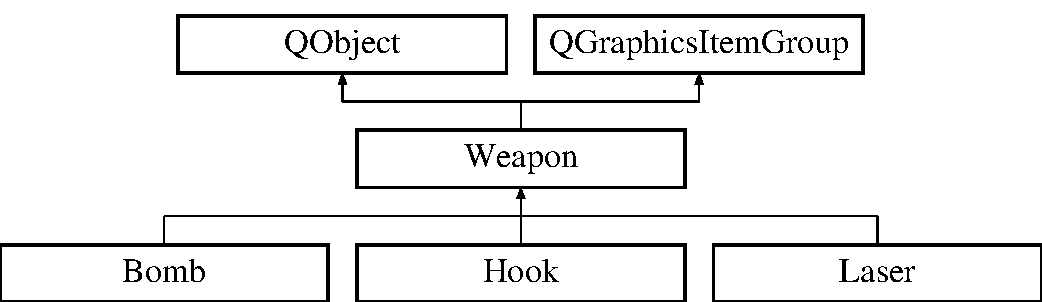
\includegraphics[height=3.000000cm]{classWeapon}
\end{center}
\end{figure}
\subsection*{Public Slots}
\begin{DoxyCompactItemize}
\item 
\hypertarget{classWeapon_a1b3f76c5275b67f0bb8073157a27e736}{virtual void {\bfseries update} ()}\label{classWeapon_a1b3f76c5275b67f0bb8073157a27e736}

\end{DoxyCompactItemize}
\subsection*{Public Member Functions}
\begin{DoxyCompactItemize}
\item 
\hypertarget{classWeapon_a2795df670e0b34ac1fe20bb51ba0cfeb}{{\bfseries Weapon} (Q\-Object $\ast$parent=nullptr)}\label{classWeapon_a2795df670e0b34ac1fe20bb51ba0cfeb}

\end{DoxyCompactItemize}
\subsection*{Public Attributes}
\begin{DoxyCompactItemize}
\item 
\hypertarget{classWeapon_a99ca3e2f3038f934c8eafa5faa0f277e}{Q\-Graphics\-Pixmap\-Item $\ast$ {\bfseries head}}\label{classWeapon_a99ca3e2f3038f934c8eafa5faa0f277e}

\item 
\hypertarget{classWeapon_a9520da53d4a8fc16809e0569e2f1ee19}{Q\-Graphics\-Line\-Item $\ast$ {\bfseries rope}}\label{classWeapon_a9520da53d4a8fc16809e0569e2f1ee19}

\item 
\hypertarget{classWeapon_ace482a60a7ff5d0e6e3ffec0ac9d08ee}{Q\-Graphics\-Item $\ast$ {\bfseries grabbed\-Item}}\label{classWeapon_ace482a60a7ff5d0e6e3ffec0ac9d08ee}

\item 
\hypertarget{classWeapon_ae3fe71083afa9e426faed0d81af6bdb8}{Q\-Timer $\ast$ {\bfseries throw\-Timer}}\label{classWeapon_ae3fe71083afa9e426faed0d81af6bdb8}

\item 
\hypertarget{classWeapon_ad9b695b441f96e232409ebde76cb23ac}{Q\-Timer $\ast$ {\bfseries prepare\-Timer}}\label{classWeapon_ad9b695b441f96e232409ebde76cb23ac}

\item 
\hypertarget{classWeapon_a40c0c9733eb82073858f1b7cc492d386}{Q\-String {\bfseries name}}\label{classWeapon_a40c0c9733eb82073858f1b7cc492d386}

\item 
\hypertarget{classWeapon_a2cbddccb0e512b94787d7c0668529271}{bool {\bfseries thrown}}\label{classWeapon_a2cbddccb0e512b94787d7c0668529271}

\item 
\hypertarget{classWeapon_aac8669fed357d52b5d6d3b32a74feb54}{bool {\bfseries grabbing\-Item}}\label{classWeapon_aac8669fed357d52b5d6d3b32a74feb54}

\item 
\hypertarget{classWeapon_ae62708c1d3be48ce1a4cf2418dec52f3}{bool {\bfseries ready}}\label{classWeapon_ae62708c1d3be48ce1a4cf2418dec52f3}

\item 
\hypertarget{classWeapon_a05703d93b6af2486abd60e2493bbe37e}{int {\bfseries step}}\label{classWeapon_a05703d93b6af2486abd60e2493bbe37e}

\item 
\hypertarget{classWeapon_a4a9381f1b461ca75cf0928defe49fbc0}{int {\bfseries strength}}\label{classWeapon_a4a9381f1b461ca75cf0928defe49fbc0}

\end{DoxyCompactItemize}


The documentation for this class was generated from the following files\-:\begin{DoxyCompactItemize}
\item 
weapon.\-h\item 
\hyperlink{weapon_8cpp}{weapon.\-cpp}\end{DoxyCompactItemize}

\hypertarget{classWelcome}{\section{Welcome Class Reference}
\label{classWelcome}\index{Welcome@{Welcome}}
}
Inheritance diagram for Welcome\-:\begin{figure}[H]
\begin{center}
\leavevmode
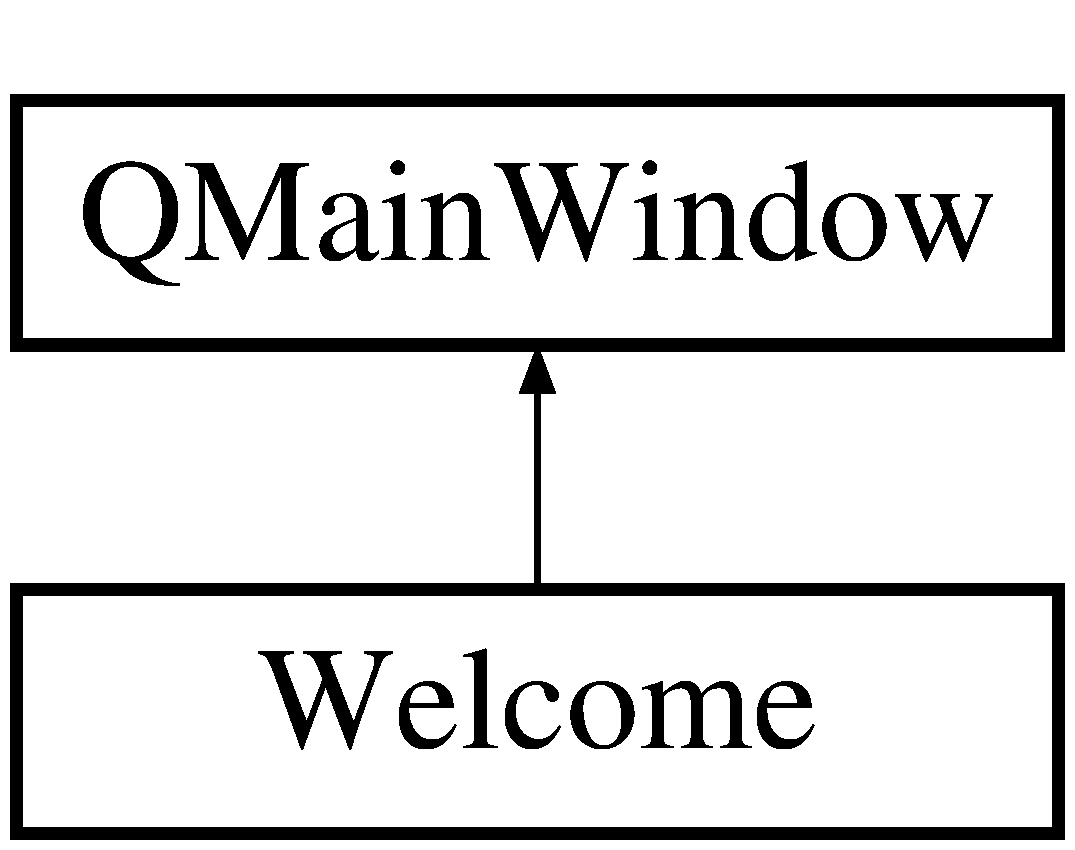
\includegraphics[height=2.000000cm]{classWelcome}
\end{center}
\end{figure}
\subsection*{Public Member Functions}
\begin{DoxyCompactItemize}
\item 
\hypertarget{classWelcome_acf62624f1107ddc68761d25febbf10ad}{{\bfseries Welcome} (Q\-Widget $\ast$parent=0)}\label{classWelcome_acf62624f1107ddc68761d25febbf10ad}

\end{DoxyCompactItemize}


The documentation for this class was generated from the following files\-:\begin{DoxyCompactItemize}
\item 
welcome.\-h\item 
\hyperlink{welcome_8cpp}{welcome.\-cpp}\end{DoxyCompactItemize}

\chapter{File Documentation}
\hypertarget{babyspongebob_8cpp}{\section{babyspongebob.\-cpp File Reference}
\label{babyspongebob_8cpp}\index{babyspongebob.\-cpp@{babyspongebob.\-cpp}}
}


\hyperlink{classBabySpongeBob}{Baby\-Sponge\-Bob} class definition.  


{\ttfamily \#include \char`\"{}babyspongebob.\-h\char`\"{}}\\*
{\ttfamily \#include \char`\"{}grabbable.\-h\char`\"{}}\\*
{\ttfamily \#include $<$Q\-Graphics\-Scene$>$}\\*


\subsection{Detailed Description}
\hyperlink{classBabySpongeBob}{Baby\-Sponge\-Bob} class definition. a \hyperlink{classBabySpongeBob}{Baby\-Sponge\-Bob} is an object in the game that resides on the side of the scene, and should be fed healthy items to win the game \begin{DoxyAuthor}{Author}
Bilal Natafgi 
\end{DoxyAuthor}
\begin{DoxyDate}{Date}
10-\/4-\/2018 
\end{DoxyDate}

\hypertarget{bacteria_8cpp}{\section{bacteria.\-cpp File Reference}
\label{bacteria_8cpp}\index{bacteria.\-cpp@{bacteria.\-cpp}}
}


bacteria class definition  


{\ttfamily \#include \char`\"{}bacteria.\-h\char`\"{}}\\*
{\ttfamily \#include \char`\"{}stdlib.\-h\char`\"{}}\\*
{\ttfamily \#include \char`\"{}game1.\-h\char`\"{}}\\*
{\ttfamily \#include \char`\"{}game2.\-h\char`\"{}}\\*
{\ttfamily \#include \char`\"{}hook.\-h\char`\"{}}\\*


\subsection{Detailed Description}
bacteria class definition a bacteria is an object in the game that gets eaten by the bear when they collide \begin{DoxyAuthor}{Author}
Abdel Jawad Alami 
\end{DoxyAuthor}
\begin{DoxyDate}{Date}
22-\/2-\/2018 
\end{DoxyDate}

\hypertarget{bomb_8cpp}{\section{bomb.\-cpp File Reference}
\label{bomb_8cpp}\index{bomb.\-cpp@{bomb.\-cpp}}
}


\hyperlink{classBomb}{Bomb} class definition.  


{\ttfamily \#include \char`\"{}bomb.\-h\char`\"{}}\\*
{\ttfamily \#include $<$Q\-Pen$>$}\\*
{\ttfamily \#include \char`\"{}sponge\-Bob.\-h\char`\"{}}\\*
{\ttfamily \#include $<$game2scene.\-h$>$}\\*
{\ttfamily \#include \char`\"{}hu\-Item.\-h\char`\"{}}\\*
{\ttfamily \#include $<$Q\-Pointer$>$}\\*
{\ttfamily \#include \char`\"{}grabbable.\-h\char`\"{}}\\*


\subsection{Detailed Description}
\hyperlink{classBomb}{Bomb} class definition. a \hyperlink{classBomb}{Bomb} is an object in the game that can be shot if a specific score is reached. it cleares the area it hits \begin{DoxyAuthor}{Author}
Bilal Natafgi 
\end{DoxyAuthor}
\begin{DoxyDate}{Date}
12-\/4-\/2018 
\end{DoxyDate}

\hypertarget{cheat_8cpp}{\section{cheat.\-cpp File Reference}
\label{cheat_8cpp}\index{cheat.\-cpp@{cheat.\-cpp}}
}


cheat class definition  


{\ttfamily \#include \char`\"{}cheat.\-h\char`\"{}}\\*
{\ttfamily \#include \char`\"{}ui\-\_\-cheat.\-h\char`\"{}}\\*


\subsection{Detailed Description}
cheat class definition T\-O\-D\-O \begin{DoxyAuthor}{Author}
Bilal Natafgi 
\end{DoxyAuthor}
\begin{DoxyDate}{Date}
22-\/3-\/2018 
\end{DoxyDate}

\hypertarget{description_8cpp}{\section{description.\-cpp File Reference}
\label{description_8cpp}\index{description.\-cpp@{description.\-cpp}}
}


\hyperlink{classDescription}{Description} class definition.  


{\ttfamily \#include \char`\"{}description.\-h\char`\"{}}\\*
{\ttfamily \#include \char`\"{}ui\-\_\-description.\-h\char`\"{}}\\*
{\ttfamily \#include \char`\"{}game1.\-h\char`\"{}}\\*


\subsection{Detailed Description}
\hyperlink{classDescription}{Description} class definition. \begin{DoxyAuthor}{Author}
Bilal Natafgi 
\end{DoxyAuthor}
\begin{DoxyDate}{Date}
21-\/3-\/2018 
\end{DoxyDate}

\hypertarget{error_8cpp}{\section{error.\-cpp File Reference}
\label{error_8cpp}\index{error.\-cpp@{error.\-cpp}}
}


\hyperlink{classError}{Error} class definition.  


{\ttfamily \#include \char`\"{}error.\-h\char`\"{}}\\*
{\ttfamily \#include \char`\"{}ui\-\_\-error.\-h\char`\"{}}\\*


\subsection{Detailed Description}
\hyperlink{classError}{Error} class definition. \begin{DoxyAuthor}{Author}
Bilal Natafgi 
\end{DoxyAuthor}
\begin{DoxyDate}{Date}
21-\/3-\/2018 
\end{DoxyDate}

\hypertarget{fungus_8cpp}{\section{fungus.\-cpp File Reference}
\label{fungus_8cpp}\index{fungus.\-cpp@{fungus.\-cpp}}
}


bacteria class definition  


{\ttfamily \#include \char`\"{}fungus.\-h\char`\"{}}\\*
{\ttfamily \#include \char`\"{}stdlib.\-h\char`\"{}}\\*
{\ttfamily \#include \char`\"{}game1.\-h\char`\"{}}\\*
{\ttfamily \#include \char`\"{}game2.\-h\char`\"{}}\\*


\subsection{Detailed Description}
bacteria class definition a fungus is an object in the game that if eaten by the spongebob, spongebob would loose a life, total strength, and aquariom cleanlines would decrease by half \begin{DoxyAuthor}{Author}
Abdel Jawad Alami 
\end{DoxyAuthor}
\begin{DoxyDate}{Date}
25-\/3-\/2018 
\end{DoxyDate}

\hypertarget{game1_8cpp}{\section{game1.\-cpp File Reference}
\label{game1_8cpp}\index{game1.\-cpp@{game1.\-cpp}}
}


game1 class definition  


{\ttfamily \#include \char`\"{}game1.\-h\char`\"{}}\\*
{\ttfamily \#include \char`\"{}ui\-\_\-game1.\-h\char`\"{}}\\*
{\ttfamily \#include $<$Q\-Graphics\-Item$>$}\\*
{\ttfamily \#include $<$Q\-Graphics\-Rect\-Item$>$}\\*
{\ttfamily \#include $<$Q\-Graphics\-Scene$>$}\\*
{\ttfamily \#include $<$Q\-Graphics\-View$>$}\\*
{\ttfamily \#include \char`\"{}game1scene.\-h\char`\"{}}\\*
{\ttfamily \#include \char`\"{}gameview.\-h\char`\"{}}\\*


\subsection{Detailed Description}
game1 class definition the class game1 is used to select the difficulty of the game, add the score and create the scene of game1 \begin{DoxyAuthor}{Author}
Bilal Natafgi 
\end{DoxyAuthor}
\begin{DoxyDate}{Date}
21-\/2-\/2018 
\end{DoxyDate}

\hypertarget{game1scene_8cpp}{\section{game1scene.\-cpp File Reference}
\label{game1scene_8cpp}\index{game1scene.\-cpp@{game1scene.\-cpp}}
}


\hyperlink{classgame1scene}{game1scene} class definition  


{\ttfamily \#include \char`\"{}game1scene.\-h\char`\"{}}\\*
{\ttfamily \#include \char`\"{}stdlib.\-h\char`\"{}}\\*
{\ttfamily \#include $<$Q\-Graphics\-Proxy\-Widget$>$}\\*
{\ttfamily \#include $<$Q\-Graphics\-Ellipse\-Item$>$}\\*
{\ttfamily \#include $<$Q\-Painter$>$}\\*
{\ttfamily \#include $<$Q\-Graphics\-Linear\-Layout$>$}\\*
{\ttfamily \#include $<$Q\-Color\-Dialog$>$}\\*
{\ttfamily \#include \char`\"{}game1.\-h\char`\"{}}\\*
{\ttfamily \#include \char`\"{}scores.\-h\char`\"{}}\\*


\subsection{Detailed Description}
\hyperlink{classgame1scene}{game1scene} class definition a \hyperlink{classgame1scene}{game1scene} contains all the interactions in the game \begin{DoxyAuthor}{Author}
Abdel Jawad Alami 
\end{DoxyAuthor}
\begin{DoxyDate}{Date}
22-\/2-\/2018 
\end{DoxyDate}

\hypertarget{game2_8cpp}{\section{game2.\-cpp File Reference}
\label{game2_8cpp}\index{game2.\-cpp@{game2.\-cpp}}
}


\hyperlink{classGame2}{Game2} class definition.  


{\ttfamily \#include \char`\"{}game2.\-h\char`\"{}}\\*
{\ttfamily \#include \char`\"{}ui\-\_\-game2.\-h\char`\"{}}\\*
{\ttfamily \#include \char`\"{}gameview.\-h\char`\"{}}\\*
{\ttfamily \#include \char`\"{}game2scene.\-h\char`\"{}}\\*


\subsection{Detailed Description}
\hyperlink{classGame2}{Game2} class definition. a \hyperlink{classGame2}{Game2} is where the user selects the strength of the game to play \begin{DoxyAuthor}{Author}
Bilal Natafgi 
\end{DoxyAuthor}
\begin{DoxyDate}{Date}
22-\/2-\/2018 
\end{DoxyDate}

\hypertarget{gamemenu_8cpp}{\section{gamemenu.\-cpp File Reference}
\label{gamemenu_8cpp}\index{gamemenu.\-cpp@{gamemenu.\-cpp}}
}


\hyperlink{classGamemenu}{Gamemenu} class definition.  


{\ttfamily \#include \char`\"{}gamemenu.\-h\char`\"{}}\\*
{\ttfamily \#include \char`\"{}ui\-\_\-gamemenu.\-h\char`\"{}}\\*
{\ttfamily \#include \char`\"{}game1scene.\-h\char`\"{}}\\*
{\ttfamily \#include \char`\"{}game2scene.\-h\char`\"{}}\\*
{\ttfamily \#include \char`\"{}gameview.\-h\char`\"{}}\\*
{\ttfamily \#include \char`\"{}game.\-h\char`\"{}}\\*
{\ttfamily \#include \char`\"{}error.\-h\char`\"{}}\\*


\subsection{Detailed Description}
\hyperlink{classGamemenu}{Gamemenu} class definition. a \hyperlink{classGamemenu}{Gamemenu} is where the user can enter the games, or check his highscore and game descriptiond \begin{DoxyAuthor}{Author}
Bilal Natafgi 
\end{DoxyAuthor}
\begin{DoxyDate}{Date}
20-\/2-\/2018 
\end{DoxyDate}

\hypertarget{gameview_8cpp}{\section{gameview.\-cpp File Reference}
\label{gameview_8cpp}\index{gameview.\-cpp@{gameview.\-cpp}}
}


gameview class definition  


{\ttfamily \#include \char`\"{}gameview.\-h\char`\"{}}\\*
{\ttfamily \#include \char`\"{}ui\-\_\-gameview.\-h\char`\"{}}\\*


\subsection{Detailed Description}
gameview class definition a gameview is where the game scene resides \begin{DoxyAuthor}{Author}
Bilal Natafgi 
\end{DoxyAuthor}
\begin{DoxyDate}{Date}
20-\/2-\/2018 
\end{DoxyDate}

\hypertarget{grabbable_8cpp}{\section{grabbable.\-cpp File Reference}
\label{grabbable_8cpp}\index{grabbable.\-cpp@{grabbable.\-cpp}}
}


\hyperlink{classGrabbable}{Grabbable} class definition.  


{\ttfamily \#include \char`\"{}grabbable.\-h\char`\"{}}\\*
{\ttfamily \#include \char`\"{}hu\-Item.\-h\char`\"{}}\\*
{\ttfamily \#include \char`\"{}bomb.\-h\char`\"{}}\\*
{\ttfamily \#include \char`\"{}laser.\-h\char`\"{}}\\*


\subsection{Detailed Description}
\hyperlink{classGrabbable}{Grabbable} class definition. the grabbable class is excited when an item collides with a weapon or a hook \begin{DoxyAuthor}{Author}
Bilal Natafgi 
\end{DoxyAuthor}
\begin{DoxyDate}{Date}
20-\/2-\/2018 
\end{DoxyDate}

\hypertarget{header_8cpp}{\section{header.\-cpp File Reference}
\label{header_8cpp}\index{header.\-cpp@{header.\-cpp}}
}


\hyperlink{classHeader}{Header} class definition.  


{\ttfamily \#include \char`\"{}header.\-h\char`\"{}}\\*
{\ttfamily \#include \char`\"{}user.\-h\char`\"{}}\\*
{\ttfamily \#include \char`\"{}game1scene.\-h\char`\"{}}\\*
{\ttfamily \#include \char`\"{}game2scene.\-h\char`\"{}}\\*
{\ttfamily \#include $<$Q\-Application$>$}\\*
{\ttfamily \#include \char`\"{}game1.\-h\char`\"{}}\\*
{\ttfamily \#include \char`\"{}game2.\-h\char`\"{}}\\*


\subsection{Detailed Description}
\hyperlink{classHeader}{Header} class definition. the \hyperlink{classHeader}{Header} contains most of the metrics in the game. it contains the difficulty of the game, the username of the player, the timer, the cleanliness of the tank in game one, and henumber of healthy items fed to the baby in game 2. the header contains all items that are located at the top of the game scene. \begin{DoxyAuthor}{Author}
Bilal Natafgi 
\end{DoxyAuthor}
\begin{DoxyDate}{Date}
20-\/2-\/2018 
\end{DoxyDate}

\hypertarget{history_8cpp}{\section{history.\-cpp File Reference}
\label{history_8cpp}\index{history.\-cpp@{history.\-cpp}}
}


history class definition  


{\ttfamily \#include \char`\"{}history.\-h\char`\"{}}\\*
{\ttfamily \#include \char`\"{}ui\-\_\-history.\-h\char`\"{}}\\*


\subsection{Detailed Description}
history class definition the history contains previous scores of a given player.

\begin{DoxyAuthor}{Author}
Bilal Natafgi 
\end{DoxyAuthor}
\begin{DoxyDate}{Date}
23-\/2-\/2018 
\end{DoxyDate}

\hypertarget{home_8cpp}{\section{home.\-cpp File Reference}
\label{home_8cpp}\index{home.\-cpp@{home.\-cpp}}
}


home class definition  


{\ttfamily \#include \char`\"{}home.\-h\char`\"{}}\\*
{\ttfamily \#include \char`\"{}ui\-\_\-home.\-h\char`\"{}}\\*


\subsection{Detailed Description}
home class definition the home page is where the user is redirected after signing in.

\begin{DoxyAuthor}{Author}
Bilal Natafgi 
\end{DoxyAuthor}
\begin{DoxyDate}{Date}
23-\/2-\/2018 
\end{DoxyDate}

\hypertarget{hook_8cpp}{\section{hook.\-cpp File Reference}
\label{hook_8cpp}\index{hook.\-cpp@{hook.\-cpp}}
}


hook class definition  


{\ttfamily \#include \char`\"{}hook.\-h\char`\"{}}\\*
{\ttfamily \#include $<$Q\-Pen$>$}\\*
{\ttfamily \#include \char`\"{}sponge\-Bob.\-h\char`\"{}}\\*
{\ttfamily \#include $<$Q\-Graphics\-Scene$>$}\\*
{\ttfamily \#include \char`\"{}bacteria.\-h\char`\"{}}\\*
{\ttfamily \#include \char`\"{}hu\-Item.\-h\char`\"{}}\\*
{\ttfamily \#include \char`\"{}virus.\-h\char`\"{}}\\*
{\ttfamily \#include \char`\"{}fungus.\-h\char`\"{}}\\*
{\ttfamily \#include $<$Q\-Pointer$>$}\\*
{\ttfamily \#include \char`\"{}grabbable.\-h\char`\"{}}\\*


\subsection{Detailed Description}
hook class definition the hookis a type of weapons by which the player grabs items

\begin{DoxyAuthor}{Author}
Bilal Natafgi 
\end{DoxyAuthor}
\begin{DoxyDate}{Date}
13-\/4-\/2018 
\end{DoxyDate}

\hypertarget{huItem_8cpp}{\section{hu\-Item.\-cpp File Reference}
\label{huItem_8cpp}\index{hu\-Item.\-cpp@{hu\-Item.\-cpp}}
}


\hyperlink{classhuItem}{hu\-Item} class definition  


{\ttfamily \#include \char`\"{}hu\-Item.\-h\char`\"{}}\\*
{\ttfamily \#include \char`\"{}stdlib.\-h\char`\"{}}\\*
{\ttfamily \#include \char`\"{}game1.\-h\char`\"{}}\\*
{\ttfamily \#include \char`\"{}game2.\-h\char`\"{}}\\*


\subsection{Detailed Description}
\hyperlink{classhuItem}{hu\-Item} class definition a \hyperlink{classhuItem}{hu\-Item} is an object in the game that gets eaten by the spongebob when they collide, or by baby spongebob \begin{DoxyAuthor}{Author}
Abdel Jawad Alami 
\end{DoxyAuthor}
\begin{DoxyDate}{Date}
22-\/2-\/2018 
\end{DoxyDate}

\hypertarget{scores_8cpp}{\section{scores.\-cpp File Reference}
\label{scores_8cpp}\index{scores.\-cpp@{scores.\-cpp}}
}


scores class definition  


{\ttfamily \#include \char`\"{}scores.\-h\char`\"{}}\\*


\subsection{Detailed Description}
scores class definition the scores class \begin{DoxyAuthor}{Author}
Bilal natafgi 
\end{DoxyAuthor}
\begin{DoxyDate}{Date}
26-\/2-\/2018 
\end{DoxyDate}

\hypertarget{signin_8cpp}{\section{signin.\-cpp File Reference}
\label{signin_8cpp}\index{signin.\-cpp@{signin.\-cpp}}
}


\hyperlink{classSignIn}{Sign\-In} class definition.  


{\ttfamily \#include \char`\"{}signin.\-h\char`\"{}}\\*
{\ttfamily \#include \char`\"{}ui\-\_\-signin.\-h\char`\"{}}\\*
{\ttfamily \#include \char`\"{}error.\-h\char`\"{}}\\*


\subsection{Detailed Description}
\hyperlink{classSignIn}{Sign\-In} class definition. the \hyperlink{classSignIn}{Sign\-In} class \begin{DoxyAuthor}{Author}
Bilal natafgi 
\end{DoxyAuthor}
\begin{DoxyDate}{Date}
20-\/2-\/2018 
\end{DoxyDate}

\hypertarget{signup_8cpp}{\section{signup.\-cpp File Reference}
\label{signup_8cpp}\index{signup.\-cpp@{signup.\-cpp}}
}


signup class definition  


{\ttfamily \#include \char`\"{}signup.\-h\char`\"{}}\\*
{\ttfamily \#include \char`\"{}ui\-\_\-signup.\-h\char`\"{}}\\*


\subsection{Detailed Description}
signup class definition the signup class \begin{DoxyAuthor}{Author}
Bilal natafgi 
\end{DoxyAuthor}
\begin{DoxyDate}{Date}
20-\/2-\/2018 
\end{DoxyDate}

\hypertarget{spongeBob_8cpp}{\section{sponge\-Bob.\-cpp File Reference}
\label{spongeBob_8cpp}\index{sponge\-Bob.\-cpp@{sponge\-Bob.\-cpp}}
}


sponge\-Bob class definition  


{\ttfamily \#include \char`\"{}sponge\-Bob.\-h\char`\"{}}\\*
{\ttfamily \#include \char`\"{}game1scene.\-h\char`\"{}}\\*
{\ttfamily \#include \char`\"{}game1.\-h\char`\"{}}\\*
{\ttfamily \#include \char`\"{}game2.\-h\char`\"{}}\\*
{\ttfamily \#include \char`\"{}laser.\-h\char`\"{}}\\*
{\ttfamily \#include \char`\"{}hook.\-h\char`\"{}}\\*
{\ttfamily \#include \char`\"{}bomb.\-h\char`\"{}}\\*
{\ttfamily \#include \char`\"{}game2scene.\-h\char`\"{}}\\*
\subsection*{Variables}
\begin{DoxyCompactItemize}
\item 
Q\-Set$<$ int $>$ \hyperlink{spongeBob_8cpp_a35800fcfa62e517c88410e30f5866a93}{pressed\-Keys}
\begin{DoxyCompactList}\small\item\em sponge\-Bob\-::key\-Press\-Event \end{DoxyCompactList}\end{DoxyCompactItemize}


\subsection{Detailed Description}
sponge\-Bob class definition a sponge\-Bob instance \begin{DoxyAuthor}{Author}
Abdel Jawad Alami 
\end{DoxyAuthor}
\begin{DoxyDate}{Date}
18-\/3-\/2018 
\end{DoxyDate}


\subsection{Variable Documentation}
\hypertarget{spongeBob_8cpp_a35800fcfa62e517c88410e30f5866a93}{\index{sponge\-Bob.\-cpp@{sponge\-Bob.\-cpp}!pressed\-Keys@{pressed\-Keys}}
\index{pressed\-Keys@{pressed\-Keys}!spongeBob.cpp@{sponge\-Bob.\-cpp}}
\subsubsection[{pressed\-Keys}]{\setlength{\rightskip}{0pt plus 5cm}Q\-Set$<$int$>$ pressed\-Keys}}\label{spongeBob_8cpp_a35800fcfa62e517c88410e30f5866a93}


sponge\-Bob\-::key\-Press\-Event 


\begin{DoxyParams}{Parameters}
{\em event} & the keypress event detects all key strokes on the keyboard. we are only interested in the up,down,left, and right strokes when one of those keys is pressed, the bear moves accoringly when possible if the location of the bear is on the edges of the screen, the position isnt updated if this will result in leaving the screen \\
\hline
\end{DoxyParams}

\hypertarget{virus_8cpp}{\section{virus.\-cpp File Reference}
\label{virus_8cpp}\index{virus.\-cpp@{virus.\-cpp}}
}


virus class definition  


{\ttfamily \#include \char`\"{}virus.\-h\char`\"{}}\\*
{\ttfamily \#include \char`\"{}stdlib.\-h\char`\"{}}\\*
{\ttfamily \#include \char`\"{}game1.\-h\char`\"{}}\\*
{\ttfamily \#include \char`\"{}game2.\-h\char`\"{}}\\*


\subsection{Detailed Description}
virus class definition a virus is an object in the game that if eaten by spongebob, makes the bacteria follow him. \begin{DoxyAuthor}{Author}
Abdel Jawad Alami 
\end{DoxyAuthor}
\begin{DoxyDate}{Date}
18-\/3-\/2018 
\end{DoxyDate}

\hypertarget{weapon_8cpp}{\section{weapon.\-cpp File Reference}
\label{weapon_8cpp}\index{weapon.\-cpp@{weapon.\-cpp}}
}


weapon class definition  


{\ttfamily \#include \char`\"{}weapon.\-h\char`\"{}}\\*


\subsection{Detailed Description}
weapon class definition this weapon class is an abstract class that all weapons inherit from. \begin{DoxyAuthor}{Author}
Abdel Jawad Alami 
\end{DoxyAuthor}
\begin{DoxyDate}{Date}
18-\/3-\/2018 
\end{DoxyDate}

\hypertarget{welcome_8cpp}{\section{welcome.\-cpp File Reference}
\label{welcome_8cpp}\index{welcome.\-cpp@{welcome.\-cpp}}
}


welcome class definition  


{\ttfamily \#include \char`\"{}welcome.\-h\char`\"{}}\\*
{\ttfamily \#include \char`\"{}ui\-\_\-welcome.\-h\char`\"{}}\\*
{\ttfamily \#include \char`\"{}signup.\-h\char`\"{}}\\*
{\ttfamily \#include \char`\"{}signin.\-h\char`\"{}}\\*


\subsection{Detailed Description}
welcome class definition welcome class with its functions \begin{DoxyAuthor}{Author}
Bilal Natafgi 
\end{DoxyAuthor}
\begin{DoxyDate}{Date}
18-\/3-\/2018 
\end{DoxyDate}

%--- End generated contents ---

% Index
\newpage
\phantomsection
\addcontentsline{toc}{chapter}{Index}
\printindex

\end{document}
